\documentclass[
		twoside,
		openright,
		titlepage,
		numbers=noenddot
		,headinclude,%1headlines,
	 	footinclude=true,
	 	cleardoublepage=empty,
		dottedtoc, % Make page numbers in the table of contents flushed right with dots leading to them
		BCOR=5mm,paper=a4,fontsize=11pt, % Binding correction, paper type and font size
		american % Languages, change this to your language(s)
		]{scrreprt}

% Includes the file which contains all the document configurations and packages - make sure to edit this file
%%%%%%%%%%%%%%%%%%%%%%%%%%%%%%%%%%%%%%%%%
% Classicthesis Typographic Thesis
% Configuration File
%
% This file has been downloaded from:
% http://www.LaTeXTemplates.com
%
% Original author:
% André Miede (http://www.miede.de) with extensive commenting changes by:
% Vel (vel@LaTeXTemplates.com)
%
% License:
% GNU General Public License (v2)
%
% Important note:
% The main lines to change in this file are in the DOCUMENT VARIABLES
% section, the rest of the file is for advanced configuration.
%
%%%%%%%%%%%%%%%%%%%%%%%%%%%%%%%%%%%%%%%%%

%----------------------------------------------------------------------------------------
%	CHARACTER ENCODING
%----------------------------------------------------------------------------------------

\PassOptionsToPackage{utf8}{inputenc} % Set the encoding of your files. UTF-8 is the only sensible encoding nowadays. If you can't read äöüßáéçèê∂åëæƒÏ€ then change the encoding setting in your editor, not the line below. If your editor does not support utf8 use another editor!
\usepackage{inputenc}

%----------------------------------------------------------------------------------------
%	DOCUMENT VARIABLES
%	Fill in the lines below to enter your information into the thesis template
%	Each of the commands can be cited anywhere in the thesis
%----------------------------------------------------------------------------------------

% Remove drafting to get rid of the '[ Date - classicthesis version 4.0 ]' text at the bottom of every page
\PassOptionsToPackage{eulerchapternumbers,drafting, pdfspacing, subfig,beramono,eulermath,parts}{classicthesis}
% Available options: drafting parts nochapters linedheaders eulerchapternumbers beramono eulermath pdfspacing minionprospacing tocaligned dottedtoc manychapters listings floatperchapter subfig

\newcommand{\myTitle}{Deep Learning Next Event Prediction With Subsequence-Enrichted Input Data}
\newcommand{\mySubtitle}{An Homage to The Elements of Typographic Style\xspace}
\newcommand{\myDegree}{Master Of Science\xspace}
\newcommand{\myName}{Felix Wolff\xspace}
\newcommand{\myProf}{Prof. Dr. Mathias Weske\xspace}
\newcommand{\myOtherProf}{???????\xspace}
\newcommand{\mySupervisorA}{Dr. Luise Pufahl}
\newcommand{\mySupervisorB}{Dr. Haojin Yang}
\newcommand{\myFaculty}{Business Process Technology Group}
\newcommand{\myDepartment}{Put data here\xspace}
\newcommand{\myUni}{Hasso Plattner Institut}
\newcommand{\myLocation}{Potsdam\xspace}
\newcommand{\myTime}{February 20, 2019\xspace}
\newcommand{\myVersion}{version 0.1\xspace}

%----------------------------------------------------------------------------------------
%	USEFUL COMMANDS
%----------------------------------------------------------------------------------------

\newcommand{\ie}{i.\,e.}
\newcommand{\Ie}{I.\,e.}
\newcommand{\eg}{e.\,g.}
\newcommand{\Eg}{E.\,g.} 

\newcounter{dummy} % Necessary for correct hyperlinks (to index, bib, etc.)
\providecommand{\mLyX}{L\kern-.1667em\lower.25em\hbox{Y}\kern-.125emX\@}
\newlength{\abcd} % for ab..z string length calculation

%----------------------------------------------------------------------------------------
%	PACKAGES
%----------------------------------------------------------------------------------------

\usepackage{lipsum} % Used for inserting dummy 'Lorem ipsum' text into the template
\usepackage{todonotes}
\usepackage{amsmath}
\usepackage[utf8]{inputenc}
\usepackage{multicol}
\usepackage{makecell}
\usepackage{subfig}

%------------------------------------------------

%\PassOptionsToPackage{ngerman,american}{babel}  % Change this to your language(s)
% Spanish languages need extra options in order to work with this template
%\PassOptionsToPackage{spanish,es-lcroman}{babel}
\usepackage{babel}

%------------------------------------------------			

\usepackage{csquotes}
\PassOptionsToPackage{%
%backend=biber, % Instead of bibtex
backend=bibtex8,bibencoding=ascii,%
language=auto,%
style=numeric-comp,%
%style=authoryear-comp, % Author 1999, 2010
%bibstyle=authoryear,dashed=false, % dashed: substitute rep. author with ---
sorting=nyt, % name, year, title
maxbibnames=10, % default: 3, et al.
%backref=true,%
natbib=true % natbib compatibility mode (\citep and \citet still work)
}{biblatex}
\usepackage{biblatex}
 
 %------------------------------------------------

\PassOptionsToPackage{fleqn}{amsmath} % Math environments and more by the AMS 
 \usepackage{amsmath}
 
 %------------------------------------------------

\PassOptionsToPackage{T1}{fontenc} % T2A for cyrillics
\usepackage{fontenc}

%------------------------------------------------

\usepackage{textcomp} % Fix warning with missing font shapes

%------------------------------------------------

%\usepackage{scrhack} % Fix warnings when using KOMA with listings package  

%------------------------------------------------

\usepackage{xspace} % To get the spacing after macros right

%------------------------------------------------

\usepackage{mparhack} % To get marginpar right

%------------------------------------------------

\usepackage{fixltx2e} % Fixes some LaTeX stuff 

%------------------------------------------------

\PassOptionsToPackage{smaller}{acronym} % Include printonlyused in the first bracket to only show acronyms used in the text
\usepackage{acronym} % Nice macros for handling all acronyms in the thesis

%\renewcommand*{\acsfont}[1]{\textssc{#1}} % For MinionPro
\renewcommand*{\aclabelfont}[1]{\acsfont{#1}}

%------------------------------------------------

\PassOptionsToPackage{pdftex}{graphicx}
\usepackage{graphicx} 

%----------------------------------------------------------------------------------------
%	FLOATS: TABLES, FIGURES AND CAPTIONS SETUP
%----------------------------------------------------------------------------------------

\usepackage{tabularx} % Better tables
\setlength{\extrarowheight}{3pt} % Increase table row height
\newcommand{\tableheadline}[1]{\multicolumn{1}{c}{\spacedlowsmallcaps{#1}}}
\newcommand{\myfloatalign}{\centering} % To be used with each float for alignment
\usepackage{caption}
\captionsetup{font=small}

%----------------------------------------------------------------------------------------
%	CODE LISTINGS SETUP
%----------------------------------------------------------------------------------------
\usepackage{minted}
\usemintedstyle{friendly}
\setminted{
    autogobble=true,
    breaklines=true
    linenos=true}
\providecommand*{\listingautorefname}{Listing}

%----------------------------------------------------------------------------------------
%	HYPERREFERENCES
%----------------------------------------------------------------------------------------

\PassOptionsToPackage{pdftex,hyperfootnotes=false,pdfpagelabels}{hyperref}
\usepackage{hyperref}  % backref linktocpage pagebackref
\pdfcompresslevel=9
\pdfadjustspacing=1

\hypersetup{
% Uncomment the line below to remove all links (to references, figures, tables, etc), useful for b/w printouts
%draft, 
colorlinks=true, linktocpage=true, pdfstartpage=3, pdfstartview=FitV,
% Uncomment the line below if you want to have black links (e.g. for printing black and white)
%colorlinks=false, linktocpage=false, pdfborder={0 0 0}, pdfstartpage=3, pdfstartview=FitV, 
breaklinks=true, pdfpagemode=UseNone, pageanchor=true, pdfpagemode=UseOutlines,%
plainpages=false, bookmarksnumbered, bookmarksopen=true, bookmarksopenlevel=1,%
hypertexnames=true, pdfhighlight=/O,%nesting=true,%frenchlinks,%
urlcolor=webbrown, linkcolor=RoyalBlue, citecolor=webgreen, %pagecolor=RoyalBlue,%
    %urlcolor=Black, linkcolor=Black, citecolor=Black, %pagecolor=Black,%
%------------------------------------------------
% PDF file meta-information
pdftitle={\myTitle},
pdfauthor={\textcopyright\ \myName, \myUni, \myFaculty},
pdfsubject={},
pdfkeywords={},
pdfcreator={pdfLaTeX},
pdfproducer={LaTeX with hyperref and classicthesis}
%------------------------------------------------
}

%----------------------------------------------------------------------------------------
%	AUTOREFERENCES SETUP
%	Redefines how references in text are prefaced for different 
%	languages (e.g. "Section 1.2" or "section 1.2")
%----------------------------------------------------------------------------------------

\makeatletter
\@ifpackageloaded{babel}
{
\addto\extrasamerican{
\renewcommand*{\figureautorefname}{Figure}
\renewcommand*{\tableautorefname}{Table}
\renewcommand*{\partautorefname}{Part}
\renewcommand*{\chapterautorefname}{Chapter}
\renewcommand*{\sectionautorefname}{Section}
\renewcommand*{\subsectionautorefname}{Section}
\renewcommand*{\subsubsectionautorefname}{Section}
}
\addto\extrasngerman{
\renewcommand*{\paragraphautorefname}{Absatz}
\renewcommand*{\subparagraphautorefname}{Unterabsatz}
\renewcommand*{\footnoteautorefname}{Fu\"snote}
\renewcommand*{\FancyVerbLineautorefname}{Zeile}
\renewcommand*{\theoremautorefname}{Theorem}
\renewcommand*{\appendixautorefname}{Anhang}
\renewcommand*{\equationautorefname}{Gleichung}
\renewcommand*{\itemautorefname}{Punkt}
}
\providecommand{\subfigureautorefname}{\figureautorefname} % Fix to getting autorefs for subfigures right
}{\relax}
\makeatother

%----------------------------------------------------------------------------------------

\usepackage{classicthesis} 

%----------------------------------------------------------------------------------------
%	CHANGING TEXT AREA 
%----------------------------------------------------------------------------------------

%\linespread{1.05} % a bit more for Palatino
%\areaset[current]{312pt}{761pt} % 686 (factor 2.2) + 33 head + 42 head \the\footskip
%\setlength{\marginparwidth}{7em}%
%\setlength{\marginparsep}{2em}%

%----------------------------------------------------------------------------------------
%	USING DIFFERENT FONTS
%----------------------------------------------------------------------------------------

%\usepackage[oldstylenums]{kpfonts} % oldstyle notextcomp
%\usepackage[osf]{libertine}
%\usepackage[light,condensed,math]{iwona}
%\renewcommand{\sfdefault}{iwona}
%\usepackage{lmodern} % <-- no osf support :-(
%\usepackage{cfr-lm} % 
%\usepackage[urw-garamond]{mathdesign} <-- no osf support :-(
%\usepackage[default,osfigures]{opensans} % scale=0.95 
%\usepackage[sfdefault]{FiraSans}

\addbibresource{Bibliography.bib} % The file housing your bibliography
%\addbibresource[label=ownpubs]{Self_Publications.bib} % Uncomment for optional self-publications

%\hyphenation{SP-2}

\begin{document}

\frenchspacing % Reduces space after periods to make text more compact

\raggedbottom % Makes all pages the height of the text on that page

\selectlanguage{american} % Select your default language - e.g. american or ngerman

%\renewcommand*{\bibname}{new name} % Uncomment to change the name of the bibliography
%\setbibpreamble{} % Uncomment to include a preamble to the bibliography - some text before the reference list starts

\pagenumbering{roman} % Roman page numbering prior to the start of the thesis content (i, ii, iii, etc)

\pagestyle{plain} % Suppress headers for the pre-content pages

%----------------------------------------------------------------------------------------
%	PRE-CONTENT THESIS PAGES
%----------------------------------------------------------------------------------------

% Title Page
\newenvironment{myepigraph}
  {\par\hfill
   \begin{tabular}{@{}r@{\hspace{13em}}}}
  {\end{tabular}\par\medskip}

\begin{titlepage}

\begin{addmargin}[-1cm]{-3cm}
\begin{center}
\large

\hfill
\vfill


\begingroup
  \color{Maroon}\spacedallcaps{\myTitle}:\\
  \color{Maroon}\spacedallcaps{\mySubtitle}\\[1em]
  \color{Black}\spacedlowsmallcaps{\myGermanTitle}\\[3em]
\endgroup

{
\color{Black}
\spacedlowsmallcaps{Master's thesis} | \spacedlowsmallcaps{\myName}\\
\spacedlowsmallcaps{\myTime}
}

\vfill


\includegraphics[width=6cm]{gfx/hpi_logo.jpg} \\[2ex]
\begin{myepigraph}
    \spacedlowsmallcaps{Supervised by}\\[1.1em]
    \myProf\\
    \mySupervisorA\\
    \mySupervisorB\\[1.5em]
    \spacedlowsmallcaps{\myFaculty}
\end{myepigraph}

\myTime\ -- \myVersion % Time and version

\vfill

\end{center}
\end{addmargin}

\end{titlepage}
 % Main title page

% Back of the title page

\thispagestyle{empty}

\hfill

\vfill

\noindent\myName: \textit{\myTitle,} \mySubtitle, %\myDegree, 
\textcopyright\ \myTime

% You may wish to do something with the back of the title page, such as including your supervisors, location or time frame of the work. Below is an example of doing so although you may want to tweak it to your liking.

%\bigskip

%\noindent\spacedlowsmallcaps{Supervisors}: \\
%\myProf \\
%\myOtherProf \\ 
%\mySupervisor

%\medskip \\

%\noindent\spacedlowsmallcaps{Location}: \\
%\myLocation

%\medskip \\

%\noindent\spacedlowsmallcaps{Time Frame}: \\
%\myTime
 % Back of the title page

\cleardoublepage% Dedication

\thispagestyle{empty}
\refstepcounter{dummy}

\pdfbookmark[1]{Dedication}{Dedication} % Bookmark name visible in a PDF viewer

\vspace*{3cm}

\begin{center}
Alles ist relativ \\ \medskip
--- Albert Einstein
\end{center}
 % Dedication page

%\cleardoublepage\include{FrontBackMatter/Foreword} % Uncomment and create a Foreword.tex to include a foreword

\cleardoublepage% Abstract

%\renewcommand{\abstractname}{Abstract} % Uncomment to change the name of the abstract

\pdfbookmark[1]{Abstract}{Abstract} % Bookmark name visible in a PDF viewer

\begingroup
\let\clearpage\relax
\let\cleardoublepage\relax
\let\cleardoublepage\relax

\chapter*{Abstract}
While manual labor processes have seen a lot of automation in the past,
knowledge-intensive processes are still highly manual.
Assistance systems for knowledge work have been asked for in recent several literature reviews.
Such systems need to anticipate the development of a case in order to offer assitance in the right circumstances.
This capability includes the ability to foresee the next activity in a process.

We connect process prediction to sequence prediction, and adapt a successfully tested word prediction model to predict the next activity in a running process.
We implement two published models as baselines to avoid comparability issues due to data preprocessing.
To make model training easier and increase comparability, we also propose a model training framework.

We evaluate our approaches on seven datasets, and compare them to two recent next-activity prediction approaches on a log from BPIC 2012. On this log, we are able to obtain an accuracy of $0.853$, outperforming the compared approaches by approximately $0.05$.

\vfill

\pdfbookmark[1]{German Abstract}{German Abstract}
\chapter*{German Abstract}

\endgroup

\vfill
 % Abstract page

%\cleardoublepage% Publications - a page listing research articles written using content in the thesis

\pdfbookmark[1]{Publications}{Publications} % Bookmark name visible in a PDF viewer

\chapter*{Publications} % Publications page text

Some ideas and figures have appeared previously in the following publications:\\

\noindent Put your publications from the thesis here. The packages \texttt{multibib} or \texttt{bibtopic} etc. can be used to handle multiple different bibliographies in your document.

%\begin{refsection}[ownpubs]
%    \small
%    \nocite{*} % is local to to the enclosing refsection
%    \printbibliography[heading=none]
%\end{refsection}

%\emph{Attention}: This requires a separate run of \texttt{bibtex} for your \texttt{refsection}, \eg, \texttt{ClassicThesis1-blx} for this file. You might also use \texttt{biber} as the backend for \texttt{biblatex}. See also \url{http://tex.stackexchange.com/questions/128196/problem-with-refsection}. % Publications from the thesis page

\cleardoublepage\pdfbookmark[1]{Acknowledgements}{Acknowledgements} % Bookmark name visible in a PDF viewer

\begin{flushright}{\slshape
We have seen that computer programming is an art, \\
because it applies accumulated knowledge to the world, \\
because it requires skill and ingenuity, and especially \\
because it produces objects of beauty.} \\ \medskip
\end{flushright}

\bigskip


\begingroup

\let\clearpage\relax
\let\cleardoublepage\relax
\let\cleardoublepage\relax

\chapter*{Acknowledgements}

Luise Pufahl
Haojin Yang
Feng Cheng

All the sticks out there:
Willi Gierke (LSTM questions)
Marvin Bornstein
Stephan Detje
Georg Berecz
Python Guy für Hilfe when chainer was considered
Stefan Schönig, Richard Jasinski for providing code and help for Schönig\cite{schoenig2018} model
Jörg Evermann for helping with reconstruction of his model\cite{evermann2016}

Special thanks to Jerry B Anderson

My family for food, money, good words\\

Hasso Plattner for building this grand institute and it having so much of an impact on me and my life

\noindent Many thanks to everybody who already sent me a postcard!\\

\noindent Regarding the typography and other help, many thanks go to Marco Kuhlmann, Philipp Lehman, Lothar Schlesier, Jim Young, Lorenzo Pantieri and Enrico Gregorio\footnote{Members of GuIT (Gruppo Italiano Utilizzatori di \TeX\ e \LaTeX )}, J\"org Sommer, Joachim K\"ostler, Daniel Gottschlag, Denis Aydin, Paride Legovini, Steffen Prochnow, Nicolas Repp, Hinrich Harms, Roland Winkler, and the whole \LaTeX-community for support, ideas and some great software.

\bigskip

\noindent\emph{Regarding \mLyX}: The \mLyX\ port was initially done by
\emph{Nicholas Mariette} in March 2009 and continued by
\emph{Ivo Pletikosi\'c} in 2011. Thank you very much for your work and the contributions to the original style.

\endgroup
 % Acknowledgements page

\pagestyle{scrheadings} % Show chapter titles as headings

\cleardoublepage% Table of Contents - List of Tables/Figures/Listings and Acronyms

\refstepcounter{dummy}

\pdfbookmark[1]{\contentsname}{tableofcontents} % Bookmark name visible in a PDF viewer

\setcounter{tocdepth}{1} % Depth of sections to include in the table of contents - currently up to subsections

\setcounter{secnumdepth}{3} % Depth of sections to number in the text itself - currently up to subsubsections

\manualmark
\markboth{\spacedlowsmallcaps{\contentsname}}{\spacedlowsmallcaps{\contentsname}}
\tableofcontents 
\automark[section]{chapter}
\renewcommand{\chaptermark}[1]{\markboth{\spacedlowsmallcaps{#1}}{\spacedlowsmallcaps{#1}}}
\renewcommand{\sectionmark}[1]{\markright{\thesection\enspace\spacedlowsmallcaps{#1}}}

\clearpage

\begingroup 
\let\clearpage\relax
\let\cleardoublepage\relax
\let\cleardoublepage\relax

%----------------------------------------------------------------------------------------
%	List of Figures
%----------------------------------------------------------------------------------------

\refstepcounter{dummy}
%\addcontentsline{toc}{chapter}{\listfigurename} % Uncomment if you would like the list of figures to appear in the table of contents
\pdfbookmark[1]{\listfigurename}{lof} % Bookmark name visible in a PDF viewer

\listoffigures

\vspace{8ex}
\newpage

%----------------------------------------------------------------------------------------
%	List of Tables
%----------------------------------------------------------------------------------------

\refstepcounter{dummy}
%\addcontentsline{toc}{chapter}{\listtablename} % Uncomment if you would like the list of tables to appear in the table of contents
\pdfbookmark[1]{\listtablename}{lot} % Bookmark name visible in a PDF viewer

\listoftables
        
\vspace{8ex}
\newpage
    
%----------------------------------------------------------------------------------------
%	List of Listings
%---------------------------------------------------------------------------------------- 

\refstepcounter{dummy}
%\addcontentsline{toc}{chapter}{\lstlistlistingname} % Uncomment if you would like the list of listings to appear in the table of contents
\pdfbookmark[1]{\lstlistlistingname}{lol} % Bookmark name visible in a PDF viewer

\lstlistoflistings 

\vspace{8ex}
\newpage
       
%----------------------------------------------------------------------------------------
%	Acronyms
%----------------------------------------------------------------------------------------

\refstepcounter{dummy}
%\addcontentsline{toc}{chapter}{Acronyms} % Uncomment if you would like the acronyms to appear in the table of contents
\pdfbookmark[1]{Acronyms}{acronyms} % Bookmark name visible in a PDF viewer

\markboth{\spacedlowsmallcaps{Acronyms}}{\spacedlowsmallcaps{Acronyms}}

\chapter*{Acronyms}

\begin{acronym}[UML]
\acro{DRY}{Don't Repeat Yourself}
\acro{API}{Application Programming Interface}
\acro{NLP}{Natural Language Processing}
\acro{ANN}{Artificial Neural Network}
\acro{SVR}{Support Vector Regression}
\acro{SVM}{Support Vector Machine}
\acro{DFA}{Deterministic Finite Automaton}
\acro{LSTM}{Long Short-Term Memory}
\end{acronym}  
                   
\endgroup % Contents, list of figures/tables/listings and acronyms

\cleardoublepage

\pagenumbering{arabic} % Arabic page numbering for thesis content (1, 2, 3, etc)
%\setcounter{page}{90} % Uncomment to manually start the page counter at an arbitrary value (for example if you wish to count the pre-content pages in the page count)

\cleardoublepage % Avoids problems with pdfbookmark

%----------------------------------------------------------------------------------------
%	THESIS CONTENT - CHAPTERS
%----------------------------------------------------------------------------------------

%\ctparttext{You can put some informational part preamble text here. Illo principalmente su nos. Non message \emph{occidental} angloromanic da. Debitas effortio simplificate sia se, auxiliar summarios da que, se avantiate publicationes via. Pan in terra summarios, capital interlingua se que. Al via multo esser specimen, campo responder que da. Le usate medical addresses pro, europa origine sanctificate nos se.} % Text on the Part 1 page describing  the content in Part 1

%\part{Some Kind of Manual} % First part of the thesis

%\include{Chapters/Chapter01} % Chapter 1

%\cleardoublepage % Empty page before the start of the next part

%------------------------------------------------

%\ctparttext{You can put some informational part preamble text here. Illo principalmente su nos. Non message \emph{occidental} angloromanic da. Debitas effortio simplificate sia se, auxiliar summarios da que, se avantiate publicationes via. Pan in terra summarios, capital interlingua se que. Al via multo esser specimen, campo responder que da. Le usate medical addresses pro, europa origine sanctificate nos se.} % Text on the Part 2 page describing the content in Part 2

%\part{The Showcase} % Second part of the thesis

\chapter{Introduction}\label{sec:intro}
\begin{flushright}{\slshape
I choose a lazy person to do a hard job,\\
because a lazy person will find an easy way to do it.}\\
\medskip
--- Bill Gates
\end{flushright}

\noindent Since the dawn of time, humanity has always tried to find ways to make work easier. With the start of the industrial revolution this was achieved by constructing machines and other helpful contraptions which automated a task. In more recent years, a guiding procedure - a process - was installed to streamline the workflow where a complete automation was not possible. With the rise of the credo "what gets measured, gets managed", key performance indicators (KPIs) were installed into manual labor processes~\cite{web:taylorism-and-drucker} to optimize process efficiency further.\\

However, processes and KPIs fell short of penetrating and improving the realm of knowledge work, since the foundational mechanics of it differ strongly from manual labor. Peter F. Drucker, a renowned management educator, realized this in 1999:
{\slshape"The most important contribution of management in the 20th century was to increase manual worker productivity fifty-fold. The most important contribution of management in the 21st century will be to increase knowledge worker productivity — hopefully by the same percentage"}~\cite{drucker1999}.\\

In the spirit of Drucker's statement and by leveraging the technical developments of the years since his statement, we apply deep learning on business process data to predict the next activity in a running business process by using its execution history. We focus on deep learning methods because they have been shown to outperform others~\cite{tax2018interdisciplinary}. How this is a first step toward process automation in knowledge work, will be explained further in \autoref{sec:intro:motivation}.  We highlight the resulting contribution to current research in \autoref{sec:intro:contribution}. The chapter ends in \autoref{sec:intro:outline} with a description of the thesis outline.

\section{Motivation} \label{sec:intro:motivation}
Automation of work is a phenomenon that has occurred in the past with manual labor, and is spreading into other types of work today, namely knowledge work. As mentioned before, manual labor and knowledge work differ:

The course of manual labour is determined by physical laws, is often very structured, and thus offers great potential for simple automation - like work at an assembly line. Knowledge work on the other hand requires workers to "think for a living", and is strongly shaped by the individuality of the thoughts and habits of each knowledge worker~\cite{drucker1999}. As each worker has a different knowledge background, and uses information differently, this type of work is very flexible and often no process is executed exactly the same~\cite{hewelt2016}. A popular example for knowledge work are insurance claims, handled by several employees. Each claim requires a different course of action, since the information contained in each case differs.\\

In the 20 years since Drucker's mission statement, the analog tools of knowledge workers have evolved into a plethora of digital systems and applications. These help make their decisions more informed and faster. Furthermore, these systems also track work progress, resulting in a large amount of logs which document the course that work on a case, i.e. a running process, has taken.\\

These logs are a valuable source of information as they can reveal best practices that knowledge workers use in certain situations. If this data were processed, such best practices could be recommended by an auxiliary system. These knowledge worker assistance systems have been called for in recent literature reviews by Hauder et al.~\cite{hauder2014} and Francescomarino et al.~\cite{francescomarino2018}, but have only been implemented prototypically until now. One of the challenges that lie in the way of creating assistance systems is the task of anticipating the development of a case, and foreseeing which part comes next. Once then a machine understands the \textit{what} and is only missing the \textit{how}, the ability to forecast process developments can be understood as a step toward process automation.\\

Forecasting the course of a running process can be useful for workers doing either manual labor or knowledge work. Manual labor is often dominated by questions of time and outcome~\cite{rogge2013} because the course of work is clear - natural interests in a world of distributed supply chains and just-in-time production~\cite{web:economist:jit}. The course of the work itself is of interest in the case of unstructured knowledge work~\cite{francescomarino2015}, which is  often unclear, and depends on the information handled inside a case. Knowing about the development of a case presents workers with an opportunity to intervene if it were to progress in an unwanted fashion.\\

By regarding the execution history of an ongoing case, the prediction of its next activity is possible - illustrated in \autoref{fig:next-activity-prediction}. This prediction could then be processed further by the aforementioned assistance system, e.g. to propose an intervention if a case takes an unwanted course. The application of Predictive Analytics on business processes enables this type of prediction. It is fairly new, and is commonly referred to as Predictive Process Monitoring.

\begin{figure}
    \centering
    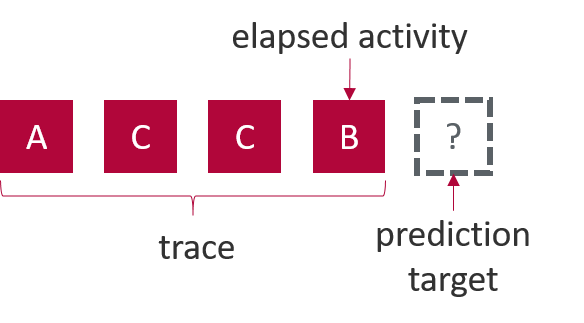
\includegraphics[width=0.7\textwidth]{gfx/next-activity.png}
    \caption[Next-activity prediction from a trace]{The next activity of a case is predicted from the sequence of elapsed activities in its trace}
    \label{fig:next-activity-prediction}
\end{figure}

While working with the literature, we realized that the current research in this young domain can be improved in three areas. These will henceforth be referred to as improvement areas:

\begin{enumerate}
    \item[\textbf{Area 1}] Comparability: Published approaches often use different datasets, making them hard to compare.
    \item[\textbf{Area 2}] Reproducibility: Divergent approaches to training the prediction models and low technical depth of the publications make it hard to reproduce the published results. Furthermore, some prediction approaches are not focused on a single case but whole event streams without specific regard to a case~\cite{evermann2016, schoenig2018}.
    \item[\textbf{Area 3}] NLP-Influence: The history of a case is essentially a sequence, but little inspiration has been taken from Natural Language Processing (NLP), where sequence prediction is common~\cite{shibata2016bipartite}.
\end{enumerate}

\section{Contribution}\label{sec:intro:contribution}
In this work, we make a contribution to ongoing research by applying neural networks on process execution logs to predict the next activity. The work was guided by the three improvement areas.

We address Area 3 by reusing a successful sequence prediction approach from the NLP domain and applying it on business process log data. We also adapt it to incorporate learnings from a paper~\cite{klinkmuller2018reliablemonitoring}. We compare two models to reimplemented prediction models of two published approaches. This provides us with the direct comparability mentioned in Area 1. The models were reverse-engineered from the following publications:

\begin{enumerate}
    \item\textit{A Deep Learning Approach for Predicting Process Behaviour at Runtime} by Evermann et al.~\cite{evermann2016}
    \item\textit{Deep Learning Process Prediction with Discrete and Continuous Data Features} by Schönig et al.~\cite{schoenig2018}.
\end{enumerate}

Over the course of reverse-engineering the comparison models and the subsequent evaluation, widely divergent understandings and approaches with regard to the batch structure of sequential training data input for neural networks were uncovered. To contribute to a better understanding in this area, a comparison of four different batching strategies was incorporated into the evaluation.

As we remarked the comparability of current publications in Area 1, we include a sequence prediction model training framework in this thesis. It allowed us to train four different models with four different batching strategies on seven prepared datasets with ease. It is extensible for other researchers to facilitate comparability among future works.

We use the datasets from the Business Process Intelligence Competition (BPIC) years 2011, 2012, and 2015, where the latter consists of five datasets. The processes in each dataset differ strongly from each other, and we infer a suggestion on which batching strategy could be advantageous to use on which flavor of process log. The use of the BPIC12 dataset furthermore allows for a direct comparison to published next-activity prediction approaches.

We evaluate the trained models using three criteria: First, total accuracy. Second, we test for accuracy stability across the whole execution of the process, which we believe is key for putting trust into the model~\cite{francescomarino2015, boehmer2018probability}. Third, we investigate training time requirements.

From the three evaluation criteria, we reason about the effectiveness of certain model-batching-strategy combinations and finally compare them to published performance figures.

\section{Thesis Outline}\label{sec:intro:outline}
The thesis outline is described in this section. \autoref{chap:background} delivers the necessary background on Process Science and Predictive Analytics. Furthermore it provides information on Predictive Model Development as well as details on the inner workings of the used type of neural network.

\autoref{chap:related-work} gives an overview of current approaches to the prediction task at hand, highlighting the achievements and technicalities of each publication. Furthermore it presents work that was done on the problem of sequence prediction in the field of Natural Language Processing (NLP). For each publication used as comparison, the work is presented with implementation details.

In \autoref{chap:taking-inspiration}, we show how sequences relate to business processes, and go on to adapt a winning approach from an NLP sequence prediction competition for Predictive Process Monitoring. In \autoref{chap:training-framework}, we describe the various possible batch construction strategies that we perceived during the implementation of the predictive models and during the exchange with Jörg Evermann and Stephan Schönig. We expand from this technicality into a simple training framework that makes it possible to compare all models and batching strategies side-by-side on all datasets. This makes it easier for future researchers to train sequence prediction models.

In \autoref{chap:evaluation}, we bring both of the aforementioned contributions together and present their implementation and evaluation. We end the chapter with the insights gained from the subsequent measurements. As described in the previous section, we not only focus on total model accuracy, but also stability of the predictions as a case progresses and more history becomes available.

The thesis ends in \autoref{chap:conclusion}, where we summarize the findings and the accomplishments of this thesis. Also, we give pointers with which to extend this work and carry Predictive Process Monitoring forward.

\chapter{Background}\label{chap:background}
The title of this thesis is \textit{\thesisTitle}.
It brings together the domains of Process Science, Predictive Modeling and Deep Learning.
This chapter gives insights into the parts of these topics that will be used and needed throughout the thesis.
This work can be attributed to the domain of Predictive Process Monitoring, which will also be introduced.

\section{Process Science And Process Monitoring}
Process Science, as loosely defined by van der Aalst \cite{Aalst2016}, refers to the \textit{broader discipline that combines knowledge from information technology and knowledge from management sciences to improve and run operational processes}. This means that approaches in this domain tend to be driven by models, such as Six Sigma or Kaizen\todo{source?}.

Central to process science is Business Process Management (BPM) which is squarely aimed at improving operational business performance through the optimization of business processes via their models.
Modeled e.g. with the Business Process Modeling Notation (BPMN) \cite{bpmn2.0}, these models are typically very rigid and permit little variation of the workflow. The central element of these notations are the individual steps of which a process is comprised, referred to as \textit{activities}, as also shown in \ref{fig:activity-introduction}.

\begin{figure}
    \centering
    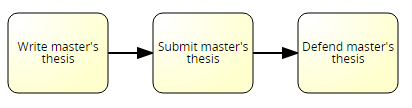
\includegraphics[width=.75\textwidth]{gfx/activity-introduction.png}
    \caption{The yellow boxes and their description are used in BPMN to describe an activity. The arrows denote the control flow in between.}
    \label{fig:activity-introduction}
\end{figure}

With the help of workflow management systems (WFMS), it became possible to embed and enforce these structured processes in an organization, making them traceable via the logs that these systems generated. 

Especially in the insurance and health-care sector, each case tended to be very different from the next \cite{hewelt2016}. This led to the notion that the course of a case strongly depends on the information contained inside it.

\subsection{Case Management}
In settings in which it is common to employ BPM, such as assembly line productions, there is little heterogeneity. As the latter increases, BPMN and other business process modeling notations result in complex and hardly understandable models and thus fail their purpose. As previously mentioned, this tends to occur in domains where the case trajectory is highly dependant on information contained inside it.

The fact that this type of process is data-driven led to the creation of the \textit{case folder} - a directory central to a case, describing its current state. In Case Management (CM), the process acts on the data contained inside this folder, making it have a direct impact on the course of a case. In contrast to BPM, the formalization of Case Management and the subsequent creation of modeling languages has only just begun. Notable developments include the Case Management Modeling Notation \cite{web:cmmn} as well as the Chimera approach \cite{hewelt2016}.
\todo[inline]{graphical illustration of case}

\subsection{Process Mining}
The logs generated through the users actions give rise to the discipline of Process Mining, which covers the three steps of model discovery, conformance checking and model enhancement \cite{Aalst2016}. They are enabled through the use of techniques from the area of Data Science, making it possible to understand Process Mining as the link between Data Science and Process Science as in \autoref{fig:process-data-science}. An excerpt from a log is depicted in figure \ref{fig:process-log}.

A major problem in this domain pose \textit{spaghetti} and \textit{lasagna} models. Such overly complex and unreadable models are mined from process logs that contain highly variable execution traces. Such logs often come from CM executions.

\begin{figure}
    \centering
    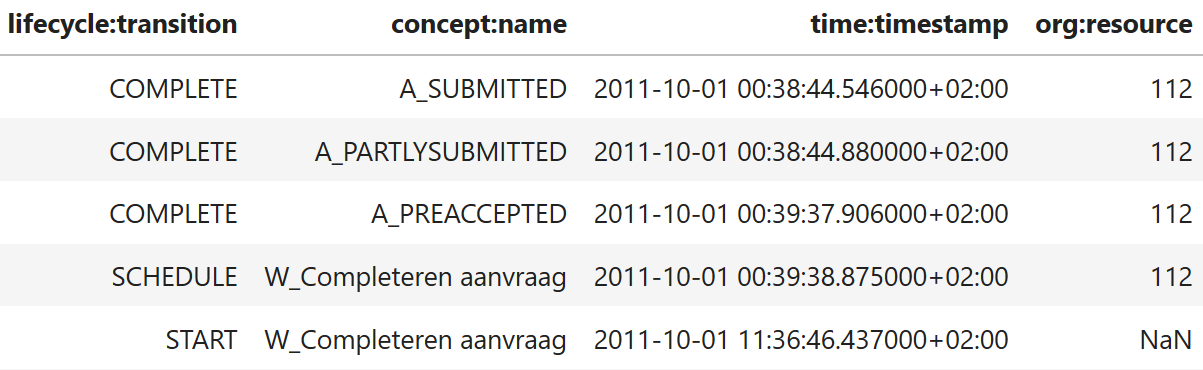
\includegraphics[width=\textwidth]{gfx/process-log}
    \caption{The first entries of an exemplary event log from a case from the BPIC 2011 dataset\cite{BPIC2011}. Each event is associated with data and the column \texttt{concept:name} corresponds to the activity title.}
    \label{fig:process-log}
\end{figure}

\subsection{Predictive Process Monitoring}
In parallel to this development, WFMS already permitted the unstructured execution of processes, empowering the user to make the best choice about which activity to do next. The knowledge to do so made him or her the \textit{knowledge worker}.
As Process Mining is concerned with data-driven process discovery and optimization only on offline data, a possibility to act on case developments in real-time is desirable. Commonly referred to as \textit{Predictive Process Monitoring} \cite{francescomarino2015, schoenig2018}, the application of predictive analytics on running and thus incomplete case logs fulfills this need. Connecting two subdomains of Process Science and Data Science, this is what sets it apart from Process Mining \autoref{fig:process-data-science}.

\begin{figure}
    \centering
    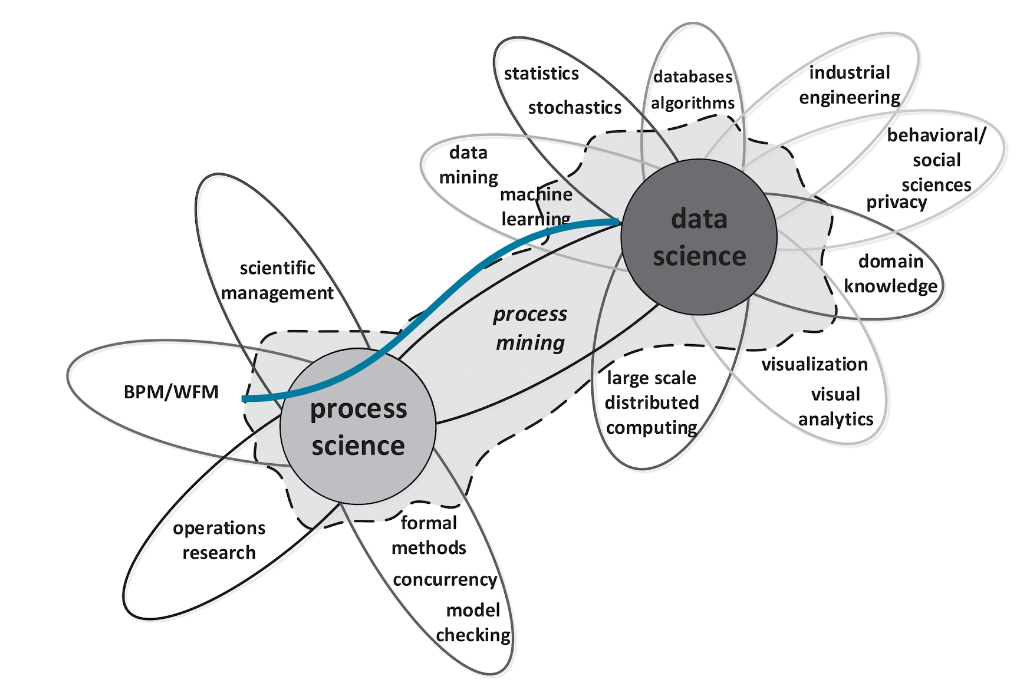
\includegraphics[width=\textwidth]{gfx/process-data-science.png}
    \caption{Process Mining can be understood as the bridge between Process Science and Data Science \cite[p.18]{Aalst2016}. The blue line symbolizes the subdomains that Predictive Process Monitoring brings together.}
    \label{fig:process-data-science}
\end{figure}

Instead of revolving around models, this discipline is concerned with predicting certain characteristics of the running case that lie in its future. This allows answering questions such as:

\begin{itemize}
    \item Will I still meet my service level agreement?
    \item Will we be able to deliver the package in within our 3-hour target?
    \item How long is this case still going to take?
    \item What is going to be the next step?
\end{itemize}

The answers to these questions can give case workers the opportunity to intervene if a case takes an unwanted course or might fail to meet KPI requirements. Furthermore, this approach only requires sufficient amounts of historical case executions, but no model. While it can certainly be a useful addition, it is not needed. 

%\begin{figure}
%	\centering
%	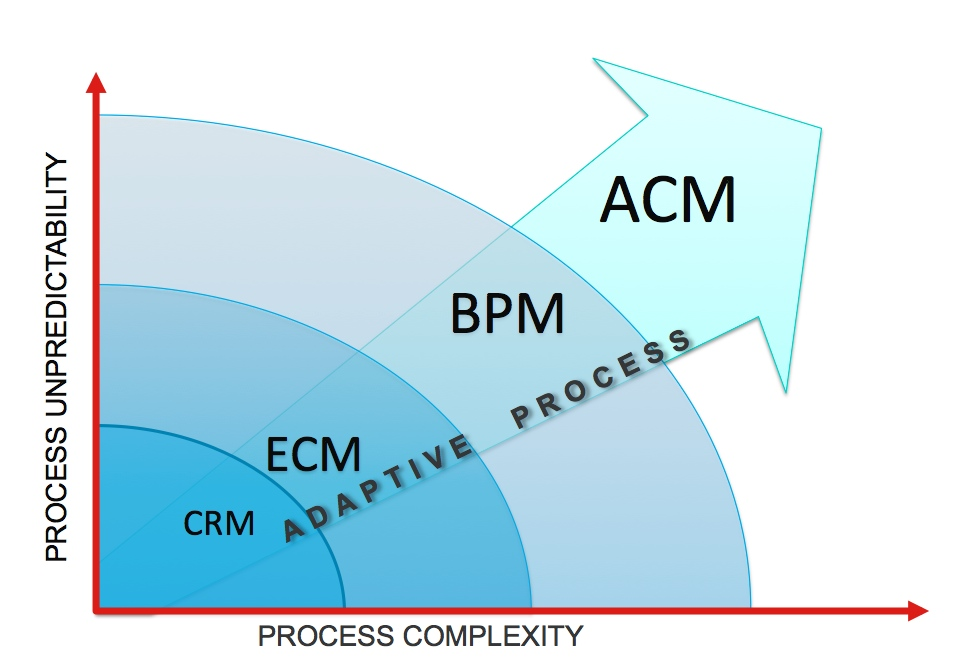
\includegraphics[width=\textwidth]{gfx/acm-reasoning}
%	\caption{https://acmisis.wordpress.com/what-is-adaptive-case-management-acm/}
%	\label{fig:why-acm}
%\end{figure}

\section{Predictive Modeling}
Predictive modeling is a process that uses data mining and learned statistical properties of the data, henceforth referred to as predictive models, to forecast outcomes. It is important to note that predictive models are unrelated to process models. This section shall introduce a common process for predictive model generation and frame a problem that is fundamental to the thesis: that of next-element predictions in a sequence.

\subsection{Predictive model development}
A predictive model takes in a number of \textit{features}, which are variables that are likely to influence the prediction of the \textit{target variable}. Features are sometimes also referred to as predictor variables.
These features are often \textit{engineered}, i.e. aggregated, or differently encoded to assist the model during learning.

The model itself can be chosen from a wide array of possibilities, such as linear regressions, decision trees, random forests, scalable vector machines (SVM) or neural networks (NN).

Once features and model are chosen, the model is \textit{trained} on the dataset. During this training phase, the model uses accuracy metrics to assess the quality of its predictions, learn the statistical properties of the data and adjust itself internally accordingly. Certain input parameters of the model are adjusted during this phase as well, an activity referred to as \textit{hyper-parameter tuning}. Training the model can be a very time-consuming task, unless appropriate hardware is used. Such hardware might be specially designed for model learning (i.e. Google's Tensor Processing Units) or a simple Graphics Processing Unit (GPU).

As predictors, model choice and hyper-parameters have a strong impact on model quality, these steps are frequently iterated upon, as Fayyad et al. discovered \cite{fayyad1996data}. The process for model development they discovered 20 years ago is illustrated in \autoref{fig:kdd_process} and as current as ever.

\begin{figure}
	\centering
	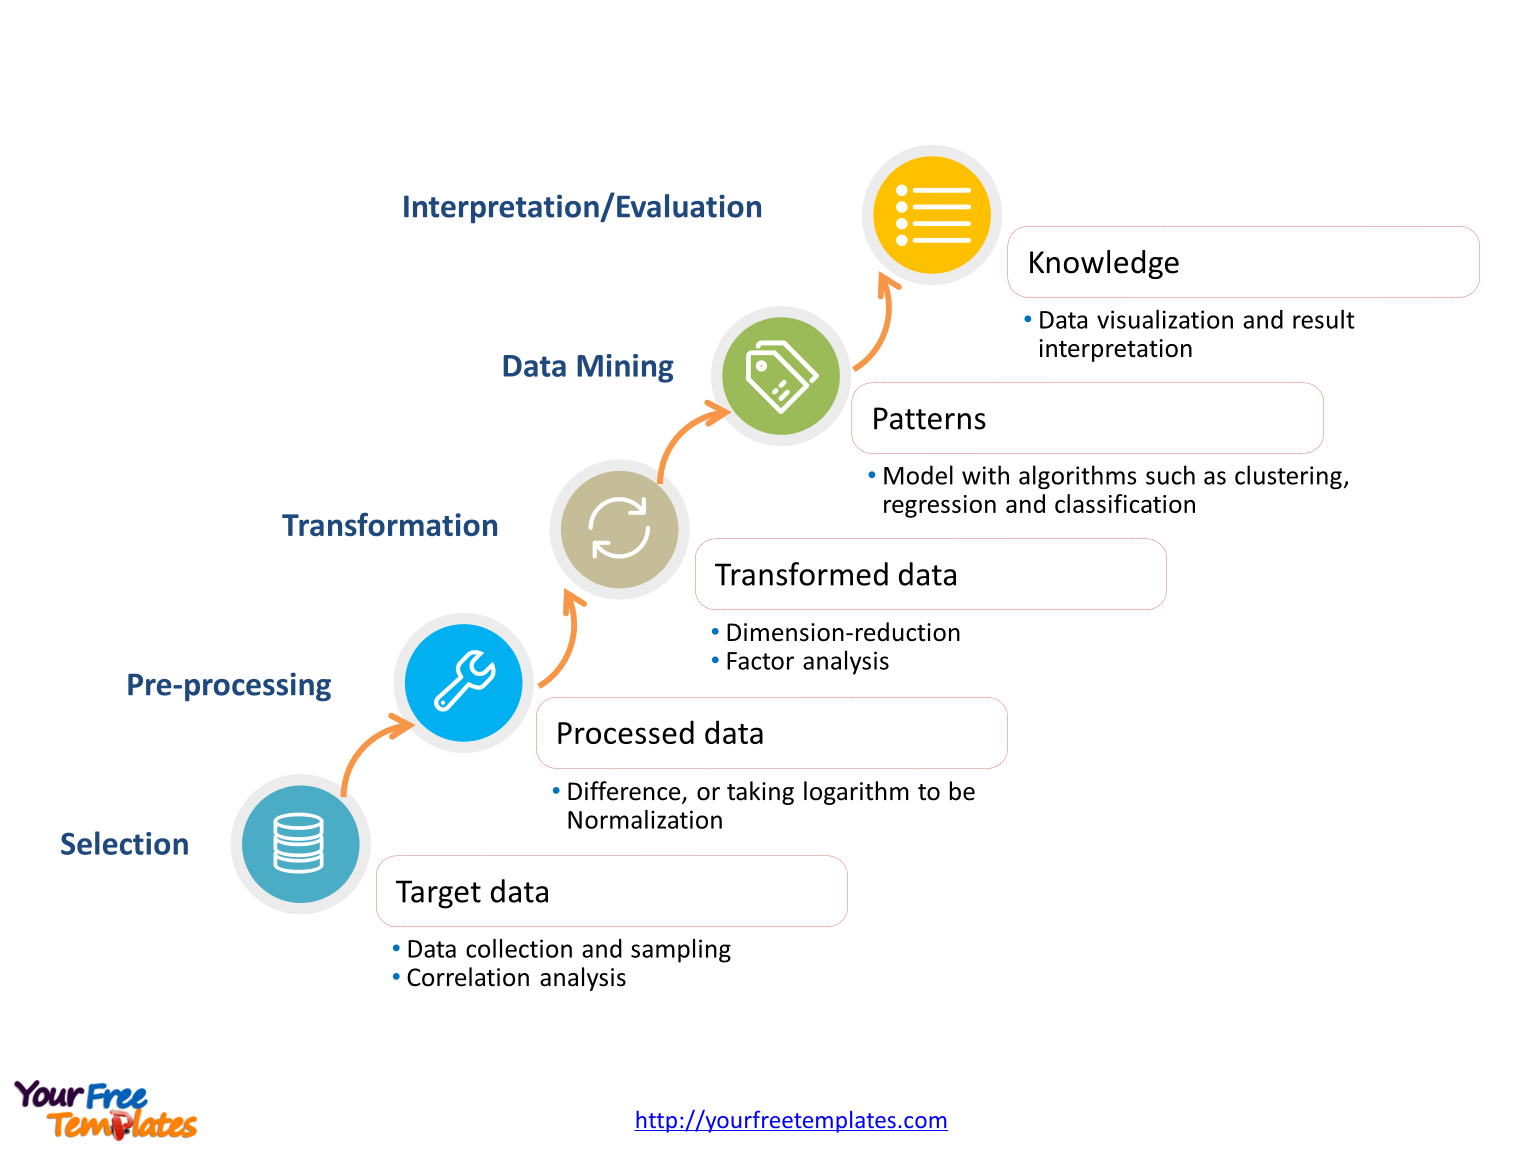
\includegraphics[width=\textwidth]{gfx/kdd_process}
	\caption{The process for \textit{Knowledge Discovery in Databases} as per Fayyad et al. \cite{fayyad1996data}.}
	\label{fig:kdd_process}
\end{figure}

\subsection{Sequence prediction}
In this section, a formal definition of sequences is presented, and then set in relation with the problem at hand\footnote{Definition adapted from \cite{pei2001prefixspan}}.  Let $I = \{i_1,i_2,...i_n\}$ be the set of all items. An \textit{itemset} is a subset of $I$. A \textit{sequence} is an ordered list of itemsets, such that in its notation $seq = \langle s_1s_2...s_l \rangle$, the following rule holds: $\forall\ 1 \leq j \leq l: s_j \subseteq I$. Then, $S$ defines the infinite set of all possible sequences. It is infinite because sequences can be arbitrarily long, with each itemset containing an arbitrary number of items.

Assuming that a a sequence can be finished, consider the database of completed sequences $DS$. Under the assumption of the Markovian hypothesis that "[...] the probability of each event depends only on the state attained in the previous event"\footnote{Gagniuc, Paul A. (2017). Markov Chains: From Theory to Implementation and Experimentation. USA, NJ: John Wiley \& Sons. pp. 1–235. ISBN 978-1-119-38755-8.}, a predictive model is be trained on this database to predict the next sequence $nseq$ or itemset $s_k$ of an incomplete sequence $seq_{inc}$:

\begin{equation}
\begin{split}
    predict(seq_{inc}) &= \widehat{nseq}\\ predict(seq_{inc}) &= \hat{s_k}\ |\ 1 \leq k \leq l
\end{split}
\label{eq:prediction-from-sequence}
\end{equation}

Sequence predictions are a common problem in the domains of machine translation and text generation. For example, the translation of the sentence \textit{"I am writing my master's thesis"} into the german sentence \textit{"Ich schreibe meine Masterarbeit"} can easily be mapped onto the notation previous described. With $I$ being the alphabet and punctuation marks and each itemset representing a single word, the input and target sequences could be noted as:

\begin{equation*}
\begin{split}
seq_{in} &= \langle<I>, < >, <am>, ... <thesis>\rangle\\
seq_{out} &= \langle<Ich> ... <Masterarbeit>\rangle
\end{split}
\end{equation*}

Referring to the \autoref{eq:prediction-from-sequence}, $seq_{in}$ can be understood as $seq_{inc}$ and $seq_{out}$ as $\widehat{nseq}$. This was an example of a classic \textit{sequence-to-sequence} prediction.

Next to this kind of prediction, there are also \textit{sequence-to-word} predictions, which can be used to generate text and even write simple novels.

However, the next itemset of a sequence need not be a word - it can also be an activity of a business process still running. The formal transfer of sequence prediction to business processes shall be presented in \autoref{sec:contribution}, as it is an important part of the contribution.

Predictive models such as random forests take inputs of fixed size. Unfortunately, sequences can be of arbitrary length, and thus the \textit{curse of dimensionality} also appears in context with this problem. To bring variable length inputs into a format that can be processed by predictive models (such as in \autoref{fig:process-log}), several data input formats have been invented. As their names suggest, these come from the domain of Natural Language Processing (NLP), but can easily be transferred to the problem at hand. These shall be briefly introduced in the following:

\subsubsection{Sliding Window}
\subsubsection{N-gram}
\subsubsection{Bag-Of-Words}
\subsubsection{Learned features, word2vec}
Strictly piecewise\\
subsequences, embedding
PrefixSpan

\section{Neural networks}
give insights into deep learning and neural networks 

follow explanation of colah.github.io

\subsection{RNN}
\subsection{LSTM memory}
\chapter{Related Work}\label{chap:related-work}
As this thesis brings together Predictive Process Monitoring with an approach from NLP, this chapter on related literature presents selected publications from both domains.

Publications related to Predictive Process Monitoring are presented in \autoref{sec:related-work-predictive-process-monitoring}, with the chapter ending in a detailed presentation of the two publications reimplemented for comparison. Similarly, \autoref{sec:related-work-sequence-prediction} presents other sequence prediction approaches from NLP and ends with in-depth information on a publication which we adapted for the use case at hand.

\section{Predictive Process Monitoring}\label{sec:related-work-predictive-process-monitoring}
We found that there are three types of prediction targets in current publications on Predictive Process Monitoring: constraint predictions, case-specific next-event predictions, and general next-event predictions without regard to a specific case. These three types will serve as subdivisions to this section.

\subsection*{Constraint predictions}
A constraint could be the delivery of a product within a given timeframe, or the total runtime of a case~\cite{weske2012business, francescomarino2015}.

Polato et al. make use of data attributes attached to events in their work for improving the prediction of the remaining time of business process instances~\cite{polato2014}. During feature engineering, their training data is enriched with information about possible other activities. With support vector regression (SVR) from the WEKA toolkit~\cite{web:weka} and default parameters, they are able to reach $6\%$ and $9\%$ mean absolute percentage error (MAPE) on two non-public datasets of 5000 and 1500 traces. While the authors criticize the use of non-public datasets, they also do not publish theirs nor their source code, making the results hard to compare.\\

Metzger et al. predict constraint violation of a case by comparing fundamentally different prediction models and combining them into an ensemble. The ensemble is tested with different voting mechanisms, e.g. majority voting or recall-orientation. They argue that late and precise or early and incorrect predictions are equally worthless for interventions and that predictions should stabilize as early as possible. They establish that after progressing $60\%$ to $85\%$ into the case, predictions become stable and precise.

Three approaches are used to predict constraint violations: constraint satisfaction, Quality-of-Service (QoS) violation checks and machine learning. The two former models use rules to predict a process outcome while the latter is a trained neural network. For it, Metzger et al. use the ANN implementation from the WEKA machine learning toolkit with a single hidden layer.

The authors are able to formulate rules for the two other models because the process at hand is very rigid and well defined: The Cargo 2000 process is a standard proposed by the International Air Transport Association (IATA)~\cite{metzger2015}. Two-thirds of their non-public dataset of 3942 traces and 56082 events were used for training and the remainder for testing.

While model ensembles can be expected to bring small accuracy improvements, they incur a lot of work and are typically only found in research~\cite{lessmannBADS}. Furthermore, we expect that the use an RNN on this simple process would have yielded a high accuracy than the stated $0.7$.\\

Francescomarino et al. organized predictive models in a clustered fashion~\cite{francescomarino2015} to predict predicate fulfillment. Having clustered the training data, one model was trained on each cluster. Then, to obtain a prediction, the cluster for a new data item needed to be found, and the corresponding model selected. Furthermore, the authors varied the probability threshold for accepting a prediction and measured how it affected the point in process progress at which the predictions become stable (similar to Metzger et al.). They refer to this characteristic as \textit{earliness}. Their approach, implemented as a ProM plugin called \textit{Predictive Process Monitoring}, uses k-means or DBSCAN to cluster the data and decision trees or random forests to make the prediction. It was tested on the BPIC11~\cite{BPIC2011} dataset and obtained accuracies of up to $0.9$.

Clustering improves tree-based models because it makes the training data more homogeneous. By using embedding layers, an ANN can cluster the data by itself, making a manual clustering unnecessary.

\subsection*{Case-specific next-event predictions}
Next-event predictions specific to a case allow answering the question "which activity comes next in this special case?" - the question that this thesis tries to answer with deep learning.\\

Huber~\cite{huber2015} gives an example of how a next-step prediction and recommendation system for case workers might look like. The system is prototypically implemented within CoCaMa, a case management application. Its predictions are produced as follows: After gathering the training data from various sources via an extract, transform and load (ETL) process, several \textit{Next Models} are constructed. There are four Next Models which use different data: timestamps, deadlines, decisions, and goals. The predictions from these individual models are combined by the recommender via weights to produce a recommendation. Huber uses decision trees from the WEKA~\cite{web:weka} machine learning toolkit to implement them. The system has been evaluated with 25 hand-made traces~\cite{huber2015}, which explains why high accuracies could not be obtained.\\

Next-event prediction without any machine learning is done by Böhmer et al. with a method rooted in heuristic analysis~\cite{boehmer2018probability}. The authors argue that the amount of trust that users put into ANN predictions is limited due to the fact that ANNs are not only computationally expensive but that their black-box nature makes their predictions and inner workings very hard to comprehend. As potentially large organizational changes could be made based on the predictions, the authors perceive it of importance to explain alternative futures which were not classified as being most probable and explain the aspects which motivated specific prediction results.
Böhmer et al. approximate trace similarities with the Damerau-Levenshtein method and a custom cost function. Using this method, they filter historic traces to produce a set of similar executions, and go on to mine probability distributions from it. The most probable behavior is used as the final next-event prediction~\cite{boehmer2018probability}. Additionally, they predict the timestamp of its execution. They evaluate their approach on the BPIC12 datase~\cite{BPIC2012} as well as a Helpdesk event log~\cite{Helpdesk}. On both datasets, they achieve an accuracy of $0.77$ for the next-event predictions.

While understanding the reasons for a prediction is important, forgoing black-box models completely could mean missing out on potentially higher accuracies~\cite{tax2018interdisciplinary}. With techniques such as LIME, predictions made by black-box models can be explained~\cite{ribeiro2016should}, albeit the computational power required is undeniably higher.\\

Klinkmüller et al. enrich their training dataset with features that encode subsequence occurrence~\cite{klinkmuller2018reliablemonitoring} to predict the next event in a trace based on its history, which they refer to as prefix. Doing so on a synthetic dataset, they are able to increase the accuracy of random forests in comparison to a baseline that is not using the engineered subsequence features. This approach is similar to that of Shibata et al.~\cite{shibata2016bipartite}, which is thoroughly examined in the next section. Furthermore, the authors find that training models on complete traces is preferable to the popular practice of trace truncation.\\

Francescomarino et al. also used LSTM networks to predict the next events of a case, and engineered features which indicate the presence of a loop~\cite{francescomarino2017}. To enhance the predictions further, they apply a compliance-checking logic on top of the predictions which leverages a-priori knowledge to rule out forbidden next events. The network is trained with windowed samples, and the following accuracies on these six datasets are obtained:
EnvLog~\cite{EnvLog}: $0.07$, HelpDesk~\cite{Helpdesk}: $0.816$, BPIC11~\cite{BPIC2011}: $0.276$, BPIC12~\cite{BPIC2012}: $0.408$, BPIC13~\cite{BPIC2013}: $0.516$, BPIC17~\cite{BPIC2017}: $0.439$

\subsection*{General next-event predictions}
General next-event predictions predict the next event in a stream of events, without specifying which case this event belongs to. Here, Evermann et al.~\cite{evermann2016} and Schönig et al.~\cite{schoenig2018} made contributions, which also build upon each other.

Evermann et al. remark the lack of research on next event predictions and have successfully demonstrated the applicability of LSTM neural networks in the context of predicting the next event in a stream of events. Using a neural network implemented with Tensorflow, precisions between $0.60$ to $0.90$ on the BPIC12 and BPIC13 datasets are achieved. Evermann et al. want their work to be understood as a "demonstration of the applicability of the approach and the potential for future work". The authors highlight that their work lacks the use of data attributes during model training.

Schönig et al.~\cite{schoenig2018} picked up on the last point and demonstrated on the BPIC dataset from 2017 that using data attributes complementary to the event names does increase prediction accuracy. Schönig et al. implemented their solution with Keras and trained it with stratified 5-fold cross-validation.
The data was pre-processed with one-hot encoding for categorical variables and min-max-normalization for continuous features. Also, the work demonstrates that an increasing number of included data attributes can improve accuracy~\cite[p.5]{schoenig2018}, without referring to any of their statistical properties. Their approach reaches accuracies around $0.90$, depending on its configuration. It is important to note, however, that neither Evermann et al. nor Schönig et al. predict the next event \textit{specific to a trace}, but the next event in the whole event stream without attribution to a case.

\begin{figure}
\centering
\subfloat[][Architecture used by Evermann et al.~\cite{evermann2016}.]{
    
\includegraphics[width=0.3\textwidth]{gfx/evermann-network-architecture.png}
    \label{fig:evermann-architecture}
}
\qquad
\subfloat[][Architecture used by Schönig et al.~\cite{schoenig2018}.]{
    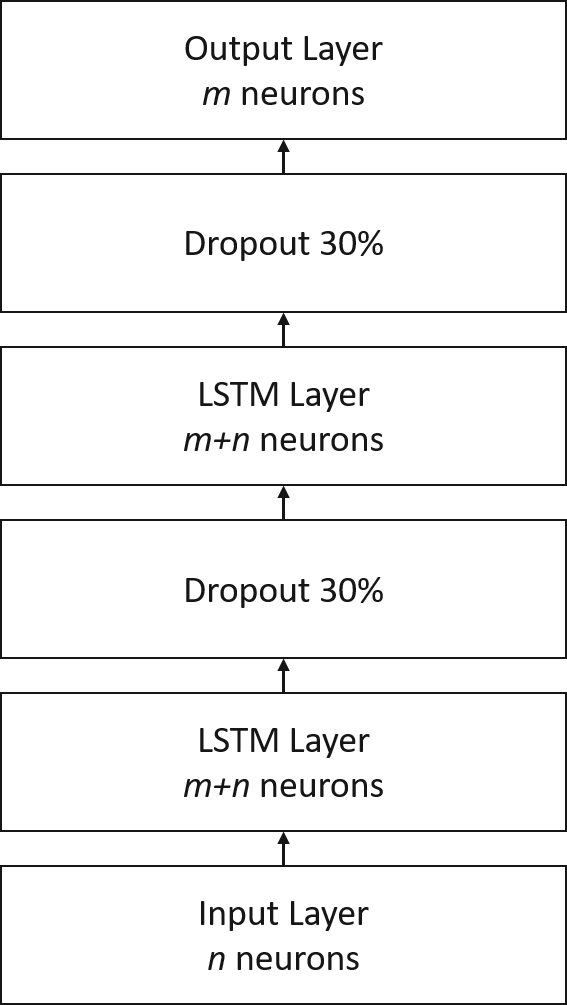
\includegraphics[width=0.3\textwidth]{gfx/schoenig-network-architecture.png}
    \label{fig:schoenig-architecture}
}
\caption[Overview of the reverse-engineered networks]{An overview of the reverse-engineered networks that are used as a comparison in this thesis. $n$ denotes the dimensionality of the input vector, and $m$ the number of output classes, including the end-of-sequence marker.}
\label{fig:benchmark-architectures}
\end{figure}

We take the works of Evermann et al. and Schönig et al. and reimplement them as direct comparisons to our adapted approaches as they were tested on BPIC data, their source code was made readily available and their authors were helpful in ensuring the correctness of our understanding. Furthermore, their approaches were fully based on neural-networks with little additional pre- or post-processing. In close collaboration with the two authors, their neural networks were reverse-engineered and also the architectures in \autoref{fig:benchmark-architectures} were confirmed to be correct. Both model the prediction task as a multi-classification problem.

Clearly, Evermann's architecture left an inspiring impression with Schönig, who decided to remove the Embedding layer and adapt unit counts and activation functions. In our conversation, Schönig argued that the Embedding was not needed, as the number of unique events was a lot lower than that of words in a text, for which Embeddings were originally developed. Where Evermann et al. used stochastic gradient descent (SGD) with a manual adaption of learning rate decay to $0.75$ after the 25th epoch, Schönig et al. use RMSprop with default values to optimize the network's loss. Furthermore, Schönig et al. fed the training data into their networks in a windowed fashion, contrary to Klinkmüller's suggestion that this might produce unstable results~\cite{klinkmuller2018reliablemonitoring}.

\section{Sequence prediction}\label{sec:related-work-sequence-prediction}
Sequence prediction deals with predicting the next element or next sequence from a given input, as explained in \autoref{sec:background:sequence-prediction}. It is rooted in NLP, and relevant publications are discussed in this section.\\

Attention is a fairly new development in the domain of ANNs, and it has been leveraged by Kokkinos et al. in a tree-structured neural network to classify sentiments in sentences~\cite{kokkinos2017structural}. In a detailed comparison with other works, their bipartite tree approach yields the highest accuracy on the Stanford Sentiment Treebank dataset. While the proposition of tree-structured Gated Recurrent Units (GRUs, a variant of LSTM units) and their use of attention forms the main contribution of this work, the authors make use of a bipartite network architecture and word embeddings as well. This gives further appeal to the idea of adapting the approach of Shibata et al, presented in the following.\\

In 2016, the International Conference in Grammatical Inference 2016 (ICGI) held a competition called SPiCE\ "about guessing the next element in a sequence"~\cite{web:spice}. It entailed making next-element predictions on twelve different datasets on which to make predictions for the next word. Most entries submitted to this competition made use of RNNs with LSTM cells to do so.\\

\begin{figure}
    \centering
    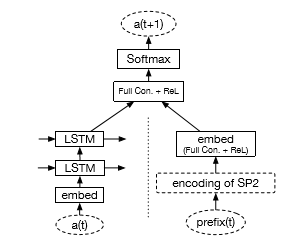
\includegraphics[height=.4\textwidth]{gfx/spice-winner-architecture.png}
    \caption{Neural network architecture of the winning submission at the SPiCE competition~\cite{shibata2016bipartite}}
    \label{fig:spice-winner-architecture}
\end{figure}

The winning submission by Shibata et al. uses a bipartite network architecture, training separate layers on different features of the same sentence. The results of these separate layers are then merged in the middle hidden layers to produce a single output~\cite{shibata2016bipartite}, as \autoref{fig:spice-winner-architecture} shows. Architectural similarities with Schönig et al. and Evermann et al. are especially prominent in the left part of Shibata's model.
While one-half of the layers are trained on the most recent word of the sentence, the other half is trained on the prefix of that word. As this prefix can be of any length, Shibata et al. propose a binary bag-of-words encoding, representing the states of an SP-2 automaton.

SP-$k$ languages are used to describe certain long-term dependencies through forbidden subsequences. For example, if $\langle a,b \rangle$ is forbidden, then no $b$ may ever occur after $a$. According to Heinz, who assisted Shibata, deterministic finite automatons (DFA) can also be used to characterize SP-$k$ languages, if the DFA states encode those subsequences of size $k-1$ present in the previous prefixes~\cite{heinz2010estimatingSP}. To make this concept more tangible, \autoref{tab:sp2-encoding} illustrates a small example. The authors argue that LSTMs are not completely understood yet and it has not been proven that they are fully capable of recognizing sequences, which is why these features should assist the network. To prove their point, they compare the SP-$k$ bipartite architecture with a basic one that is nearly identical to the one by Evermann et al. in \autoref{fig:evermann-architecture}. The performance differences between the two models are acknowledged as generally "slight", while the basic architecture performs "significantly worse on three problems".\\

\begin{table}[!htb]
    \centering
    \begin{tabular}{cclccccc}
        \hline
          &      &              & \multicolumn{5}{c}{SP-2 vector}\\
        t & a(t) & prefix(a(t)) & [a & b & c & d & e]\\
        \hline
        0 & a    & a            & [1 & 0 & 0 & 0 & 0]\\
        1 & d    & ad           & [1 & 0 & 0 & 1 & 0]\\
        2 & a    & ada          & [1 & 0 & 0 & 1 & 0]\\
        3 & c    & adac         & [1 & 0 & 1 & 1 & 0]\\
        4 & d    & adacd        & [1 & 0 & 1 & 1 & 0]\\
        \hline
    \end{tabular}
    \caption[SP-2 feature vector example]{Prefixes encoded with SP-2. As $t$ progresses, more and more single-item subsequences ($k-1=1$) are marked as occurred. The alphabet is $I=\{a,b,c,d,e\}$. This example is taken from Shibata et al. ~\cite{shibata2016bipartite}.}
    \label{tab:sp2-encoding}
\end{table}

\chapter{Sequence prediction for running cases}
\label{chap:taking-inspiration}
While a number of works have demonstrated the applicability of LSTM neural networks to Predictive Process Monitoring, most have left out a perspective on the sequence prediction problem from Natural Language Processing (NLP). In this chapter we outline how we take inspiration from sequence prediction in NLP, and thus add to improvement area 3 from \autoref{sec:intro:contribution}.

We establish the connection between processes and sequences by connecting their definitions in \autoref{sec:contrib:case-sequence-understanding}. This provides the underpinning for introducing two NLP-inspired approaches for predicting the next activity in a case. These are presented in \autoref{sec:contrib:sp2-inspiration} and \autoref{sec:contrib:pfs-inspiration}.

\section{Understanding a trace as a sequence}\label{sec:contrib:case-sequence-understanding}
The definition for sequences presented in \autoref{sec:background:sequence-prediction} and the definition of traces in \autoref{sec:log-structure} will be connected in this section to make it clear how events can be understood as itemsets.

Both a trace $\#_{trace}(c)$ from a case $c$ and a sequence $seq$ are already defined in a very similar manner:
\begin{equation*}
\begin{split}
seq           &=  \langle s_1,s_2\cdots s_l \rangle\ |\ \forall\ 0 \leq j \leq l: s_j \subseteq \mathscr{I}\\
\#_{trace}(c) &= \langle e_1, e_2, e_3 \dots, e_n \rangle
\end{split}
\end{equation*}

Any itemset consists of items $s = (i_1, i_2 \cdots i_n)$ with $i \in \mathscr{I}$. Events are made up of attributes that are accessed via the $\#$ operator.
In a first step, attributes are defined as items, so that any possible value from any attribute can be understood as an item:

$$\mathscr{I} = \{\#_{a}(e)\ |\ c \in L\wedge e \in \#_{trace}(c) \wedge a \in attrs(e)\}$$

In a second step, a schema is applied to the itemsets. Without it, the itemset that should represent an event could consist e.g. only out of timestamps, as $s \subseteq \mathscr{I}$ does not place any restrictions on the content of $s$.
The schema also provides the tabular format required for machine learning applications, and is introduced as a direct mapping from event $e$ to itemset $s$:

$$ s = (i_1, i_2 \cdots i_n)\ |\ i_i = \#_{attrs(e)[i]}(e) $$

The definition places each item on a specific place in the itemset, depending on the index in the attribute list $attr(e)$. Still, the original condition $s \subseteq \mathscr{I}$ hold true, and now permits sequence prediction on traces.

\section{Adapting a competition submission}\label{sec:contrib:sp2-inspiration}
Shibata et al.'s bipartite network architecture has shown outstanding performance in the SPiCe competition~\cite{web:spice}. Under the assumption that a case exhibits properties similar to sentences, we adapt it for use in the business process domain.

\begin{figure}[!htb]
    \centering
    
\includegraphics[width=0.8\textwidth]{gfx/sp2-network-architecture.png}
    \caption{SP2 network architecture and its dimensions}
    \label{fig:sp2-architecture}
\end{figure}

\autoref{fig:sp2-architecture} displays the adapted network architecture from Shibata et al., and we shall describe the changes we made in the following.

The Embedding layers were completely removed. Above the SP-2 feature input layer, the embedding layer was replaced with a fully-connected layer. The reason for the removal is as follows: Shibata et al. predicted the next word in a sentence based on the preceding words, and as such, the itemsets that they used consisted of a single item: a word~\cite{shibata2016bipartite}. We aim to predict the next activity based on the preceding events, and as shown in the previous section, the event-itemsets consist of multiple items which represent different attributes.
Embedding layers require dictionary-encoded input of a single item, which is a problem when multiple items belong together~\cite{goldberg2014word2vec}. An alternative to the removal would have been the concatenation of the outputs of one Embedding layer per attribute type. We decided against this due to the relatively small amount of available training data and the increased computational overhead.

The model uses $n$ units on the first input layer, denoting the dimensionality of the input vector with its encoded activity name, timestamps and other event attributes. It puts out the next activity in one-hot encoded form through $m$ units, thus modelling the task as a multi-classification problem.

In contrast to Evermann et al. and Shibata et al., the number of units $m+n$ in the hidden layers is a function of the input unit count and the output unit count. This follows general advice not to introduce bottlenecks in the hidden layers by using fewer units than required in the output layer~\cite{web:techniques-in-convnets,szegedy2016rethinking}. Furthermore, dropout layers have been introduced to prevent overfitting.

The SP-2 features are to be engineered based on the activity names, as the name of the next activity is also the prediction target. Shibata et al. also encoded the history of the prediction target in their implementation~\cite{shibata2016bipartite}. The SP-2 features are fed in higher up on the right side of the tree, passing through a ReLU-activated, fully-connected layer, before concatenation with the LSTM output. Finally, the concatenated vectors are processed by fully-connected layers, with the commonly used Softmax activation function producing the classification.

\section{Encoding subsequence occurrence}
\label{sec:contrib:pfs-inspiration}
Klinkmüller et al. compared different feature representations and found that sub-trace occurence features help the model cover a broader variety of relationships~\cite{klinkmuller2018reliablemonitoring}. While they found this to be true for random forests, we want to investigate the applicability of such features for LSTM neural networks since we established the similarity of traces and sequences. While the results from Francescomarino et al. are discouraging~\cite{francescomarino2017}, another network architecture could make a difference.

Since SP-2 features already encode history and subsequence encodings do the same on a higher level of abstraction, we take the SP2 model architecture and inject different features in place of the SP-2 features. Said features and the corresponding architecture will henceforth be referred to as PFS, as illustrated in \autoref{fig:pfs-architecture}. The acronym PFS originates from the word PrefixSpan, which is the name of the algorithm used in \autoref{chap:evaluation} to mine the subsequences.

\begin{figure}[ht]
    \centering
    
\includegraphics[width=0.8\textwidth]{gfx/pfs-network-architecture.png}
    \caption{PFS network architecture and its dimensions}
    \label{fig:pfs-architecture}
\end{figure}

\chapter{A process prediction training Framework}\label{chap:training-framework}
During development of the models, we realized that there are highly divergent understandings regarding the batch construction for next-element predictions with sequences. We believe that these different understandings strongly impact the reproducibility of prediction approaches. Therefore we present here a framework that enables researchers to compare the different understandings and easily try out new model architectures. In doing so, we hope to contribute to Area 1 and 2 in \autoref{sec:intro:motivation}.

In this chapter, we show a selection of possible batch construction strategies in \autoref{sec:contrib:input-formatting} and the underlying technical reasons. Finally, we present the training framework in \autoref{sec:contrib:training-framework}.

\section{Contrasts among batching strategies}\label{sec:contrib:input-formatting}
We implemented the SP2 and PFS models as well as the comparison models using Python and the Keras neural networks API. While doing so, a wide range of recommended possibilities to train the models were noted in relevant publications and on online platforms.\\

Some recommend sliding window approaches, while others deem this against the concept of LSTM cells. Especially Klinkmüller et al. argue against it: "[...]the popular strategy of cutting traces to certain prefix lengths to learn prediction models for ongoing instances is prone to yield unreliable models"~\cite{klinkmuller2018reliablemonitoring}. Again others argue that padding and truncating sequences to the same length makes training faster and does not affect accuracy. The batch size strongly affects convergence properties of any neural network, making it an important hyper-parameter to tune~\cite{keskar2016large}. No guidelines how to sort traces into batches were found. We believe that the understanding of the merits of each batch construction strategy can be of general value to any application of sequence prediction.\\

Keras' implementation of LSTM is stateful \textit{during} a batch, and resets the cell state $C$ before the next batch~\cite{web:keras}. This is configurable, but for the sake of simplicity, it is advisable to keep related timesteps inside a single batch. Translated to traces, this means keeping a trace completely inside a batch. A Keras LSTM layer requires input data to be formatted in a three-dimensional array of fixed size for every batch. Each dimension has a defined meaning:

$$(n_{samples}, n_{timesteps}, n_{features})$$

Each sample contains a number of timesteps $n_{timesteps}$ containing a number of features $n_{features}$. $n_{features}$ is constant, as it represents the feature vector dimensions. For each sample, the Keras LSTM layer cells maintain a separate state, meaning that several traces can be trained on simultaneously~\cite{web:keras-lstm-state}. As the batches themselves do not need to have the same dimensions, this definition opens up a range of possibilities to construct batches. We highlight four of them in the following paragraphs. To the best of our knowledge, these have not been compared in this context yet.\\

First and easiest, one trace can be trained per batch. This fulfills the requirement of constant dimensions since only a single sample is used.

Second, \textit{some} traces can be trained inside a single batch. This is possible if all traces inside the batch have the same number of timesteps, i.e. have the same length. The number of samples and timesteps may vary between batches. A look at \autoref{fig:bpic2011-length-distribution} reveals a power-law distribution of trace lengths. Because of this, grouped batching could bias the model toward the long tail of the distribution, as longer and fewer traces are put into batches of their own.

\begin{figure}[ht!]
    \centering
    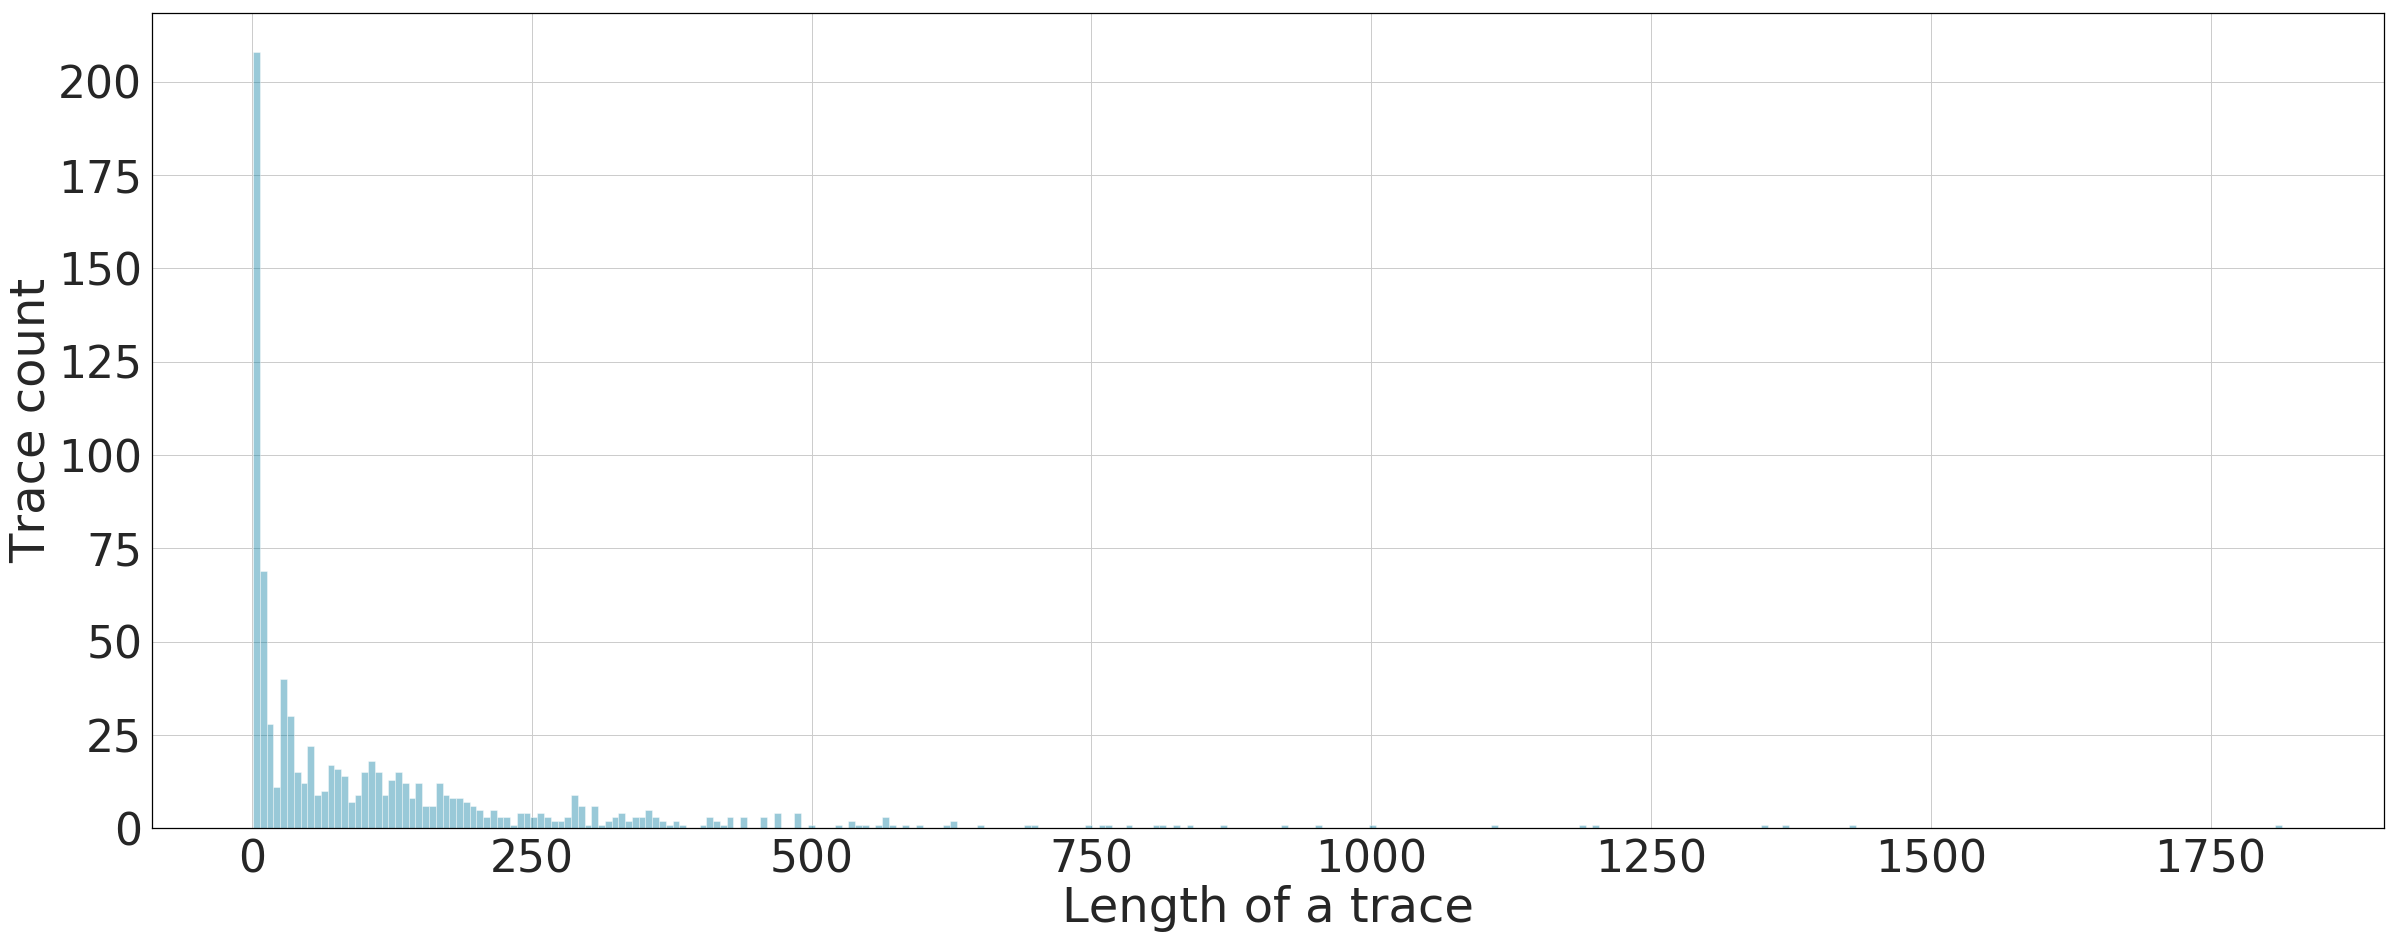
\includegraphics[width=.9\textwidth]{gfx/frequency-distribution.png}
    \caption{Distribution of trace lengths in BPIC11}
    \label{fig:bpic2011-length-distribution}
\end{figure}

Third, there is the possibility of padding the number of time-steps in a sequence to the same length and using a Masking layer to then filter out the padded values during training~\cite{web:keras}. The padding length is dictated by the maximum trace length and may incur a large memory overhead if it is a large outlier value like in BPIC11.

Fourth and finally, there is also the possibility to split the trace into samples by sliding a window along it. This results in $l-w+1$ samples for a trace of length $l$ and a window width $w$. Taking \autoref{tab:sliding-window} in \autoref{sec:background:feature-engineering} as an example, the window would be two timesteps wide. While this approach solves the problem of unequal sample lengths and facilitates batch construction, the model can only use a maximum of $w$ timesteps per sample for training and might lose potential long-term dependencies. As both Evermann et al.~\cite{evermann2016} and Schönig et al.~\cite{schoenig2018} use this format and it directly opposes the findings of Klinkmüller et al.~\cite{klinkmuller2018reliablemonitoring}, we investigate it. Furthermore, we are convinced that a windowed training data format misses out on LSTM potential.\\

The four batching strategies are labeled in the order of the preceding presentation for easier reference in the next chapter, where they are evaluated:
\begin{itemize}
\item\textbf{Individual}: One trace per batch
\item\textbf{Grouped}: Same-length traces in one batch
\item\textbf{Padded}: Padded-to-length traces
\item\textbf{Windowed}: Windowed samples, as used by Evermann and Schönig
\end{itemize}

\section{A next-event predictive model training framework}
\label{sec:contrib:training-framework}
We realize that making different process prediction approaches comparable is not only a technical but also a data-related challenge - no established benchmarking datasets for Predictive Process Monitoring exist yet.
To mitigate this situation, we designed a software framework that helped us compare the sixteen total model-batching-strategy combinations on a variety of datasets in an extensible way. We want to make this framework accessible to future researchers to facilitate model development and sharing of implementations.\\

\begin{figure}
    \centering
    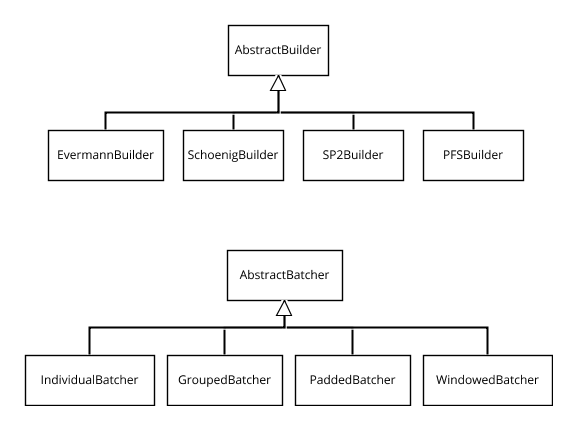
\includegraphics[width=\textwidth]{gfx/training-framework-classes.png}
    \caption[UML diagram of the framework classes]{Unified Modeling Language (UML) diagram of the abstract base class inheritance structure of Builders and Batchers}
    \label{fig:trainig-framework-classes}
\end{figure}

The proposed framework provides a simple training frontend and integrates two concepts: Builders and Batchers. As \autoref{fig:trainig-framework-classes} shows, the two concepts are introduced as abstract base classes from which the actual model and batching strategy implementations are derived.\\

\noindent\textbf{Builders} construct Keras models and also define the structure of the training and test data. This is important as models may not only have one input layer but two or more. These pre-formatted data sets are not structured into batches yet. One such Builder is implemented for every model type by inheriting from the abstract base class \verb=AbstractBuilder=.\\

\noindent\textbf{Batchers} take the pre-formatted data sets and structure them into batches. For each batching strategy, a class inherits from the abstract base class \verb=AbstractBuilder=.\\

\noindent The \verb=model_runner= frontend ties these two concepts together with training logic and provides a basic command-line interface as \autoref{fig:framework-frontend} shows. It allows for flexible training of a model with a specific Builder and a specific Batcher. It also permits placing the training process on a specific GPU and defining the output directory for the model and performance measurement files. The training algorithm also implements early stopping, of which the thresholds can be configured via a configuration file.\\

With the help of this framework, future researchers only need to subclass \verb=AbstractBuilder=, and can directly evaluate the model performance on any given dataset without having to implement the whole training environment. By simply sharing their Builder and Batcher implementations, it will be much easier for other researchers to reproduce findings. The framework and detailed documentation is hosted under \href{https://github.com/flxw/nitro4ppm}{github.com/flxw/nitro4ppm}.

\begin{figure}
\centering
\begin{verbatim}
usage: model_runner.py [-h] [--gpu GPU]
                       [--output OUTPUT]
                       {evermann,schoenig,sp2,pfs}
                       {padded,grouped,individual,windowed}
                       datapath

The network training framework script for Felix Wolff's master's thesis!

positional arguments:
  {evermann,schoenig,sp2,pfs}
                        Which type of model to train.
  {padded,grouped,individual,windowed}
                        Which mode to use for feeding
                        the data into the model.
  datapath              Path of dataset to use for training.

optional arguments:
  -h, --help            show this help message and exit
  --gpu GPU             CUDA ID of which GPU the model
                        should be placed on to
  --output OUTPUT       Target directory to put model
                        and training statistics
\end{verbatim}
\caption[CLI frontend for the framework]{The \texttt{model\_runner} command-line frontend for the training framework}
\label{fig:framework-frontend}
\end{figure}

\chapter{Evaluation}\label{chap:evaluation}
Through the use of the framework described in the previous chapter, we evaluate four different algorithms for next-activity prediction side-by-side: Two implementations that mimic Evermann et al. and Schönig et al, and the PFS and SP2 approaches presented in \autoref{chap:taking-inspiration}. For each model, we will analyze the four different approaches for structuring the training data for performance differences from \autoref{chap:training-framework}.

First we justify our choice of datasets in \autoref{sec:dataset-choice}. As we follow the KDD process, we then lead through the data preprocessing and transformation phases in \autoref{sec:eval:data-preprocessing} and \autoref{sec:eval:data-transformation}. The latter section also covers the strategy used to engineer the SP-2 and PFS features. Then, the test setup and the used training strategy is presented in \autoref{sec:eval:test-setup}, followed by the set of criteria by which we judge the results in \autoref{sec:eval:criteria}. Finally, the chapter ends with the presentation in \autoref{sec:eval:results} and discussion of the results in \autoref{sec:eval:discussion}. Used and relevant technologies are highlighted in each sections.

\section{Choice of dataset}
\label{sec:dataset-choice}
In \autoref{sec:intro:contribution}, we criticized the great variety of datasets used to evaluate approaches in Predictive Process Monitoring. While we can not establish a standard, we ensure comparability of our results to a variety of works by evaluating the four models on eight datasets in total, coming from the following sources:

\begin{itemize}
    \item BPIC11, an event log from cases in a Gynaecology department a Dutch Academic Hospital~\cite{BPIC2011}
    \item BPIC12, an event log for loan and overdraft applications from a Dutch Financial Institute~\cite{BPIC2012}
    \item BPIC15 provides logs by five Dutch municipalities. It contains all building permit applications over a period of approximately four years. It is divided into one dataset per municipality, referred to as BPIC15-1 to BPIC15-5 in the following~\cite{BPIC2015}
    \item Helpdesk Log, TODO TODO TODO
\end{itemize}
\todo[inline]{Check out the helpdesk log and see if it's worth it...}

We picked the three BPIC datasets as we believe that they cover a spectrum of process complexity. The least complex end of it is marked by BPIC12, which covers a loan application process from a financial institution with a small variance in trace length and a very small number of different activities. The complex end is marked by BPIC11, which covers patient treatments in a hospital. This results in logs of longer traces and an especially high number of distinct activities. BPIC15 resides relatively in the middle of the two, as \autoref{tab:dataset-characteristics} indicates.

While process models were easily mined for BPIC12\footnote{Citation needed}, they were more complex for BPIC15~\cite{van2015benchmarking}, and barely obtained for BPIC11. Furthermore we take the increasing number of distinct activities to be a measure of complexity.

Furthermore, these datasets allow us to compare our findings to the following works, which also worked on next-element predictions. When comparing, it is important to differentiate between the works that focused on case-specific predictions like us and those that focused on whole event streams:

\begin{itemize}
    \item Predicting the next element in a stream, not specific to a case
    \begin{itemize}
        \item BPI12: Tax et al.~\cite{tax2018interdisciplinary, tax2017}
        \item BPI12: Evermann et al.~\cite{evermann2016}
    \end{itemize}
    \item Predicting the next element for a specific case
    \begin{itemize}
        \item BPI12: Böhmer et al.~\cite{boehmer2018probability}
    \end{itemize}
\end{itemize}

\begin{table}[]
\centering
\begin{tabular}{lrrrrrrr}
\textbf{Dataset} & \textbf{min TL} & \textbf{max TL} &  \textbf{mean TL} & \textbf{\# Traces} & \textbf{\# Events} & \textbf{\# Activities} \\
\hline
\textbf{BPIC11} & 1 & 1 814 & 131.49 & 1 143 & 150 291 & 524\\
\textbf{BPIC12} & 3 & 96 & 12.56 & 13 087 & 164 506 & 23\\
\textbf{BPIC15-1} & 2 & 101 & 43.55 & 1199 & 52 217 & 398\\
\textbf{BPIC15-2} & 1 & 132 & 53.31 & 832 & 44 354 & 410\\
\textbf{BPIC15-3} & 3 & 124 & 42.35 & 1409 & 59 681 & 383\\
\textbf{BPIC15-4} & 1 & 116 & 44.91 & 1053 & 47 293 & 356\\
\textbf{BPIC15-5} & 6 & 154 & 51.10 & 1156 & 59 083 & 389\\
\end{tabular}
\caption{Properties of the traces contained in the used datasets. TL abbreviates trace length.}
\label{tab:dataset-characteristics}
\end{table}

\section{Data preprocessing}
\label{sec:eval:data-preprocessing}
In the first step of the KDD process~\cite{fayyad1996data}, the data is preprocessed to eliminate generally known properties that hinder machine learning model performance. In our case, this encompassed three steps for all datasets:

\begin{enumerate}
    \item Drop all columns which exhibit zero entropy, i.e. which contain only a single value
    \item Eliminate features which correlate strongly. To account for categorical correlation, the bias-corrected version of Cramér's~V~\cite{bergsma2013bias} is used.
\end{enumerate}

In step 1, one column was dropped in BPIC11 and two were dropped in BPIC17.
In step 2, the bi-directional results in \autoref{fig:BPIC11-correlation-heatmap} from Cramér's V revealed that the variables \texttt{Producer code}, \texttt{Activity code} and \texttt{Specialism code} correlate strongly with many others in the BPIC11 dataset. Thus, these were dropped. As evidenced in \autoref{fig:BPIC12-correlation-heatmap}, the BPIC12 dataset with its small number of features did not require any removals. In the BPIC17 dataset, \texttt{EventID} and \texttt{OfferID} were removed for being identifiers, and \texttt{Action} for its perfect correlation with \texttt{concept:name}. The correlation measurements are on display in gdskjl
\todo[inline]{create table with features, and indicate which ones were removed}

The activities described above were conducted in JupyterLab notebooks~\cite{web:jupyter}, where Anaconda~\cite{web:anaconda} was used to create a stable development environment. The OpyenXes~\cite{web:opyenxes} library proved to be especially useful for parsing the raw XES logs from BPIC.

\section{Data transformation}
\label{sec:eval:data-transformation}
Having removed unneeded features, the remaining ones were encoded following standard practice. Each numerical feature $x$ was normalized with values specific to each trace using the min-max method:

$$normalize(x) =
\begin{cases}
\frac{x-min(x)}{max(x)-min(x)} & \text{if } min(x) \neq max(x)\\
1 & \text{otherwise}
\end{cases}
$$

Categorical features without ordinal properties, which were all of them, were encoded using one-hot encoding if possible. In the case of the input for Evermanns model, the concatenation of activity name and resource ID was encoded with dictionary encoding, as demonstrated in his paper~\cite{evermann2016}.

\subsection*{SP-2 feature engineering}
For every trace, SP-2 features mark whether an activity has occured yet. Thus, these features are engineered in an iterative fashion, as \autoref{lst:sp2-generation} outlines. For every trace, a new data frame \texttt{sp2\_df} is created and the occurence of the first activity is marked inside it. Now, a loop begins over the remaining steps, where each previous row inside \texttt{sp2\_df} is copied into the currently indexed row and the presence of the current activity is marked. This repeats itself until the trace has been processed completely.

\begin{listing}[ht]
\begin{minted}{python}
# Dataframe initialization with zeroes
sp2_df = pd.DataFrame(columns=activity_labels,
                      index=range(0,len(t)),
                      dtype=np.bool)
for col in sp2_df.columns: sp2_df[col].values[:] = 0

# mark first occuring SP-2 
cname = "{0}{1}".format(sp2_prefix, t[target_col][0])
sp2_df[cname].values[0]  = 1

# copy over values from last row and
# set activity labels accordingly
for i in range(1,len(t)):
    first_activity_name = t["concept:name"].iloc[i]
    col = "{0}{1}".format(sp2_prefix,first_activity_name)
    
    sp2_df.values[i] = sp2_df.values[i-1]
    sp2_df[col].values[i] = 1
\end{minted}
\caption{Generating SP-2 features for a single trace \texttt{t} and a specific target column \texttt{target\_col}.}
\label{lst:sp2-generation}
\end{listing}

\subsection*{Sub-sequence feature engineering}
The sub-sequence features for the PFS model were created with the help of the \textit{prefixspan-py} library~\cite{web:prefixspan-py}. As \autoref{lst:pfs-mining} shows, the library greatly facilitates obtaining closed sub-sequences ranked by support, returning a two-dimensional array of sub-sequences, with one array per sub-sequence. The sequences are mined from the entirety of traces.

\begin{listing}[ht]
\begin{minted}{python}
prefixspan_traces = PrefixSpan(encoded_traces)
closed_sequences = prefixspan_traces.topk(25, closed=True)
\end{minted}
\caption{Obtaining closed sequences using the \textit{prefixspan-py} library.}
\label{lst:pfs-mining}
\end{listing}

After mining the sequences, a loop is executed for every trace, shown in \autoref{lst:subsequence-feature-creation}. For each index \verb=i= it is checked whether any of the mined subsequences starts at that position. This is checked by peeking ahead of \verb=i= for the length of the subsequence. As in the case of the SP-2 features, the occurence of a subsequence is marked with a boolean flag from the row that it occured in onwards.

\begin{listing}[ht]
\begin{minted}{python}
subseq_df = pd.DataFrame(columns=subseq_labels,
                         index=range(0,len(t)),
                         dtype=np.bool)
subseq_df[:].values[:] = False
activity_codes = t[target_col].map(event_to_int)
tlen = len(t)

for i in range(0, tlen):
  # loop through all subsequences
  for subseq_idx, subseq in enumerate(ps):
    if tlen <= i+len(subseq): continue
            
    # check if subseq takes place in the following steps
    subsequence_found = True
    j = 0
    
    while subsequence_found and j < len(subseq):
      if subseq[j] != activity_codes[j+i]:
        subsequence_found = False
        j += 1

    # if subseq took place, subsequence_found is still true
    if subsequence_found:
      subseq_df.values[j+i:,subseq_idx] = True
\end{minted}
\caption{Enriching a trace \texttt{t} with sub-sequence features by detecting those that are contained inside it.}
\label{lst:subsequence-feature-creation}
\end{listing}

\subsection*{Target construction}
For each itemset $i_t$ at a given timestep $t$, the prediction target $a_t$ was constructed. While the itemset could also contain data attributes, the prediction target solely consisted of the activity name. For the target of the last $t$ of a trace, a marker for denoting the end of the sequence, \verb=EOS=, was introduced.
As the goal is to predict the next activity, the column containing this information needed to be identified in the data. For all three datasets, this turned out to be \verb=concept:name=.

\section{Test setup}
\label{sec:eval:test-setup}
To conduct the experiments, Docker containers were built with the development Anaconda environment inside them~\cite{web:docker}. Using a version of Docker for GPU applications running on NVIDIA hardware~\cite{web:nvidia-docker}, each network-batch-formatting combination was trained and evaluated on a single NVIDIA K80 GPU of the HPI FutureSOC Lab~\cite{web:fsoc}. The complete source code used for evaluation is publicly available on GitHub at \href{https://github.com/flxw/master-thesis-code}{flxw/master-thesis-code}.\\

All datasets were split into training and test sets of complete traces. While $25\%$ of the traces were used for validation and testing, the remaining $75\%$ were used for training purposes. The sets were shuffled and stratified to contain an approximately similar distribution of trace lengths.

Each model implementation was trained successively with each data formatting variant on a single GPU. A model was saved when its validation loss, calculated on the test set, hit a new record low. If the validation loss did not improve for 10 epochs, the training was interrupted. This is commonly referred to as early stopping. \autoref{tab:training-setup} illustrates information about the training setup of the networks side-by-side. As Evermann et al. made use of a version of Tensorflow that is deprecated as of the time of writing, our implementation in Keras can only be understood as an approximation. Evermann's implementation of an "unrolled LSTM" can only be approximated in Keras.

\begin{table}[ht!]
    \centering
    \begin{tabular}{lcccc}
        \textbf{Network}   & \textbf{Evermann} & \textbf{Schönig} & \textbf{SP2} & \textbf{PFS}\\
        \hline
        \textbf{Optimizer} & SGD\footnote{SGD stands for Stochastic Gradient Descent. Additionally setting the learning rate decay to $0.75$ at the $25^{th}$ epoch.} & \multicolumn{3}{c}{RMSprop} \\
        \textbf{Loss}      &\multicolumn{4}{c}{Categorical crossentropy}\\
        \textbf{Weight initializer} & Zeros & None & \multicolumn{2}{c}{Glorot normal}\\
        \textbf{Epochs}    & 50 & 100 & 150 & 150\\
        \textbf{Features}  & \makecell{Activity +\\Resource} & \multicolumn{3}{c}{All usable data attributes}\\
    \end{tabular}
    \caption{Used hyper-parameters for each model, with the number of epochs to be understood as the maximum number of epochs, as training may stop early}
    \label{tab:training-setup}
\end{table}

\begin{table}[]
\centering
\begin{tabular}{c|rrrr}
Dataset & Individual & Grouped & Padded & Windowed \\
\hline
BPIC11    & 1 & & 7 & 1054\\
BPIC 12   & 1 & & 103 & 939\\
BPIC 15-1 & 1 & & 727 & 365\\
BPIC 15-2 & 1 & & & 316\\
BPIC 15-3 & 1 & & & 414\\
BPIC 15-4 & 1 & & & 334\\
BPIC 15-5 & 1 & & & 420\\
\end{tabular}
\caption{Batch sizes for the different datasets and batching strategies}
\label{tab:batch-sizes}
\end{table}

\section{Evaluation criteria}
\label{sec:eval:criteria}
The following three metrics are the focus in the evaluation of the sixteen model-formatting combinations:

\begin{enumerate}
    \item\textbf{Accuracy} - The share of correct next-activity predictions.
    \item\textbf{Resource consumption} - The amount of time and memory required during training.
    \item\textbf{Stability} - Whether the prediction accuracy changes as the trace progresses.
\end{enumerate}

While the first two criteria target the general usability of each model, the last one permits making a judgment about the stability of the predictions. It is inspired by the works of Francescomarino et al.~\cite{francescomarino2015} and Klinkmüller et al.~\cite{klinkmuller2018reliablemonitoring}. This allows better insights into how prediction accuracy develops over time, and facilitates building trust in the model, as indicated in the introduction of the thesis.

\section{Results}\label{sec:eval:results}
The three aforementioned criteria were applied to each model-batching combination on each dataset, and the results are presented in this section. By evaluation criterion, we go through the measurements. Most of the corresponding figures can be found in the Appendix, due to space reasons. \autoref{tab:network-info} lists dimensions which can have an impact on performance and will be referred to throughout the following subsections.

\begin{table}[htb!]
\centering
\begin{tabular}{lcccc}
\textbf{Dataset} & \textbf{Evermann et al.} & \textbf{Schönig et al.} & \textbf{SP2} & \textbf{PFS}\\
\hline
\hline
\textbf{BPIC11} & 1 & \makecell{n=655\\m=625} & \makecell{n=655\\m=625} & \makecell{n=655\\m=625\\ l=25} \\
\hline
\textbf{BPIC12} & 1 & \makecell{n=655\\m=625} & \makecell{n=655\\m=625} & \makecell{n=655\\m=625\\ l=25} \\
\hline
\textbf{BPIC17} & 1 & \makecell{n=655\\m=625} & \makecell{n=655\\m=625} & \makecell{n=655\\m=625\\ l=25} \\
\end{tabular}
\caption{Input and output vector dimensionalities for each dataset}
\label{tab:network-info}
\end{table}

\subsection*{Accuracy}
The overall accuracy is a good indicator of the prediction performance of a sequence-prediction model. In this section we will go over the model performances per batching strategy and explain the results. In \autoref{fig:max-accuracies-bpic2011} to \autoref{fig:max-accuracies-bpic2015-5}, the model performances per dataset are presented, grouped by batching strategy. The plots make apparent that only three models perform well consistently and that all react very differently to each batching strategy.

Looking at the performance of the EVM model across all datasets, it is evident that it is consistently outperformed. Its performance on the BPIC12 datasets represents an exception. We trace this lack of performance back to the application of an Embedding layer, which we suspect to require more data than included in most datasets to improve its internal data representation. The performance jump on the BPIC12 dataset corresponds nicely to the small number of activities and large number of traces in \autoref{tab:dataset-characteristics}, which helps the Embedding learn better.

Unsurprisingly, the individual batching strategy often results in slightly worse accuracies than the grouped batching strategy, with the exception of the BPIC12 dataset. We trace this back to the frequent adjustment of weights that might lead the loss optimization into local minima. In the trace length distributions in \autoref{appendix:trace-length-distributions}, the explanation for the high accuracy on BPIC12 with the individual batching strategy can be found. As this dataset has the highest number of traces and a relatively even distribution of lengths, the batches become too large, leading to lost optimization opportunities. With this knowledge, the strategy should be enhanced to split batches if they exceed a certain size threshold.

The padded strategy leads to consistently good results throughout the datasets and only loses accuracy on the BPIC11 datasets where the training set had to be shrunk because traces exceeded the length threshold.

While the batching strategies that provide the whole history to the model consistently see the SCH, SP2 and PFS models on par with at most $0.1$ difference, the windowed batching strategy leads to very different results depending on the dataset and the model. With the window size set to three, the model does not have many timesteps to learn from in any given sample. However, this loss of information does not impact the SP2 model. We assume that its SP-2 features encode the history that is cut away and thus help it come close to the general maximum accuracy of the dataset with the exception of BPIC11.

\begin{figure}
    \centering
    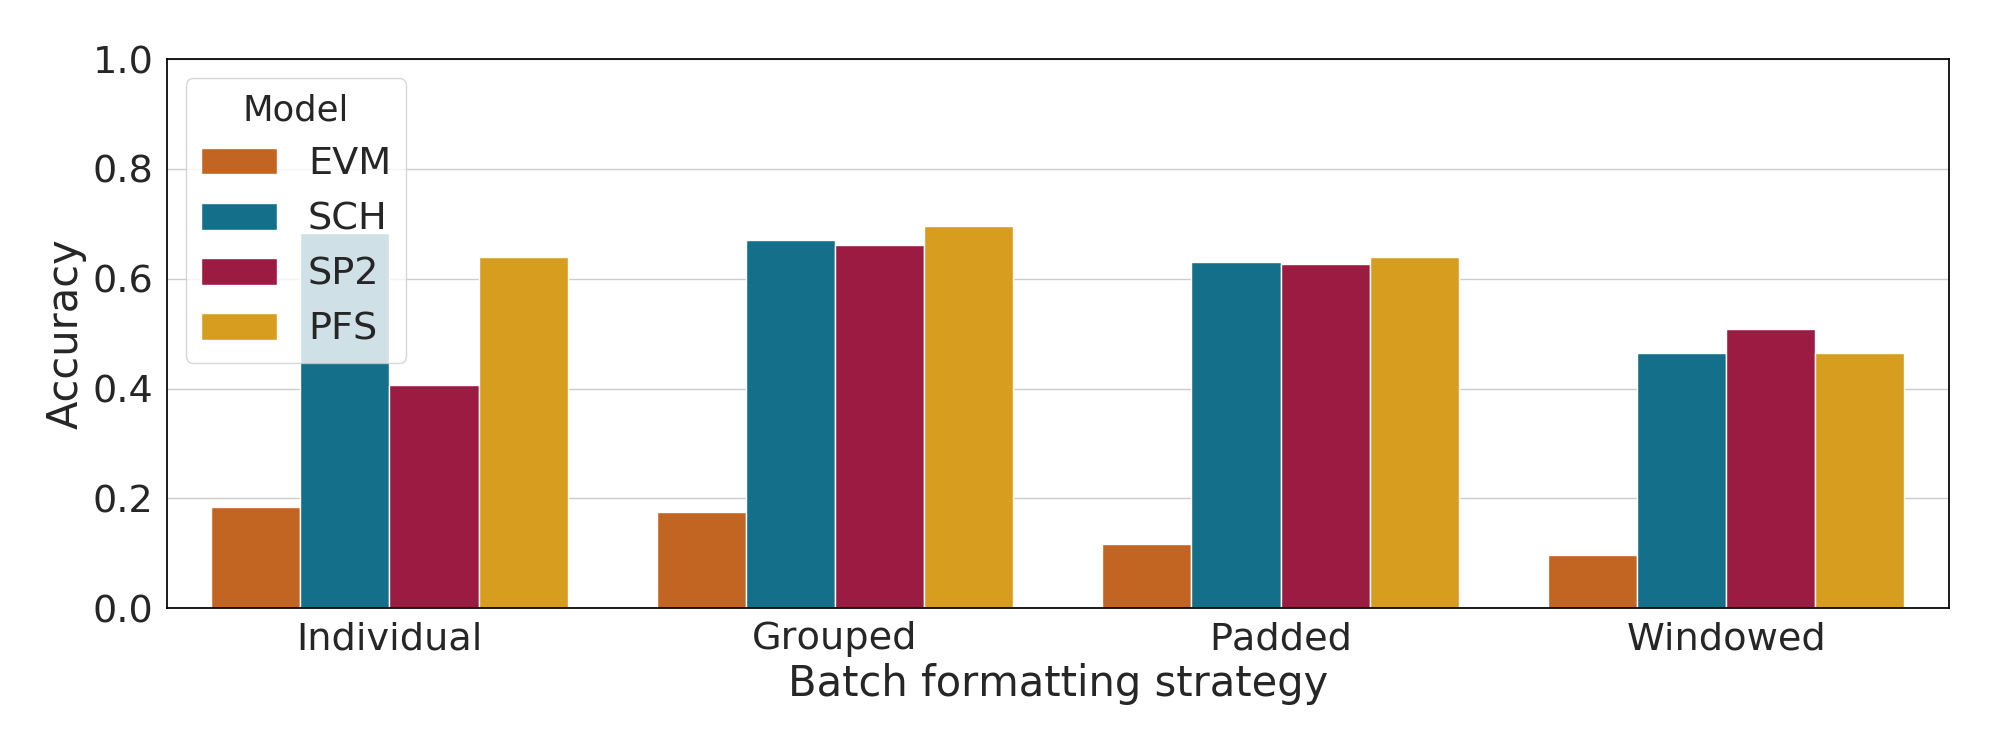
\includegraphics[width=\textwidth]{gfx/bpic2011/accuracies.png}
    \caption{Best accuracies obtained on the validation set on the BPI11 data}
    \label{fig:max-accuracies-bpic2011}
\end{figure}
\begin{figure}
    \centering
    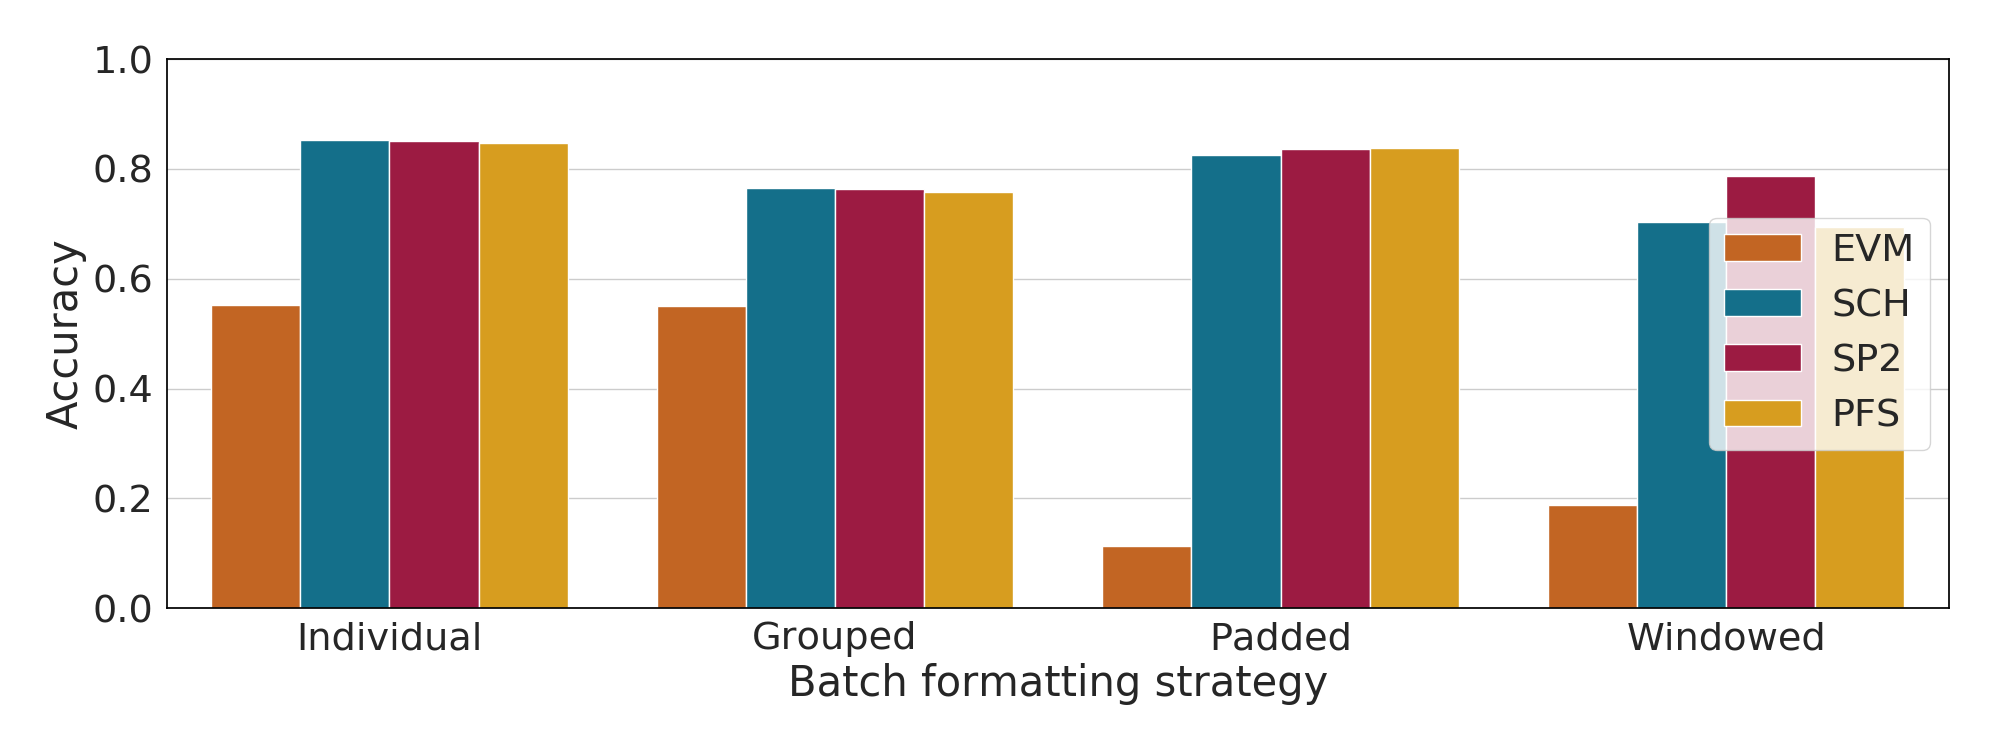
\includegraphics[width=\textwidth]{gfx/bpic2012/accuracies.png}
    \caption{Best accuracies obtained on the validation set on the BPI12 data}
    \label{fig:max-accuracies-bpic2012}
\end{figure}
\begin{figure}
    \centering
    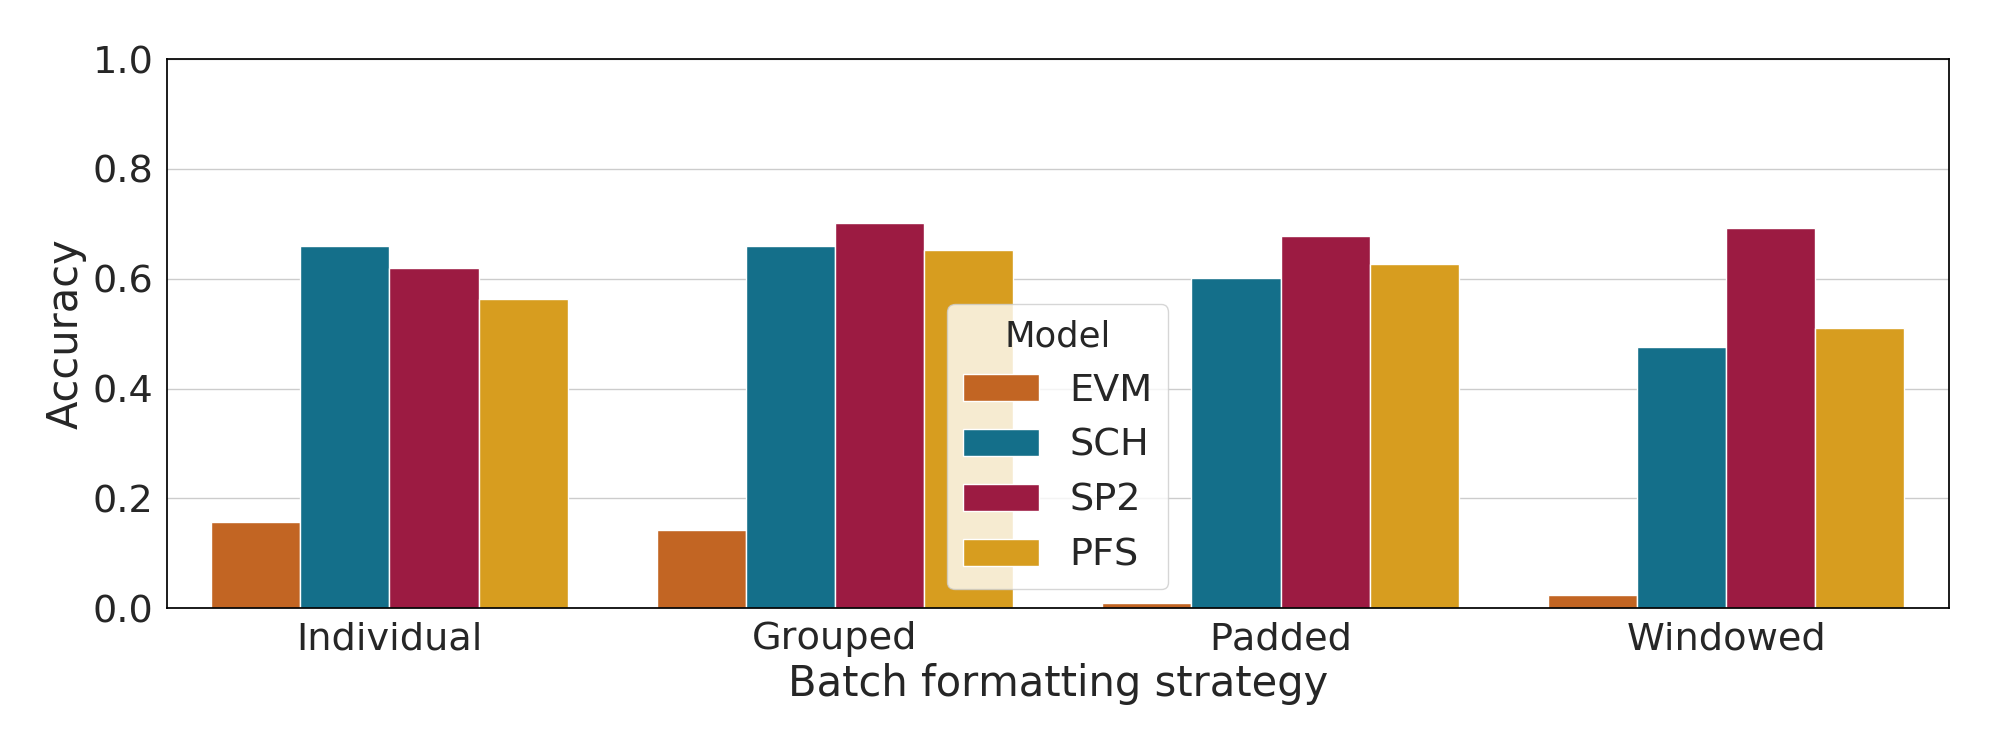
\includegraphics[width=\textwidth]{gfx/bpic2015_1/accuracies.png}
    \caption{Best accuracies obtained on the validation set on the BPI15-1 data}
    \label{fig:max-accuracies-bpic2015-1}
\end{figure}
\begin{figure}
    \centering
    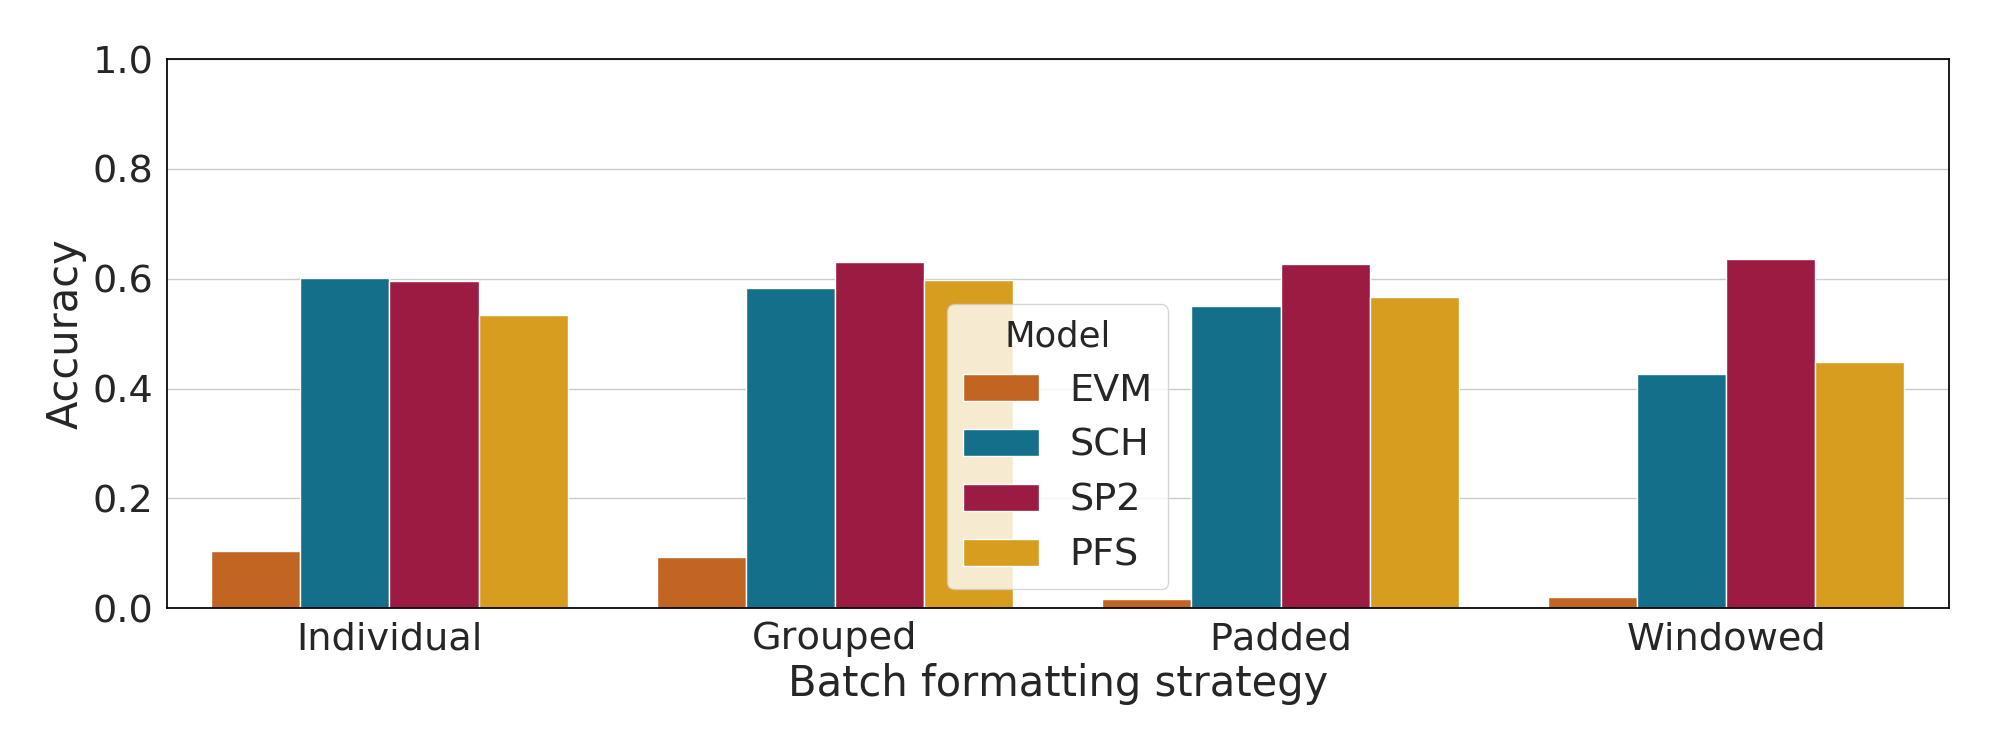
\includegraphics[width=\textwidth]{gfx/bpic2015_2/accuracies.png}
    \caption{Best accuracies obtained on the validation set on the BPI15-2 data}
    \label{fig:max-accuracies-bpic2015-2}
\end{figure}
\begin{figure}
    \centering
    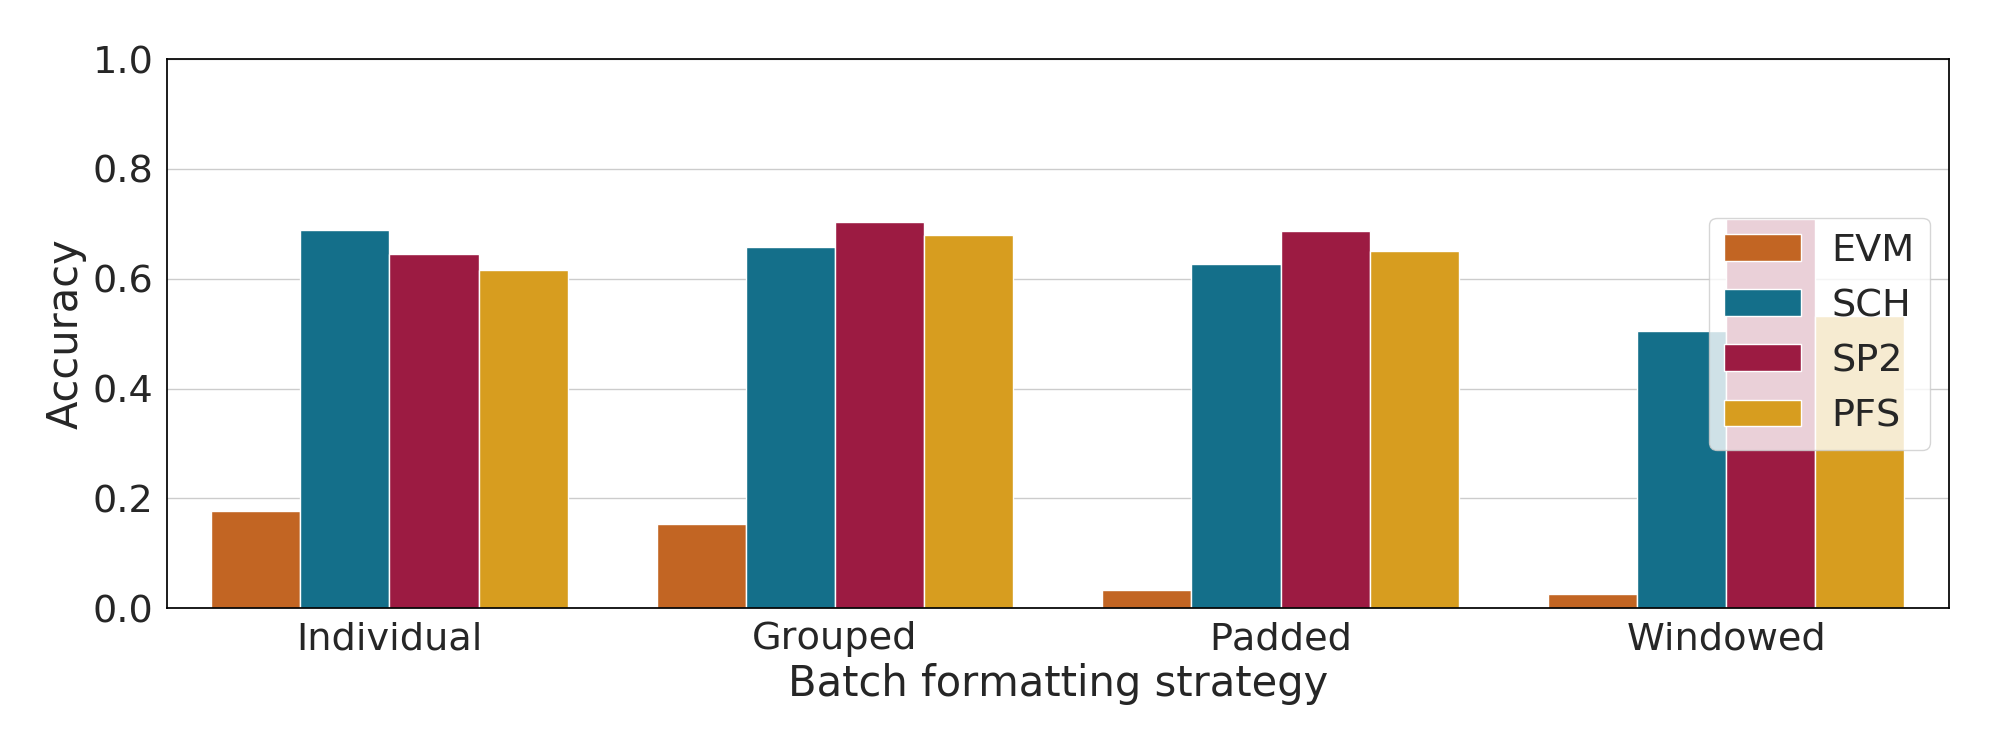
\includegraphics[width=\textwidth]{gfx/bpic2015_3/accuracies.png}
    \caption{Best accuracies obtained on the validation set on the BPI15-3 data}
    \label{fig:max-accuracies-bpic2015-3}
\end{figure}
\begin{figure}
    \centering
    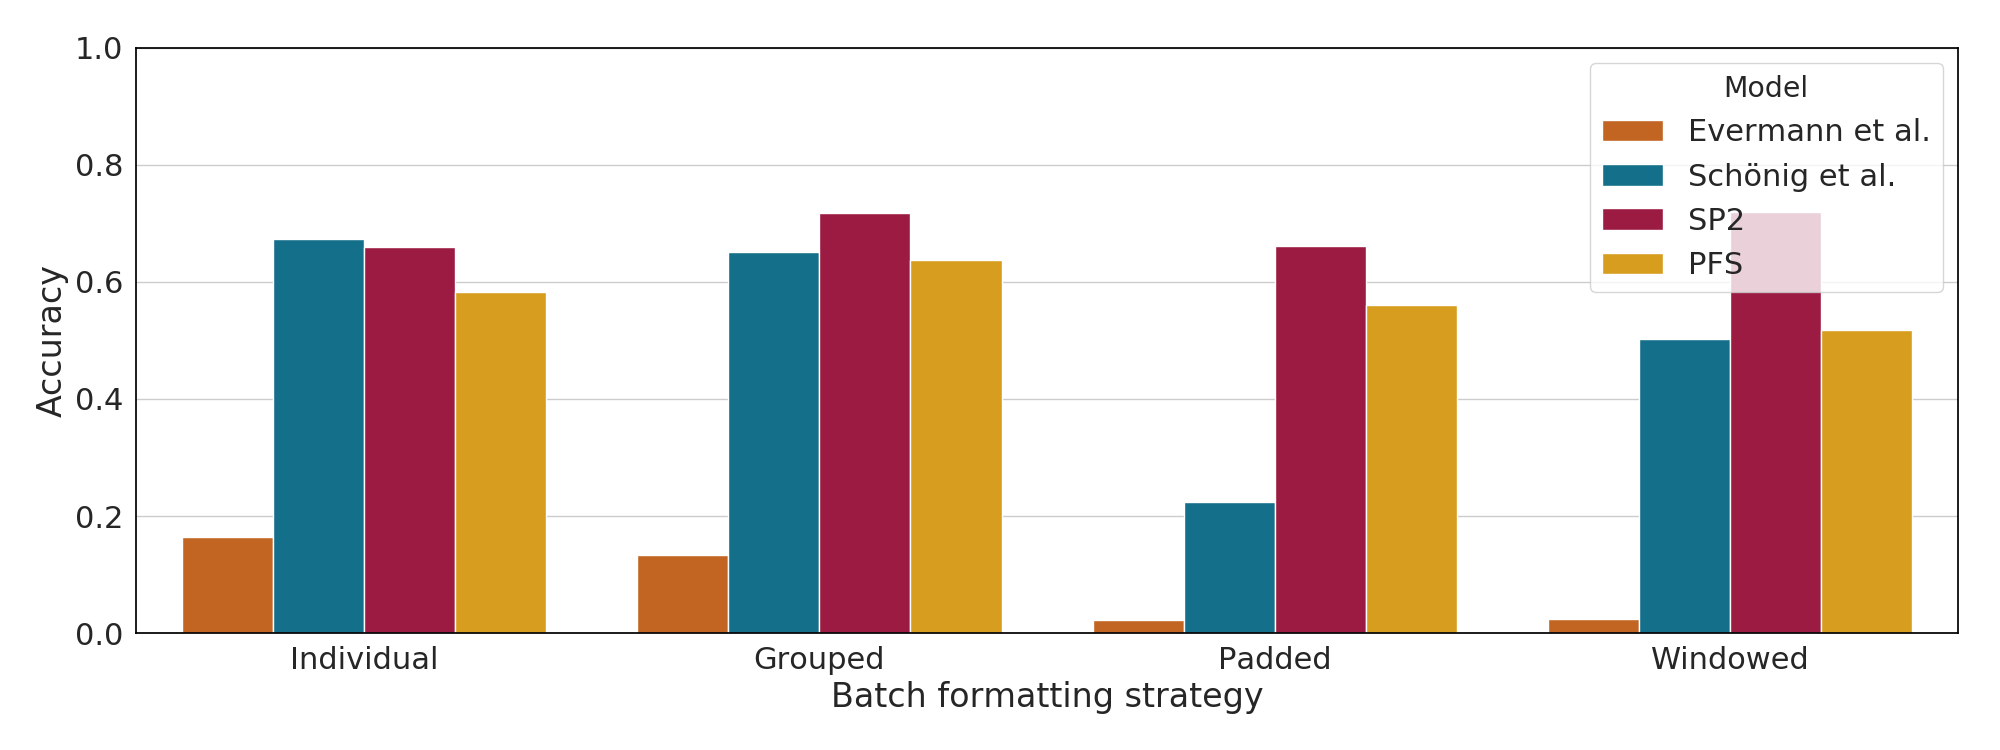
\includegraphics[width=\textwidth]{gfx/bpic2015_4/accuracies.png}
    \caption{Best accuracies obtained on the validation set on the BPI15-4 data}
    \label{fig:max-accuracies-bpic2015-4}
\end{figure}
\begin{figure}
    \centering
    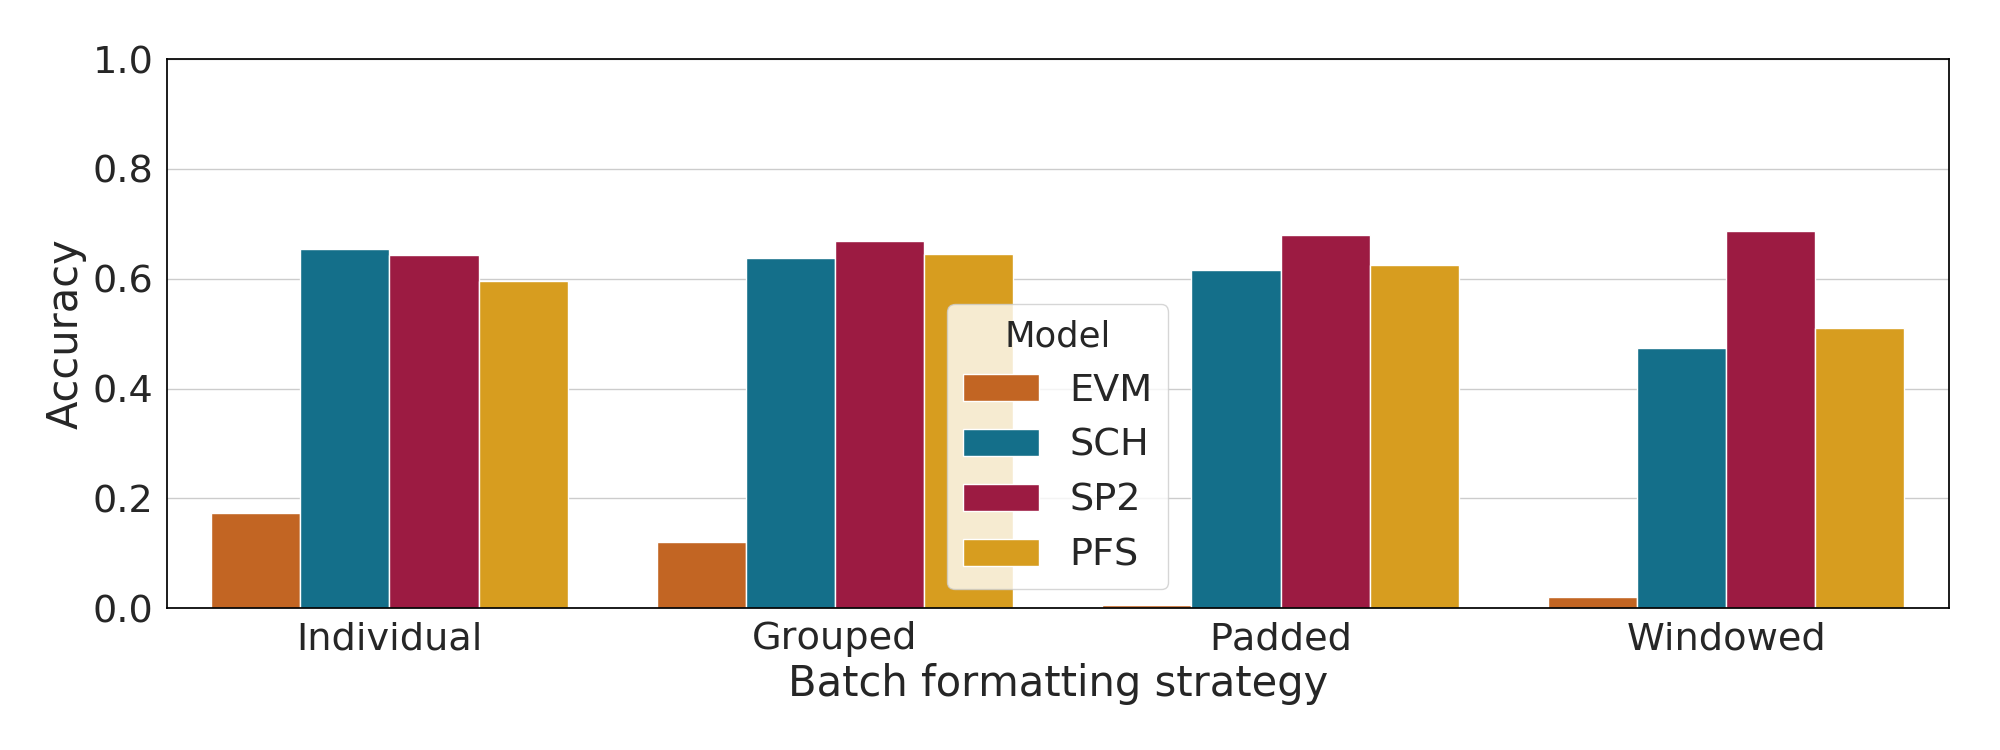
\includegraphics[width=\textwidth]{gfx/bpic2015_5/accuracies.png}
    \caption{Best accuracies obtained on the validation set on the BPI15-5 data}
    \label{fig:max-accuracies-bpic2015-5}
\end{figure}
\FloatBarrier

\subsection*{Training times}
The batch size is an important hyper-parameter, and since it directly corresponds to the number of weight adjustments per epoch, it also impacts the time that the training of an epoch requires. \autoref{fig:BPIC11-training-timings} to \autoref{fig:BPIC15-5-training-timings} illustrate the mean time required for training a model for an epoch, grouped by batching strategy.
In this section we will go over the training times per batching strategy and explain the results.

Unsurprisingly, the individual batching strategy leads to the longest epochs overall. With regard to the dataset characteristics in \autoref{tab:dataset-characteristics}, it becomes apparent that this strategy causes hundreds of weight adjustments per epoch.

The grouped batching strategy leads to significant reductions in training times, depending on how diverse the trace lengths are. \autoref{tab:dataset-characteristics} explains why the reduction is not as big with BPIC11: It exhibits up to 1814 different lengths, while the other datasets only exhibit $5\%$ to $10\%$ of this number.

With the padded strategy it is possible to overcome the limit imposed by trace lengths and construct batches out of any number of traces. This makes it easier to optimize the batch size, and can thus lead to faster training times. That this does not always lead to better accuracies was shown in the previous chapter, as e.g. this strategy leads to lost samples on BPIC11.

Finally, the windowing strategy is the fastest by far. It produces a constant number of timesteps and allows for arbitrary batch sizes.

\begin{figure}
    \centering
    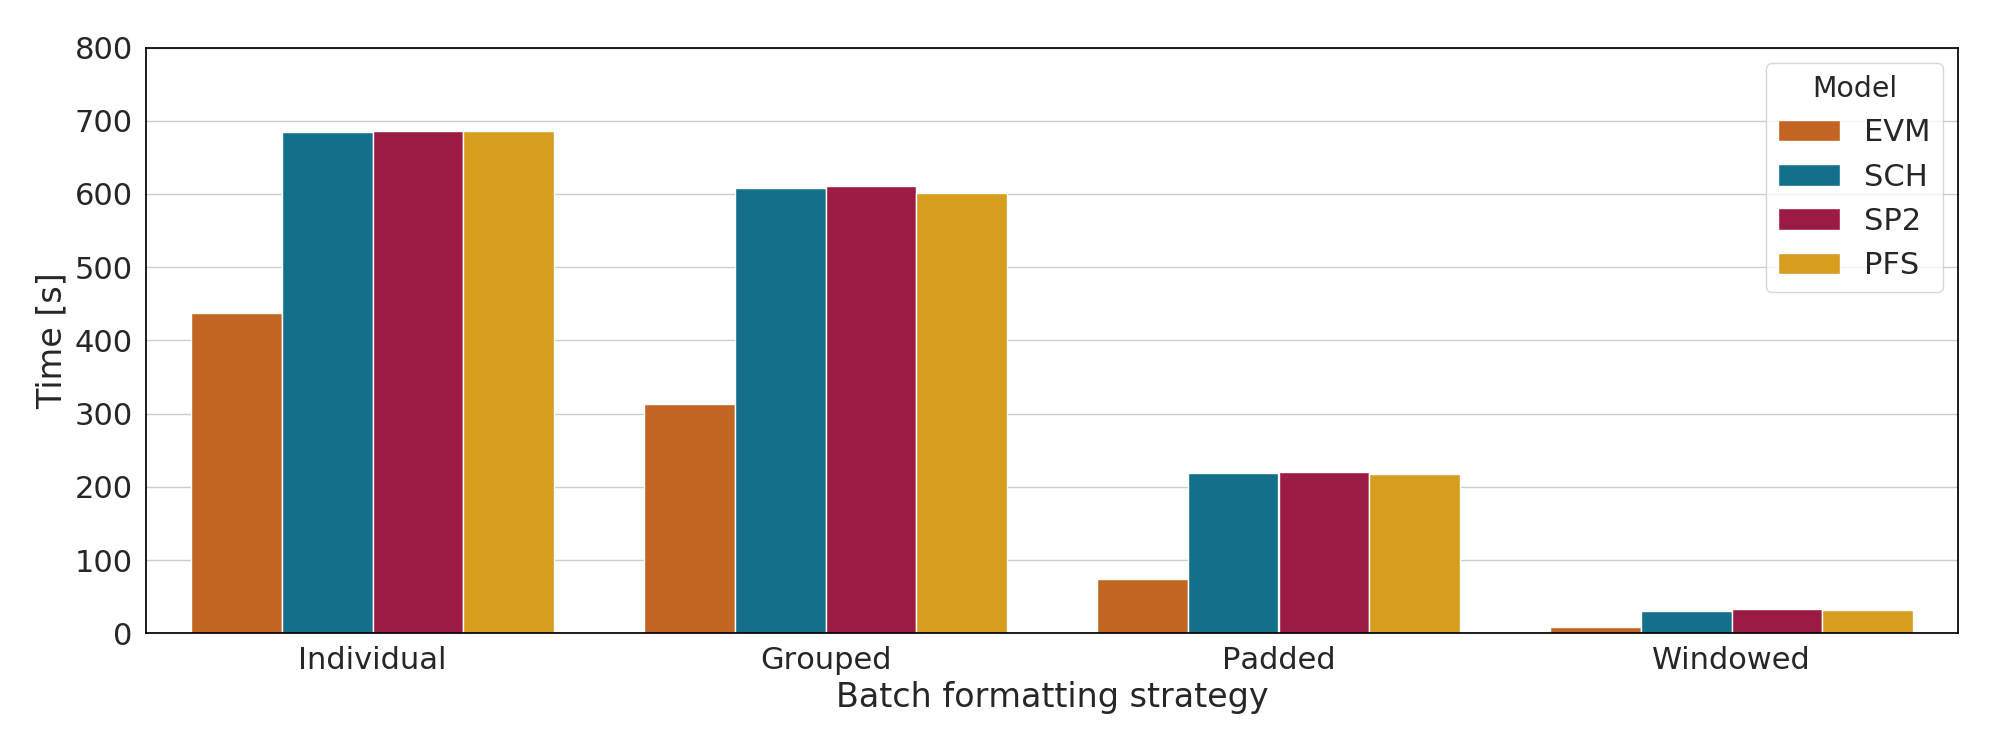
\includegraphics[width=\textwidth]{gfx/bpic2011/train_timings.png}
    \caption{Training times measured on the BPIC11~\cite{BPIC2011} dataset}
    \label{fig:BPIC11-training-timings}
\end{figure}
\begin{figure}
    \centering
    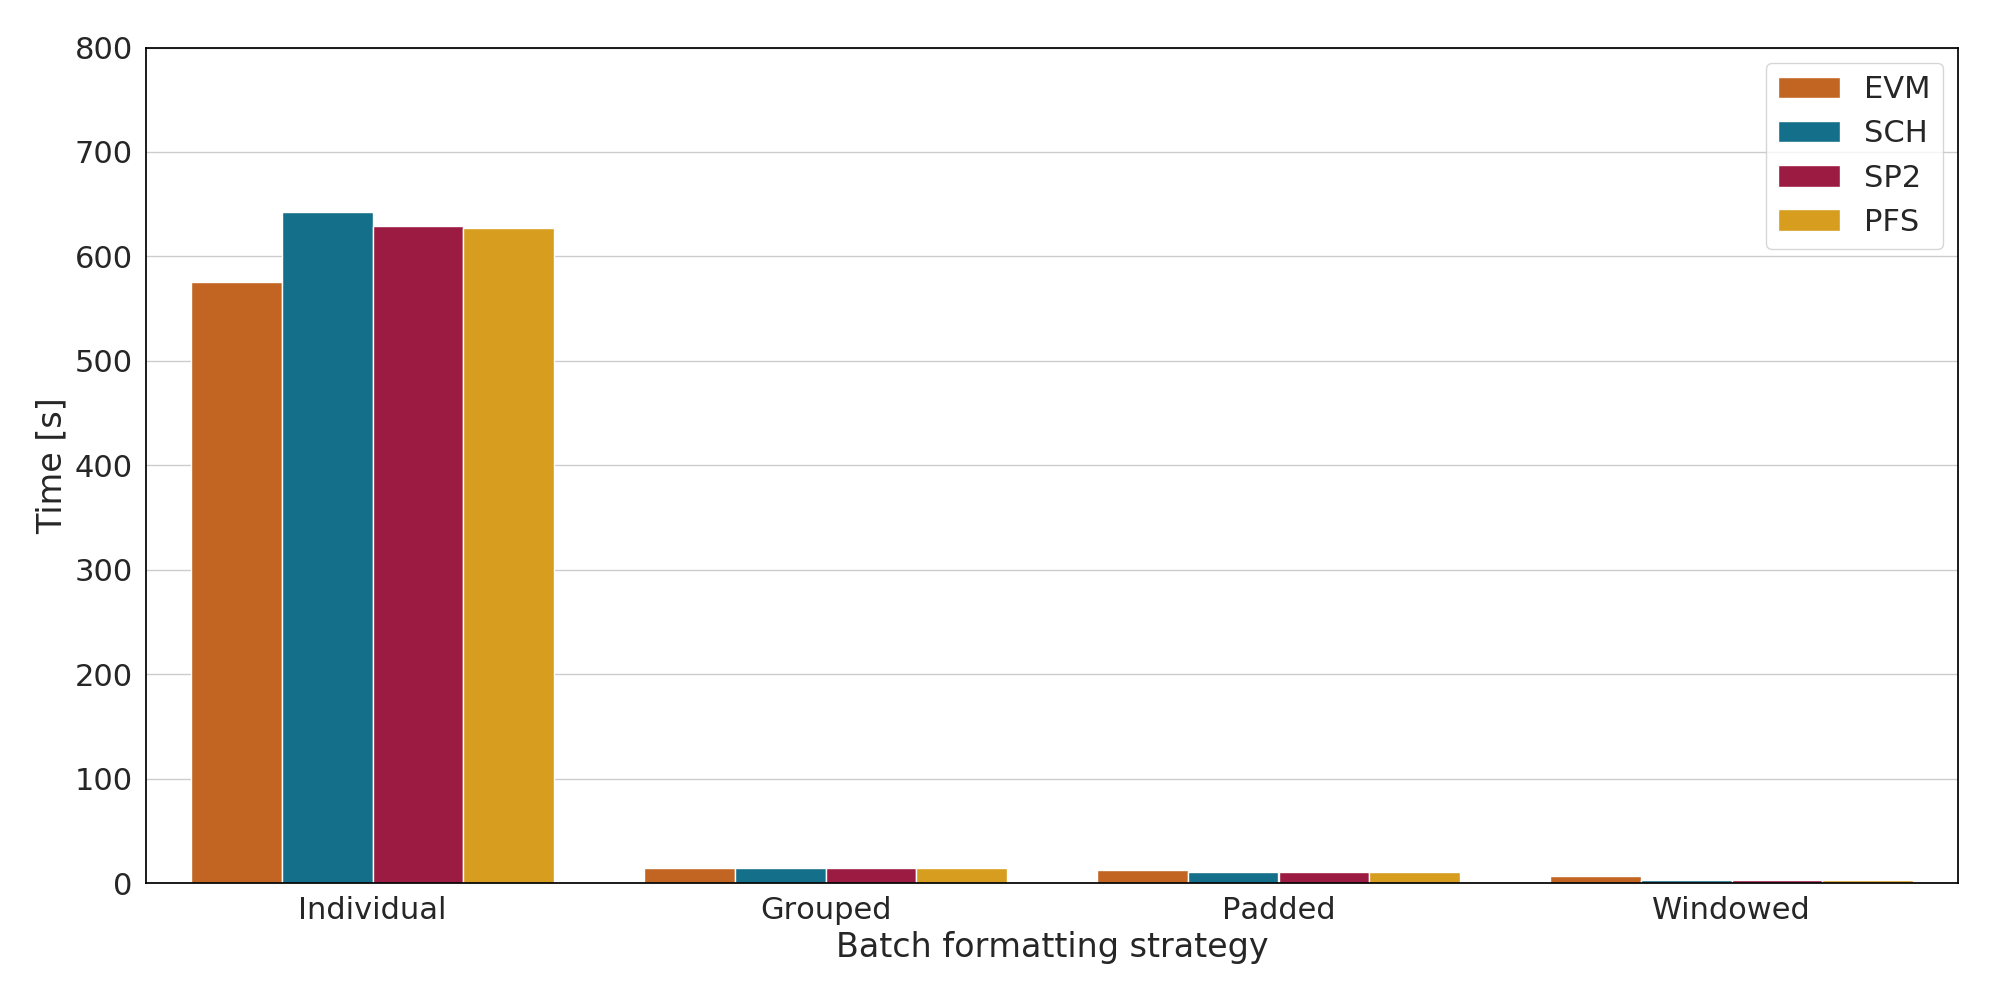
\includegraphics[width=\textwidth]{gfx/bpic2012/train_timings.png}
    \caption{Training times measured on the BPIC12~\cite{BPIC2012} dataset}
    \label{fig:BPIC12-training-timings}
\end{figure}
\begin{figure}
    \centering
    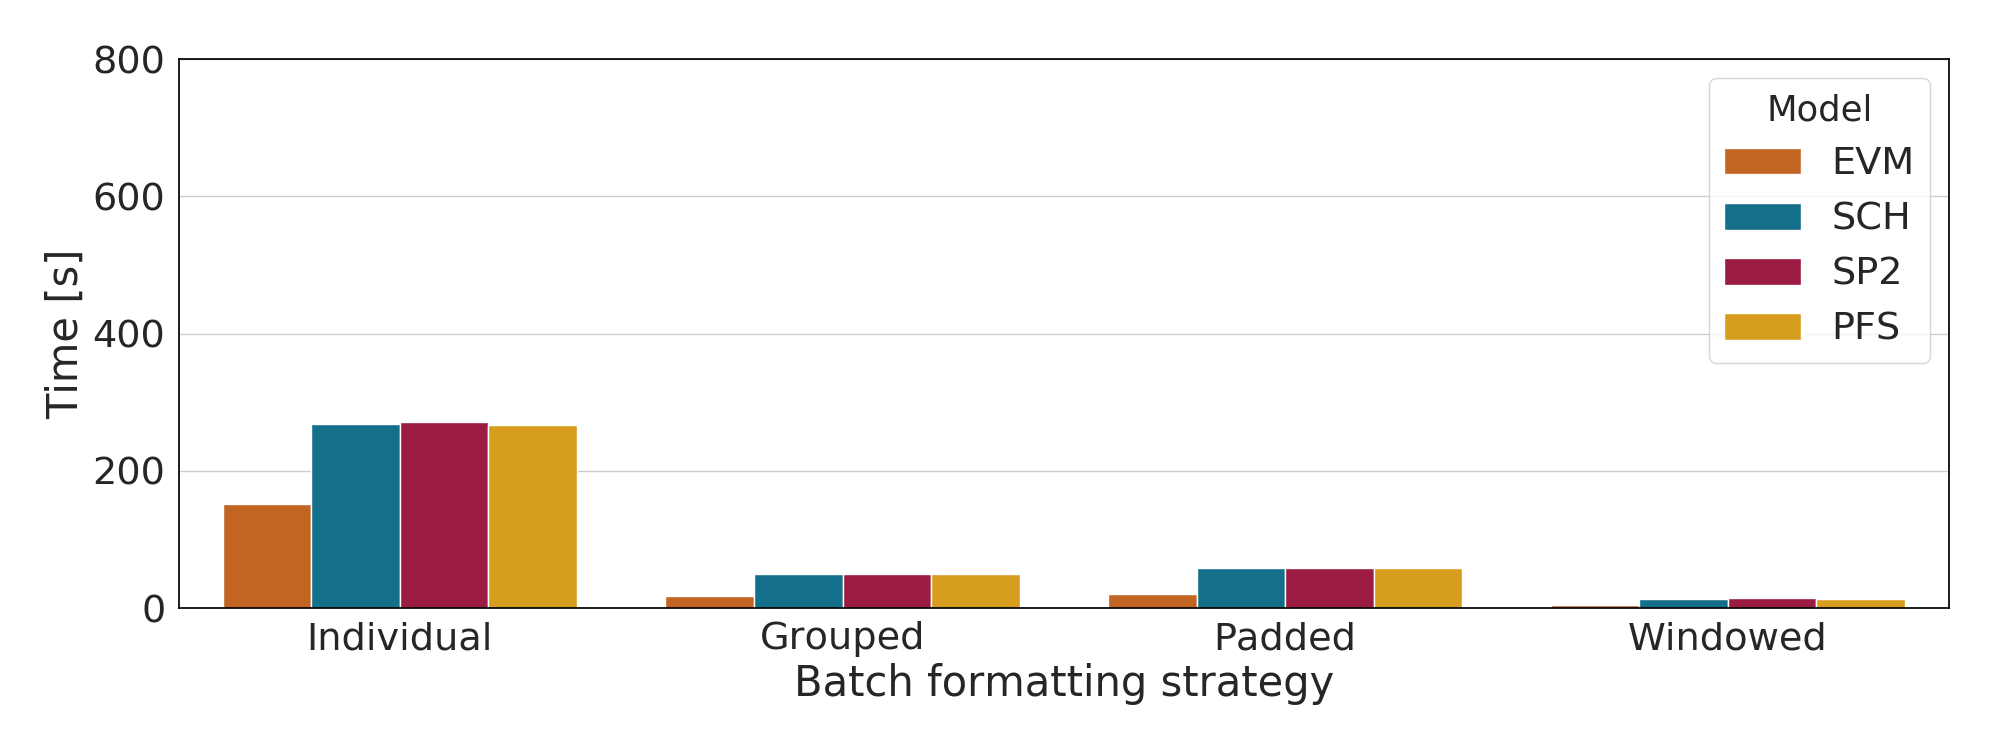
\includegraphics[width=\textwidth]{gfx/bpic2015_1/train_timings.png}
    \caption{Training times measured on the BPIC15-1~\cite{BPIC2015} dataset}
    \label{fig:BPIC15-1-training-timings}
\end{figure}
\begin{figure}
    \centering
    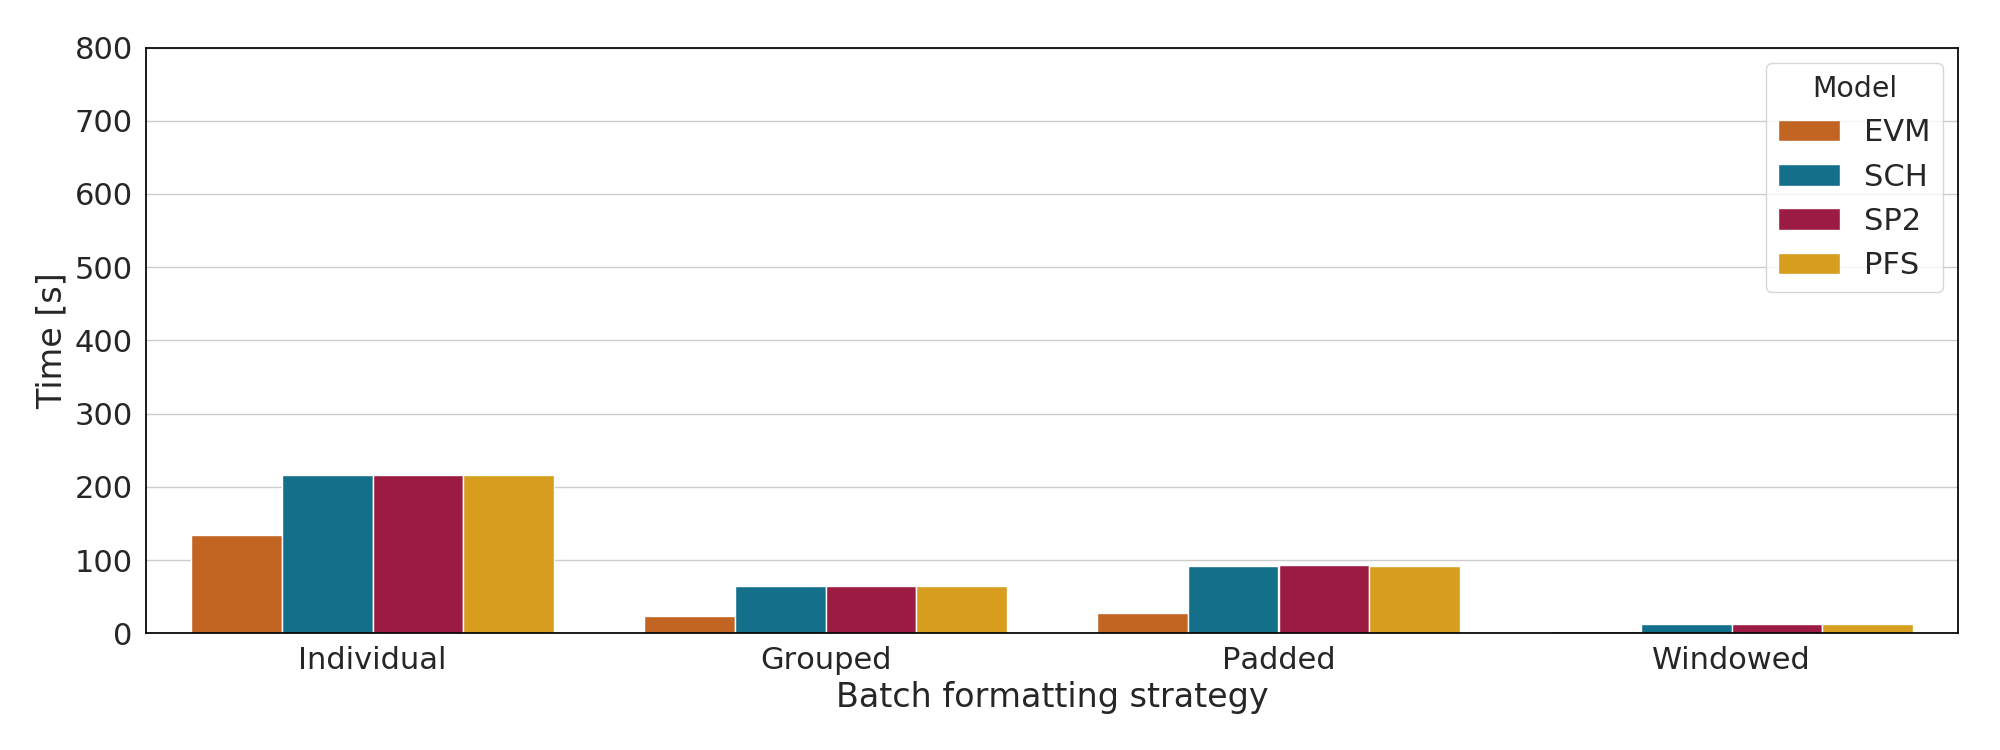
\includegraphics[width=\textwidth]{gfx/bpic2015_2/train_timings.png}
    \caption{Training times measured on the BPIC15-2~\cite{BPIC2015} dataset}
    \label{fig:BPIC15-2-training-timings}
\end{figure}
\begin{figure}
    \centering
    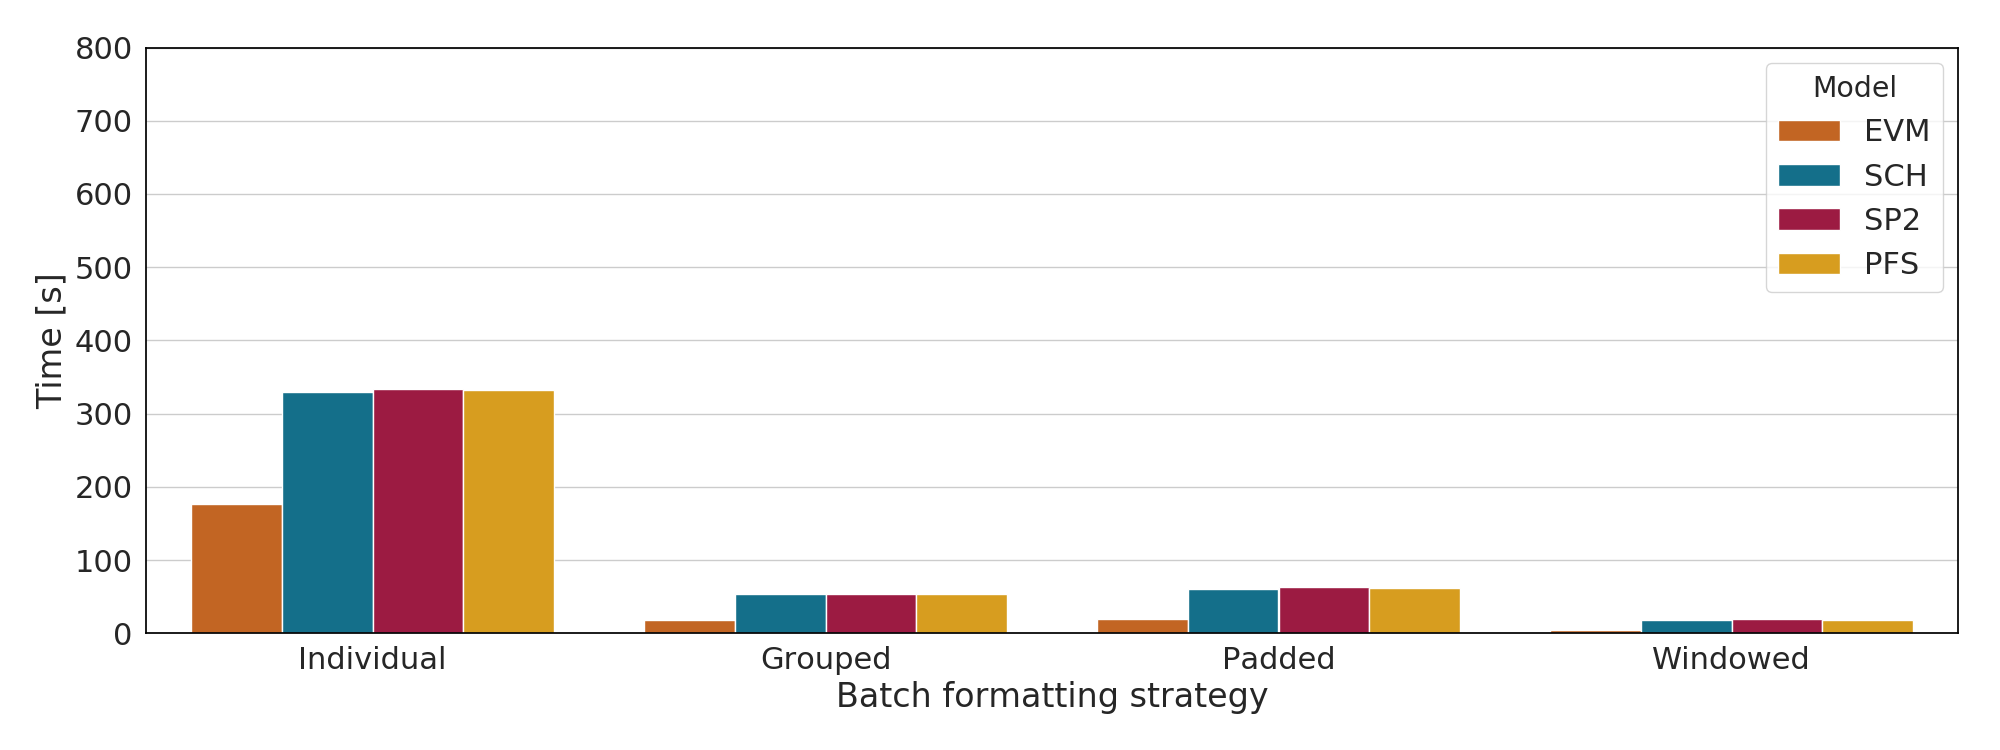
\includegraphics[width=\textwidth]{gfx/bpic2015_3/train_timings.png}
    \caption{Training times measured on the BPIC15-3~\cite{BPIC2015} dataset}
    \label{fig:BPIC15-3-training-timings}
\end{figure}
\begin{figure}
    \centering
    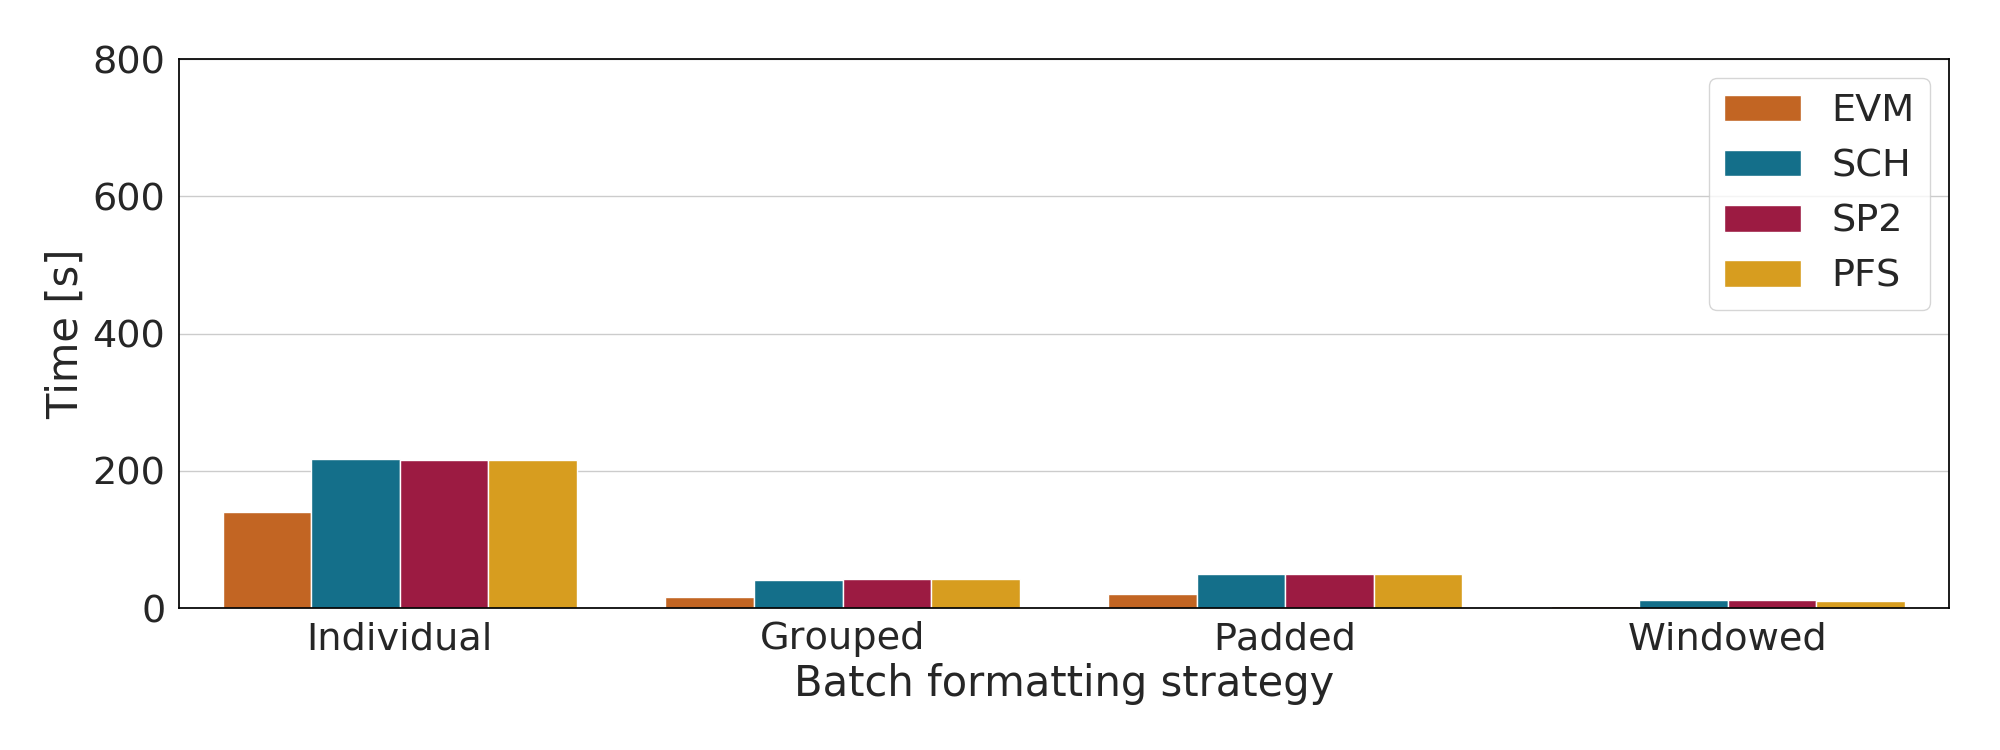
\includegraphics[width=\textwidth]{gfx/bpic2015_4/train_timings.png}
    \caption{Training times measured on the BPIC15-4~\cite{BPIC2015} dataset}
    \label{fig:BPIC15-4-training-timings}
\end{figure}
\begin{figure}
    \centering
    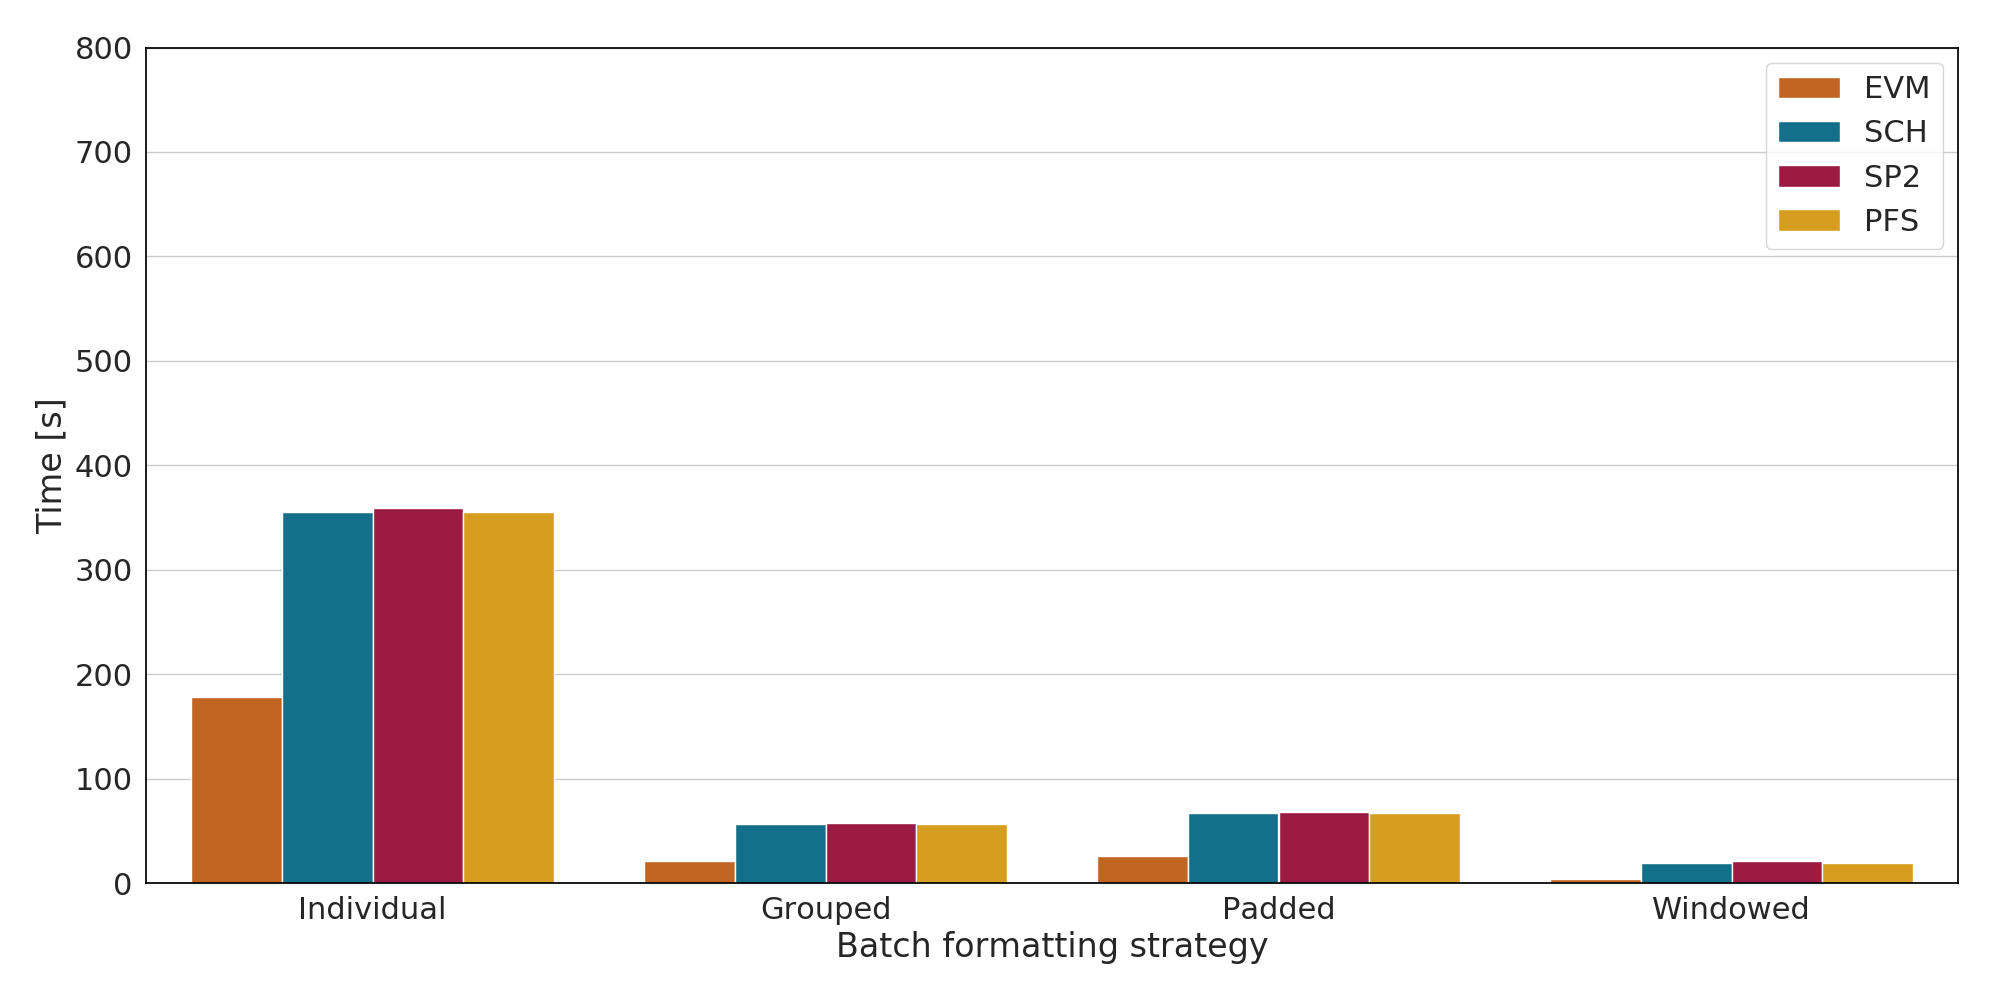
\includegraphics[width=\textwidth]{gfx/bpic2015_5/train_timings.png}
    \caption{Training times measured on the BPIC15-5~\cite{BPIC2015} dataset}
    \label{fig:BPIC15-5-training-timings}
\end{figure}

\FloatBarrier
\subsection*{Stability}
As we stressed in the introduction, the stability of a prediction model along the life of a case is important for user trust. \autoref{appendix:evaluation-measurements} contains the figures that illustrate the stability of each model and batching strategy, grouped by dataset.



\section{Discussion}\label{sec:eval:discussion}
\todo[inline]{Is this really needed? Maybe discuss directly with the results?}
\chapter{Conclusion} \label{chap:conclusion}
In order to present our conclusion, we divide this chapter into two sections.
In \autoref{sec:conclusion:verdict}, we recapitulate the results of our work.
We elaborate on our limitations and connect them to steps with which to carry research further in \autoref{sec:conclusion:future-work}.

\section{Summary of the results} \label{sec:conclusion:verdict}
In this thesis, we compared four different neural network architectures on three criteria in predicting the next activity in a running case.
The comparison was implemented in Python and Keras and yielded a neural network training framework for sequence prediction.
It allows for quickly training different network architectures with different batch construction strategies for variable-length traces.
The dataset for training can be exchanged.\\

\noindent The framework not only allows for training numerous model-strategy-dataset combinations but also tackles an issue within current research: comparability.
Most publications in Predictive Process Monitoring use different datasets and do not publicize their implementation, thus making comparisons hard.
It is considered standard practice in machine learning research to make code and datasets accessible for reproduction~\cite{russell1995modern}.
By using our framework, researchers only need to make the implementations of the base classes accessible to the public along with the data.
Because the framework covers a large part of typical training logic, development time is also reduced.\\

To establish a baseline, we implemented two of the four neural network models from publications by Evermann et al. and Schönig et al.~\cite{evermann2016, schoenig2018}.
We then ported an approach from NLP to Predictive Process Monitoring, resulting in a third model~\cite{shibata2016bipartite}.
By adapting the input features of the ported model per the findings of another publication, we obtained a fourth model~\cite{klinkmuller2018reliablemonitoring}.
In the order of introduction, we refer to the four models as EVM, SCH, SP2, and PFS.\\

In our evaluation, we focused on prediction accuracy, training time, and the stability of the prediction accuracy over time.
The SP2 model consistently ranked at the top or among the best performing models, which we attribute to the use of SP-2 features. In comparison with recently published accuracy numbers on the BPIC12 log, the SCH and SP2 models were more accurate by $0.07$ and attained $0.853$ and $0.850$~\cite{boehmer2018probability, evermann2016}.
On the HelpDesk log, the PFS and SCH models outperformed the published numbers, too, and reached accuracies of $0.862$ and $0.854$.

Furthermore, we learned that grouping traces by their length to produce batches contributes to the highest accuracies with the smallest training time.
Generally, the batching strategies which supply complete history to the model perform best.
The strategy of using a single trace per batch sees the smallest accuracy gains and requires the most time to train an epoch.

Another finding of the measurements was that process complexity seems to influence prediction accuracy.
The more activities a trace has, and the longer it tends to be, the less accurate the predictions become.
This connection was also visible in the stability measurements when process complexity went up or down in a stage of the process.

Finally, we could confirm findings from Klinkmüller et al. that omitting history from process traces negatively impacts prediction accuracy~\cite{klinkmuller2018reliablemonitoring}.

\section{Future work and limitations}\label{sec:conclusion:future-work}
In this section, we present items which could carry this research further in publications or subsequent master thesis.
We cluster the future work by topic and connect our limitations where applicable.

\paragraph{Benchmarking dataset} Currently, Predictive Process Monitoring suffers from not having standardized benchmarking datasets for researchers to evaluate their algorithms on.
This forces researchers to resort to a multitude of datasets, or to even use non-public data.
In our case, we used the BPIC12 and HelpDesk logs for evaluation and accuracy comparison.
We feel that the HelpDesk log with its two columns can neither be considered a realistic nor an optimal source of data for this use case.
This is why we advocate for standard benchmarking datasets, which are common in many other machine learning disciplines.
We believe that it is time to draw up such datasets with real data or close to real-world data, representing industry-typical processes.
By having different datasets with different characteristics, prediction approaches could be evaluated along different dimensions.
As there is already a tendency to use BPIC logs, the next year's challenge could be on Predictive Process Monitoring.
There, a log could be advertised as a future standard to evaluate on.
Otherwise, the number of datasets that researchers have to use to ensure comparability will only ever increase.

\paragraph{Imbalanced classes} Predictive models learn better with a balanced target class distribution.
The prediction targets, activities in our case, are not distributed uniformly across traces.
This distribution problem is also commonly encountered in NLP.
Weighting classes based on their occurrence is a possibility to deal with it.
Keras offers a mechanism to set the weights on a per-batch basis, which could see accuracy gains~\cite{web:stackoverflow-keras-class-weights}.
We did not pursue this possibility, as our goal was to evaluate different types of models and batching strategies, and not to maximize the performance of a single model.

\paragraph{Feature engineering and hyper-parameter tuning} The PFS model uses a binary feature vector.
Every bit inside it encodes the occurrence of a single subsequence.
We chose that the vector should encode the presence of the 25 closed subsequences with the highest support of the respective dataset.
We chose not to optimize the number of encoded subsequences, as our goal was different from maximizing accuracy gains from feature engineering.
However, the chosen threshold should be varied and explored further, as it most likely differs for each dataset.
It could also be made relative to a minimum support value so that the PFS feature vector covers a different number of features for each dataset.
Furthermore, none of the model's hyper-parameters, e.g., hidden layer dimensions or activation functions, were optimized.
This would incur further gains in accuracy.

\paragraph{Data augmentation} Image data for machine learning applications is often augmented to increase the number of available training samples.
In this case, images are rotated, transformed, stretched or cropped and saved as separate samples~\cite{Thoma:2017,}.
More data generally leads to higher accuracies and more robust models.
In the interest of improving model performance for Predictive Process Monitoring, augmentation methods should be explored with which to produce more traces from existing logs.

\paragraph{Listing of best event attributes} The predictive power that a feature possesses can be measured with different methods.
If, e.g., a feature by itself exactly indicates what the next activity is going to be, its predictive power is very high.
During the analysis of a log for prediction, it is essential to isolate features with high predictive power and discard those with low predictive power.
Most event logs are saved in the XES format, which guarantees the type of information that is stored in an attribute.
In the interest of speeding up feature selection in the future, we believe that it is worthwhile to investigate the predictive power across XES standard attributes for a large number of logs.
From the findings, a list could be made of those attributes which are most likely to possess high predictive power and incur accuracy gains.

\paragraph{Word embeddings} Word embeddings for NLP applications are trained on huge text corpora like Wikipedia and help map dictionary-encoded words to a large feature space.
In \autoref{sec:background:feature-engineering}, we hinted at the fact that the weights for word embeddings can be imported from pre-trained models to avoid training on a similarly large dataset and save time.
This principle could be transferred to Predictive Process Monitoring by providing pre-trained embeddings for process categories.
As evidenced in \autoref{sec:eval:discussion}, this is tied to larger datasets.
It is worth exploring how well activity names are similar across processes, to gauge the reusability of a word embedding produced on one process for another.

\paragraph{Process optimization} We have seen that the accuracy of a model can be influenced by the variability of the process in a specific stage.
For stages in a process where there are not many activities or any decisions, prediction accuracy tends to be high.
Assuming that all data on which decisions are usually based are provided to the model, we believe that accuracy drops can indicate optimization potential in the process.
If the model can not understand the connections in the data, it could mean that the control flow decisions are overly complicated or do not follow a standard.
Whether this is the case, and what process fallacies can be detected based on accuracy fluctuation should be investigated.


%\cleardoublepage % Empty page before the start of the next part

%----------------------------------------------------------------------------------------
%	THESIS CONTENT - APPENDICES
%----------------------------------------------------------------------------------------

\appendix
\part*{Appendix}
\renewcommand{\thefigure}{A.\arabic{figure}}
\chapter{Correlation heatmaps}
\begin{figure}[ht!]
\centering
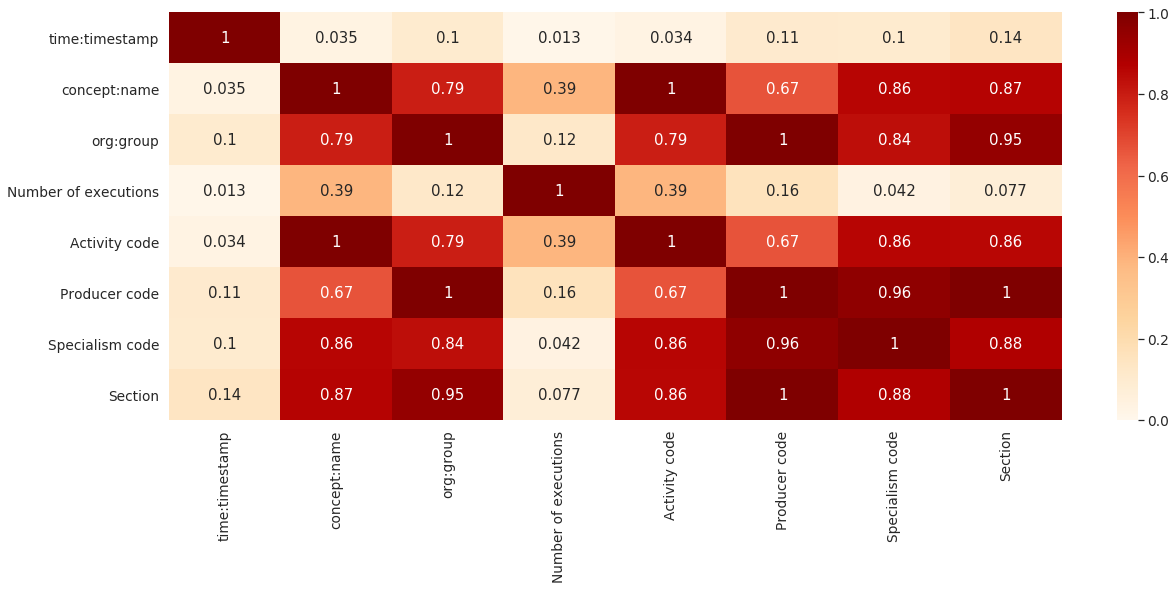
\includegraphics[width=\textwidth]{gfx/bpic11-correlation-heatmap.png}
\caption{Heatmap of correlating values within the BPIC11 dataset, obtained using pair-wise application of Cramér's~V}
\label{fig:BPIC11-correlation-heatmap}
\end{figure}

\begin{figure}[ht!]
\centering
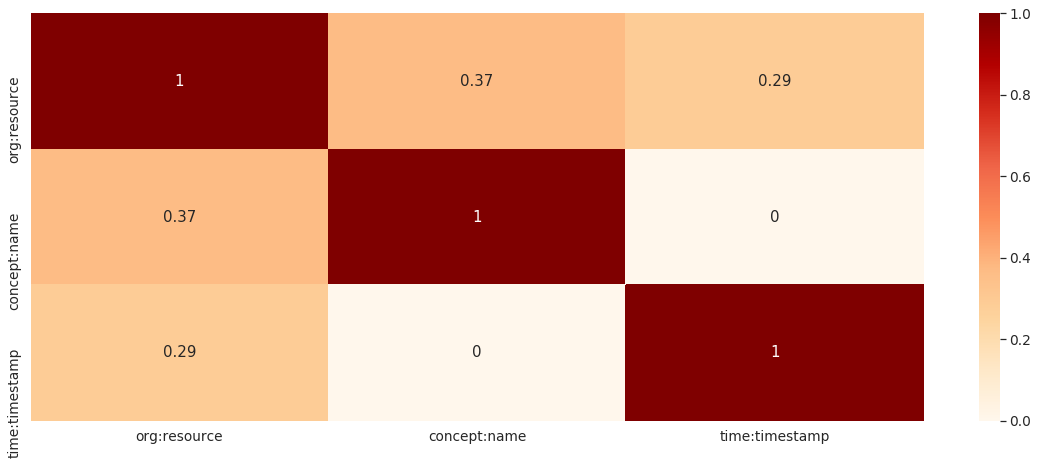
\includegraphics[width=\textwidth]{gfx/bpic12-correlation-heatmap.png}
\caption{Heatmap of correlating values within the BPIC12 dataset, obtained using pair-wise application of Cramér's~V}
\label{fig:BPIC12-correlation-heatmap}
\end{figure}

\begin{figure}[ht!]
\centering
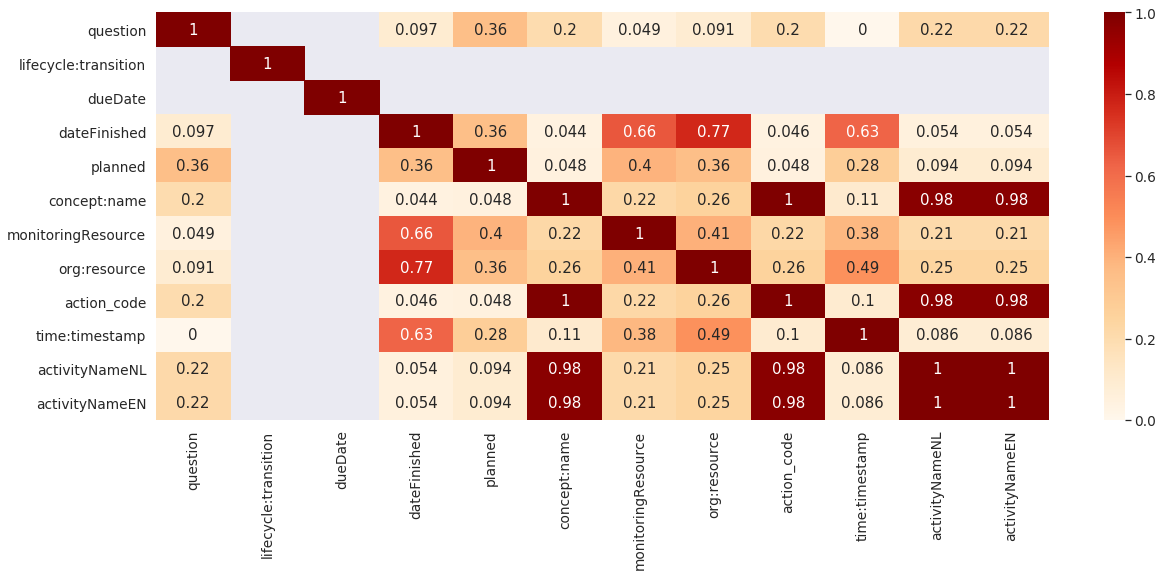
\includegraphics[width=\textwidth]{gfx/bpic15-1-correlation-heatmap.png}
\caption{Heatmap of correlating values within the BPIC15-1 dataset, obtained using pair-wise application of Cramér's~V}
\label{fig:BPIC15-1-correlation-heatmap}
\end{figure}

\begin{figure}[ht!]
\centering
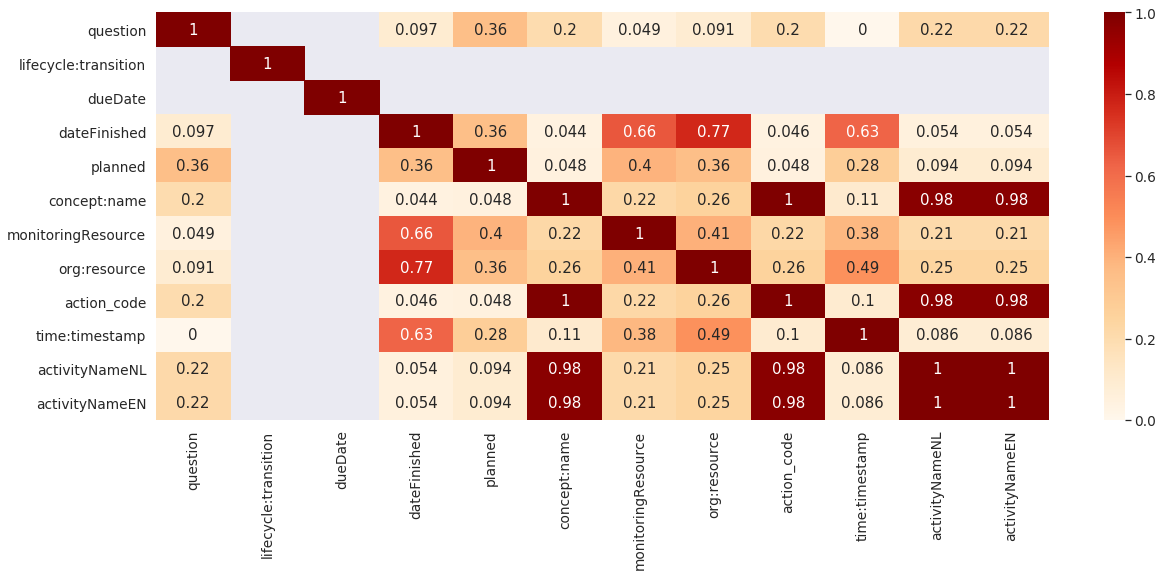
\includegraphics[width=\textwidth]{gfx/bpic15-1-correlation-heatmap.png}
\caption{Heatmap of correlating values within the BPIC15-2 dataset, obtained using pair-wise application of Cramér's~V}
\label{fig:BPIC15-2-correlation-heatmap}
\end{figure}

\begin{figure}[ht!]
\centering
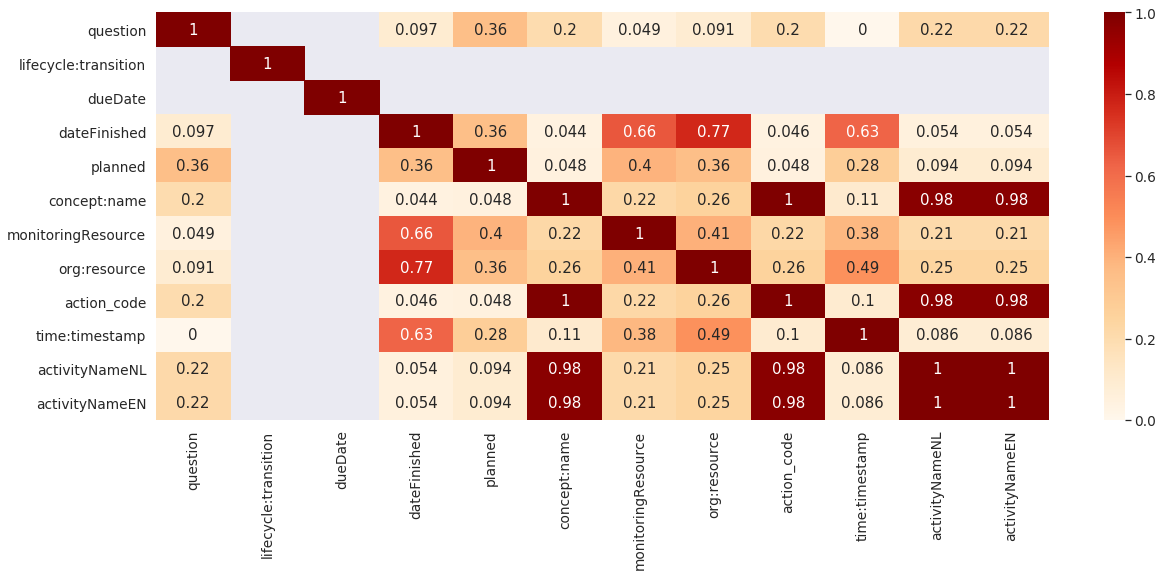
\includegraphics[width=\textwidth]{gfx/bpic15-1-correlation-heatmap.png}
\caption{Heatmap of correlating values within the BPIC15-3 dataset, obtained using pair-wise application of Cramér's~V}
\label{fig:BPIC15-3-correlation-heatmap}
\end{figure}

\begin{figure}[ht!]
\centering
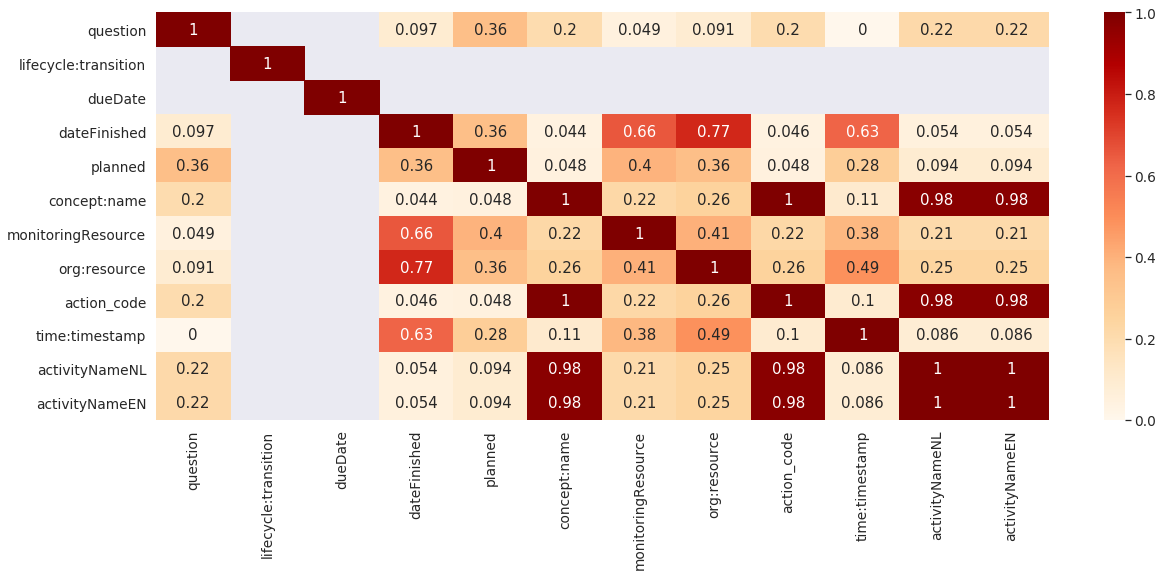
\includegraphics[width=\textwidth]{gfx/bpic15-1-correlation-heatmap.png}
\caption{Heatmap of correlating values within the BPIC15-4 dataset, obtained using pair-wise application of Cramér's~V}
\label{fig:BPIC15-4-correlation-heatmap}
\end{figure}

\begin{figure}[ht!]
\centering
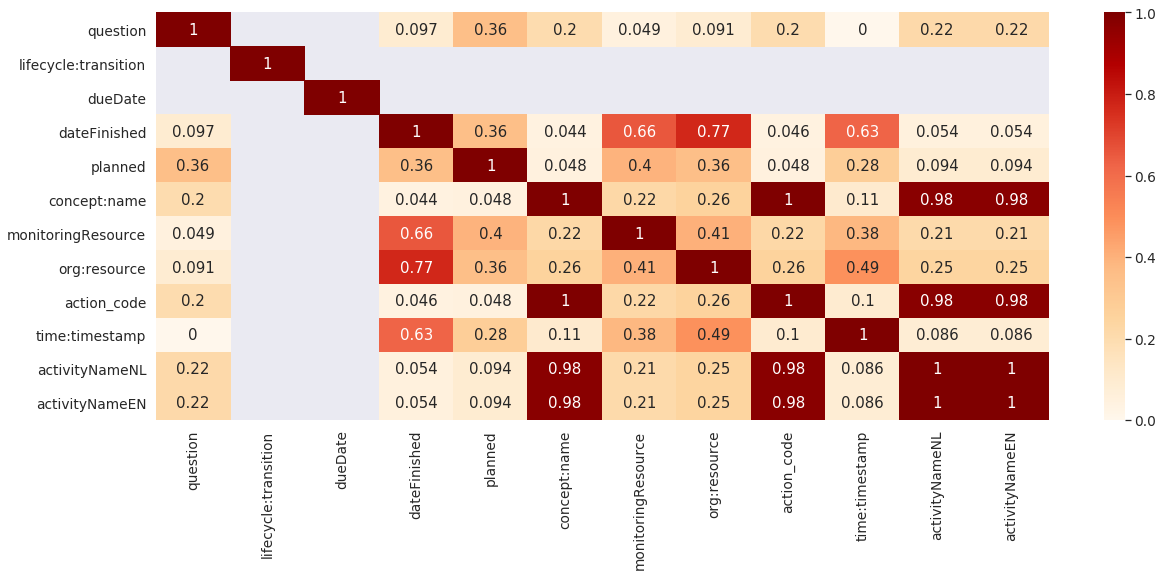
\includegraphics[width=\textwidth]{gfx/bpic15-1-correlation-heatmap.png}
\caption{Heatmap of correlating values within the BPIC15-5 dataset, obtained using pair-wise application of Cramér's~V}
\label{fig:BPIC15-5-correlation-heatmap}
\end{figure}
\renewcommand{\thefigure}{B.\arabic{figure}}
\chapter{Prediction stability}
\label{appendix:evaluation-measurements}
\section*{BPIC11}
\begin{figure}[!htb]
    \centering
    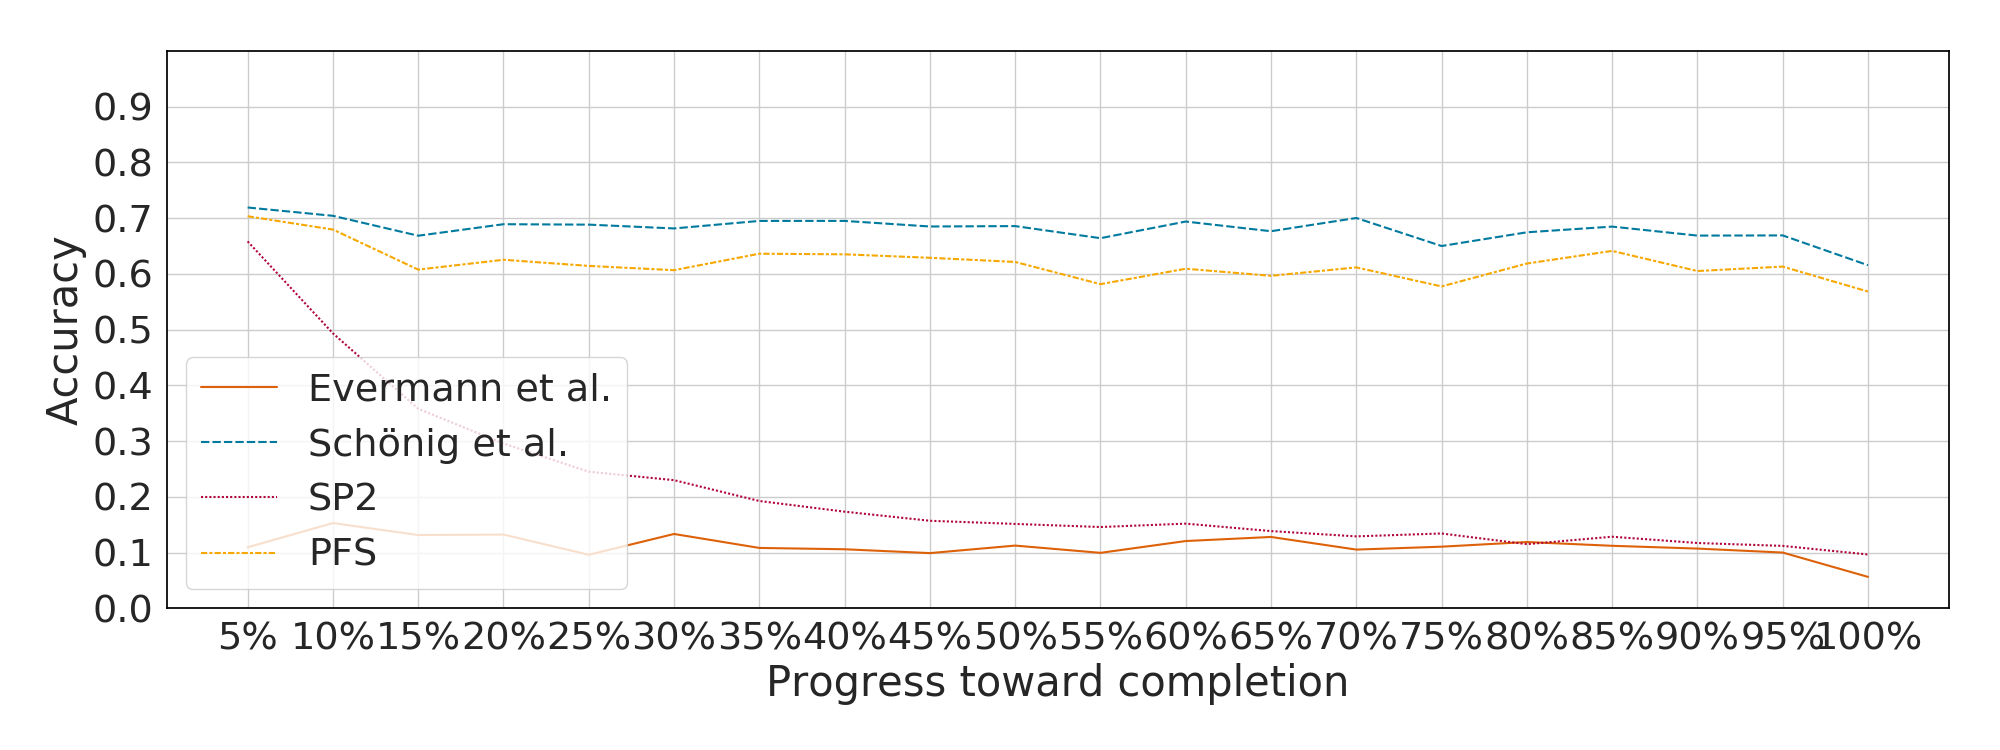
\includegraphics[width=\textwidth]{gfx/bpic2011/individual_stability.png}
    \caption{Stability of the models with the individual batching strategy on BPIC11}
    \label{fig:bpic11-individual-stability}
\end{figure}
\begin{figure}[!htb]
    \centering
    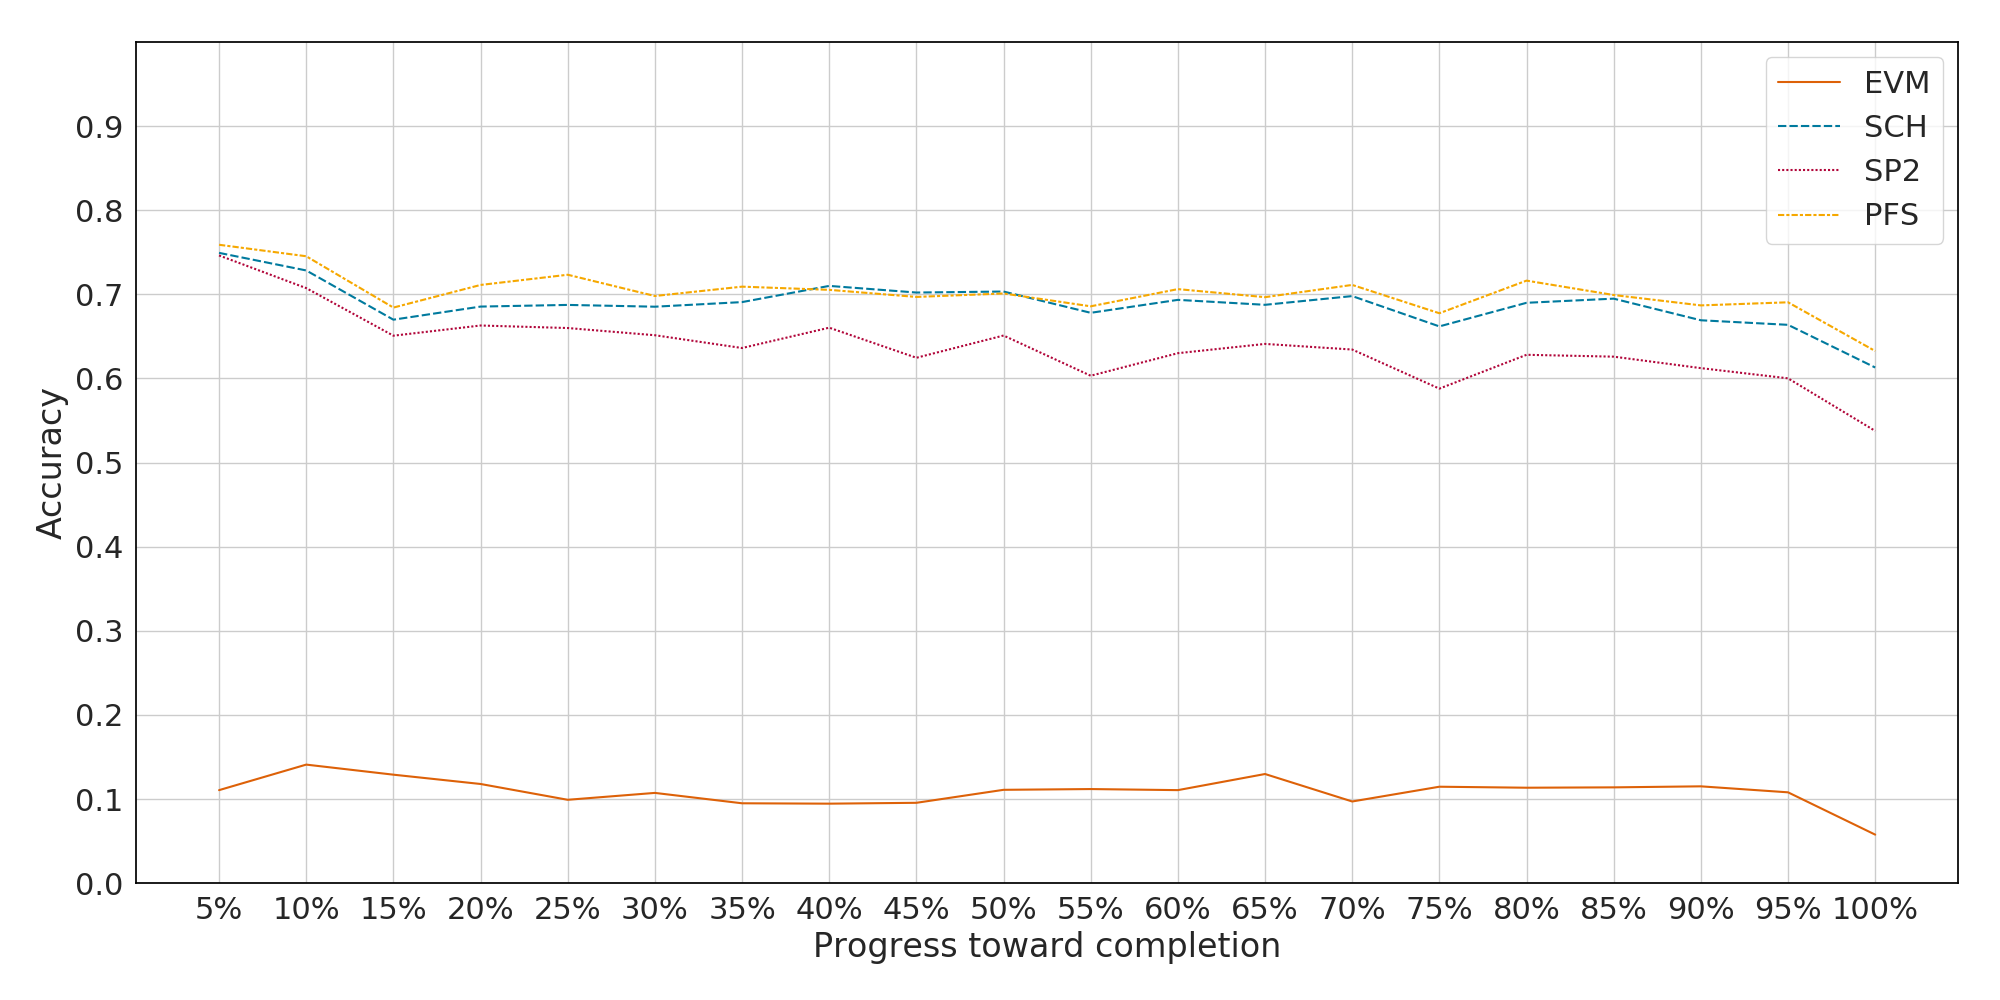
\includegraphics[width=\textwidth]{gfx/bpic2011/grouped_stability.png}
    \caption{Stability of the models with the grouped batching strategy on BPIC11}
    \label{fig:bpic11-grouped-stability}
\end{figure}
\begin{figure}[!htb]
    \centering
    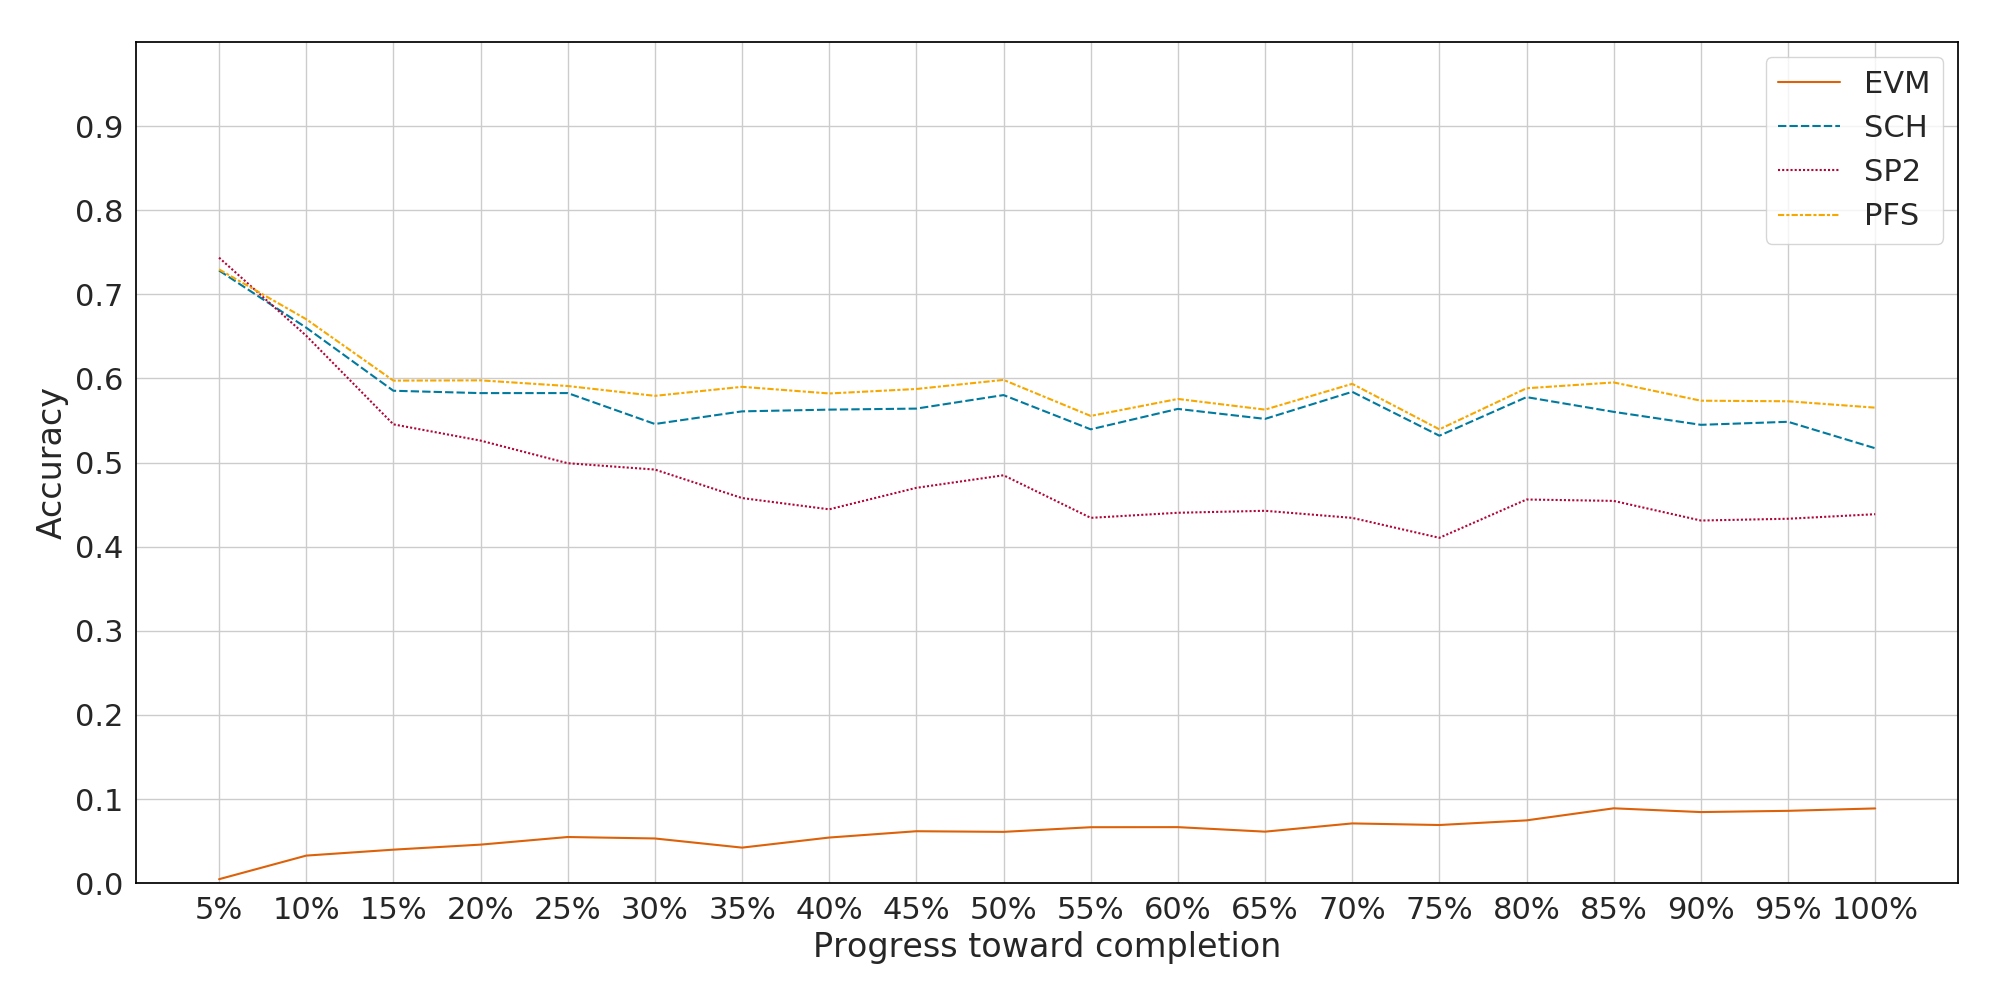
\includegraphics[width=\textwidth]{gfx/bpic2011/padded_stability.png}
    \caption{Stability of the models with the padded batching strategy on BPIC11}
    \label{fig:bpic11-padded-stability}
\end{figure}
\begin{figure}[!htb]
    \centering
    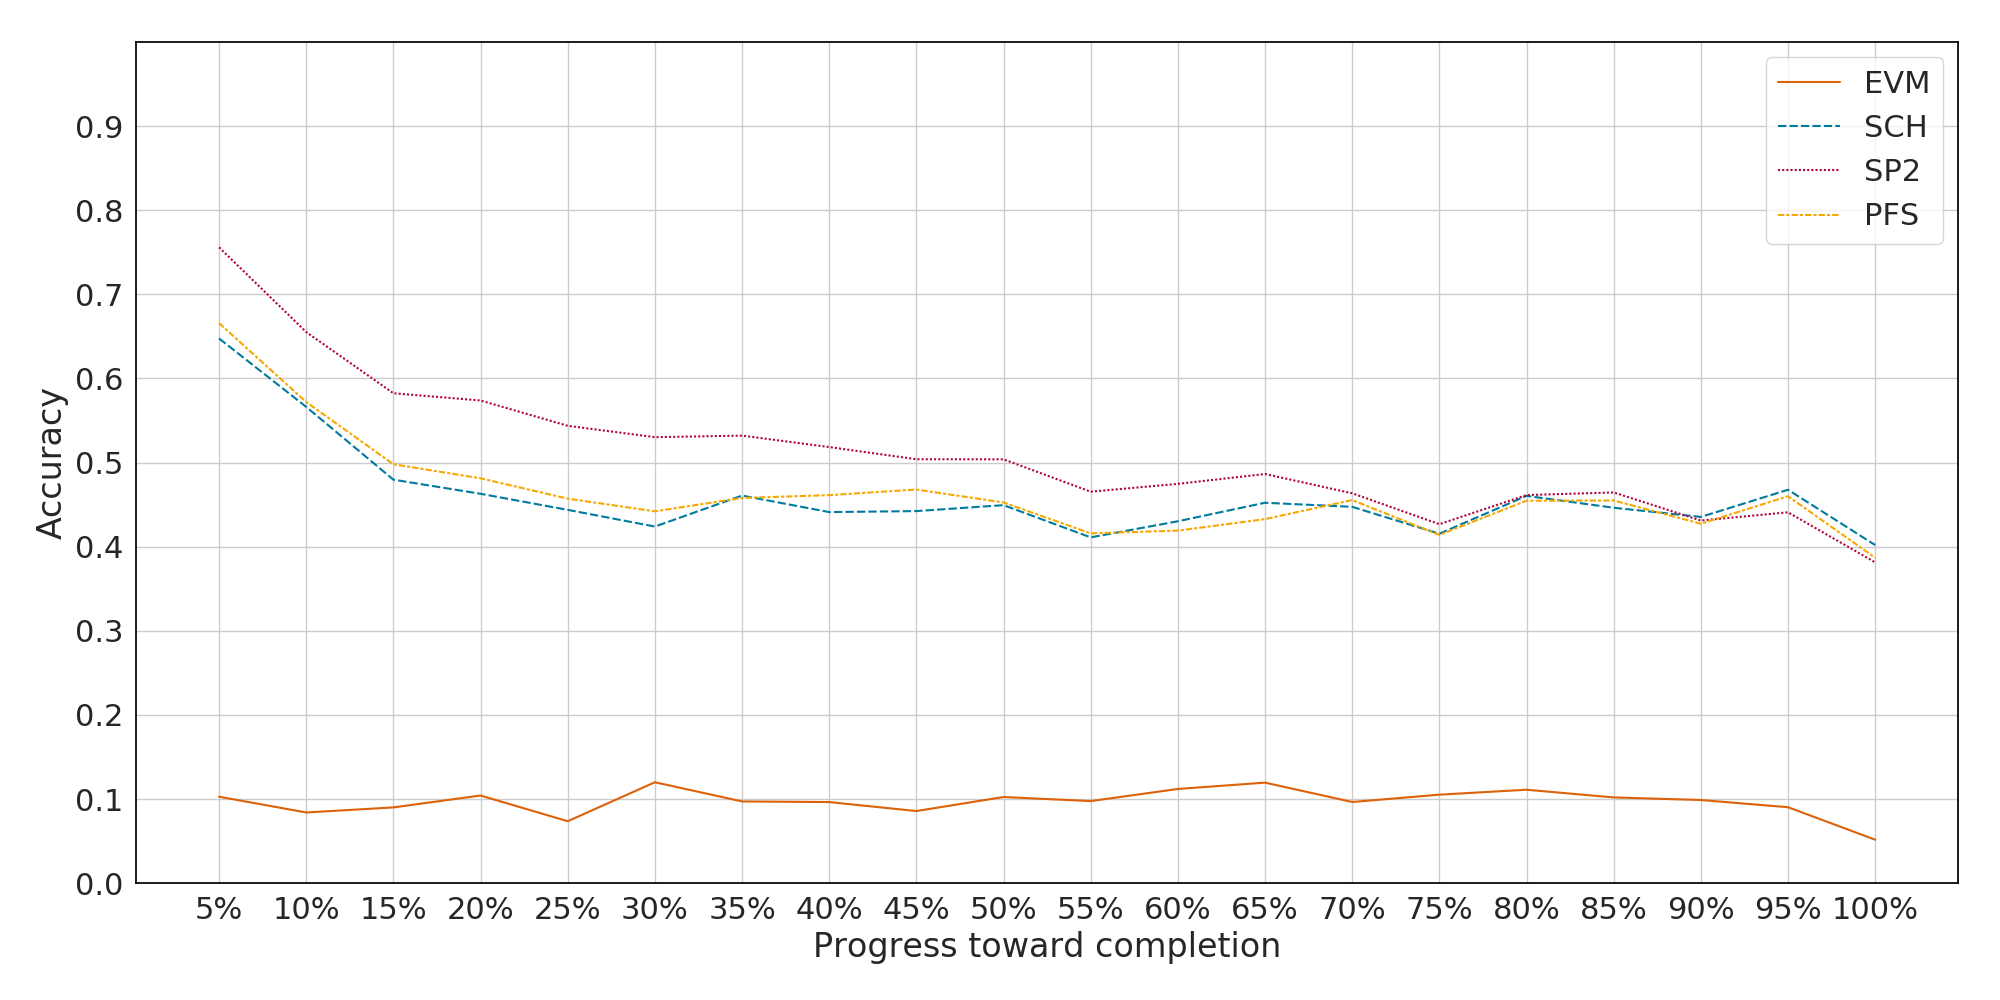
\includegraphics[width=\textwidth]{gfx/bpic2011/windowed_stability.png}
    \caption{Stability of the models with the windowed batching strategy on BPIC11}
    \label{fig:bpic11-windowed-stability}
\end{figure}
\FloatBarrier

\section*{BPIC12}
\begin{figure}[!htb]
    \centering
    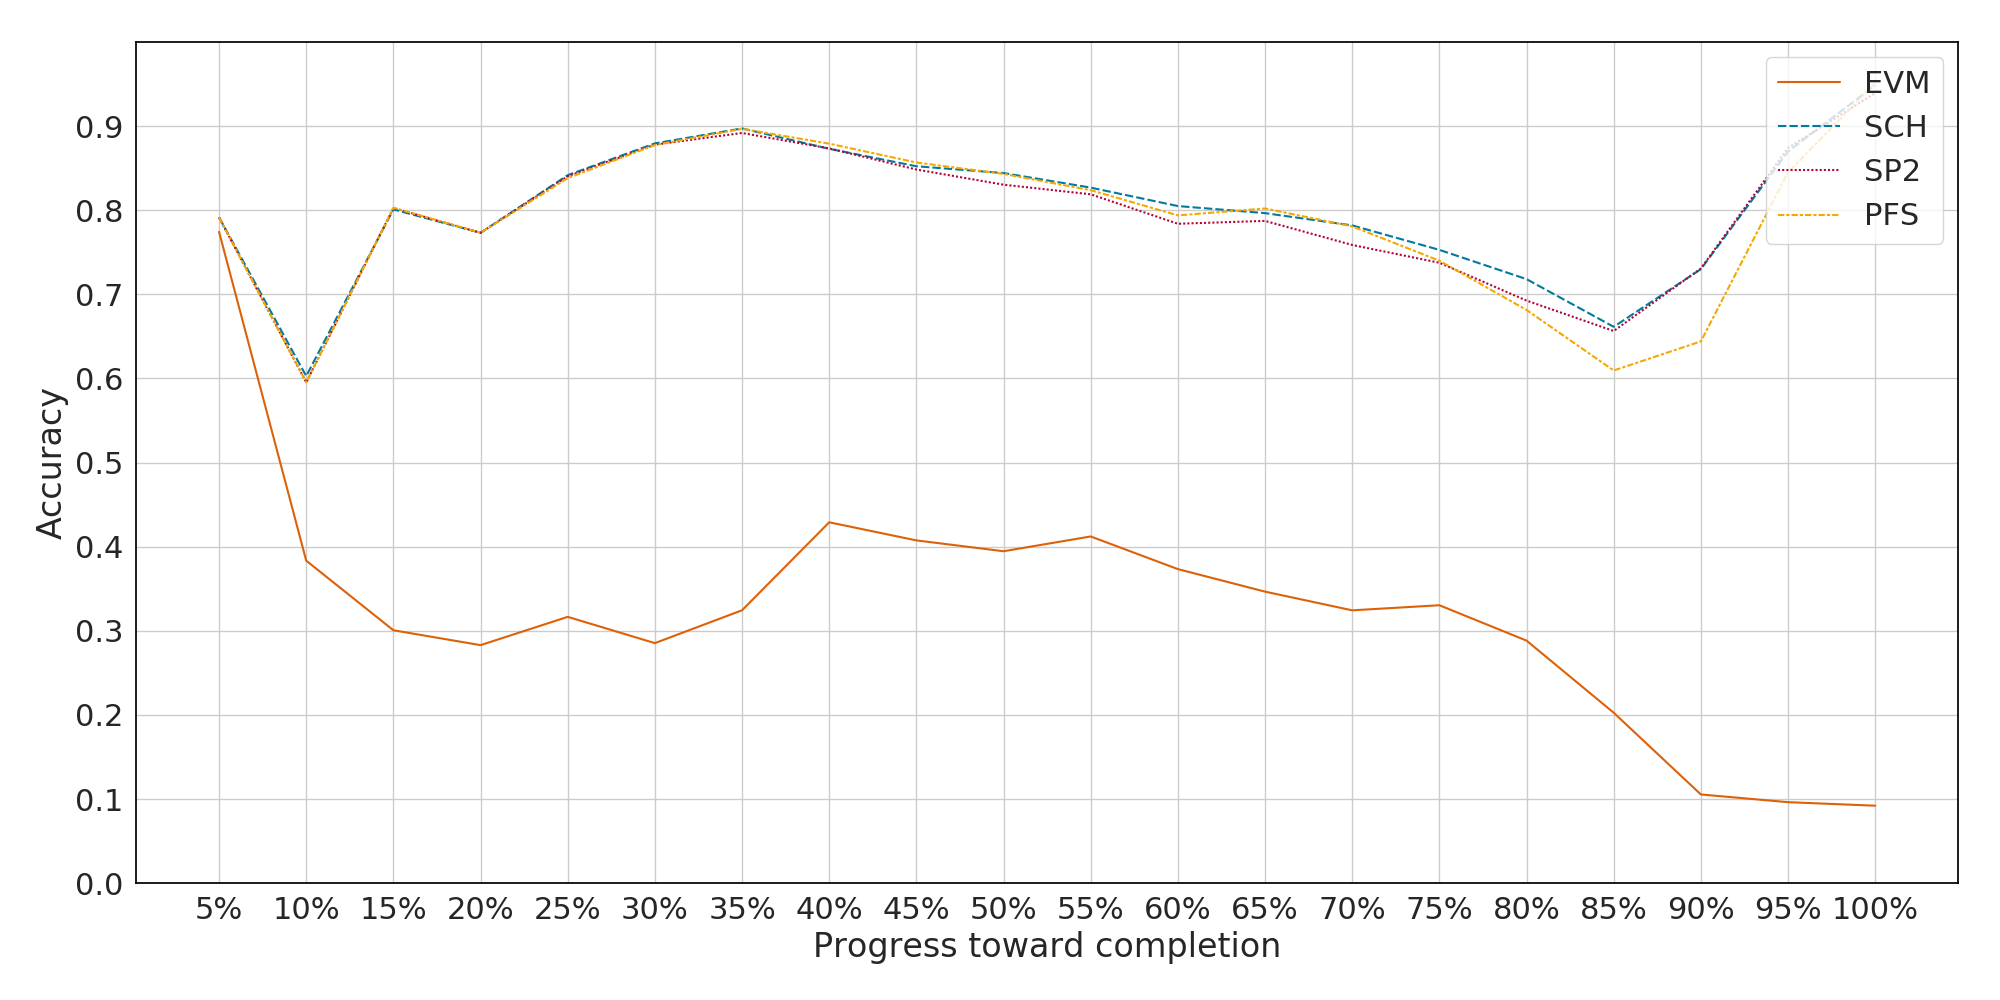
\includegraphics[width=\textwidth]{gfx/bpic2012/individual_stability.png}
    \caption{Stability of the models with the individual batching strategy on BPIC12}
    \label{fig:bpic12-individual-stability}
\end{figure}
\begin{figure}[!htb]
    \centering
    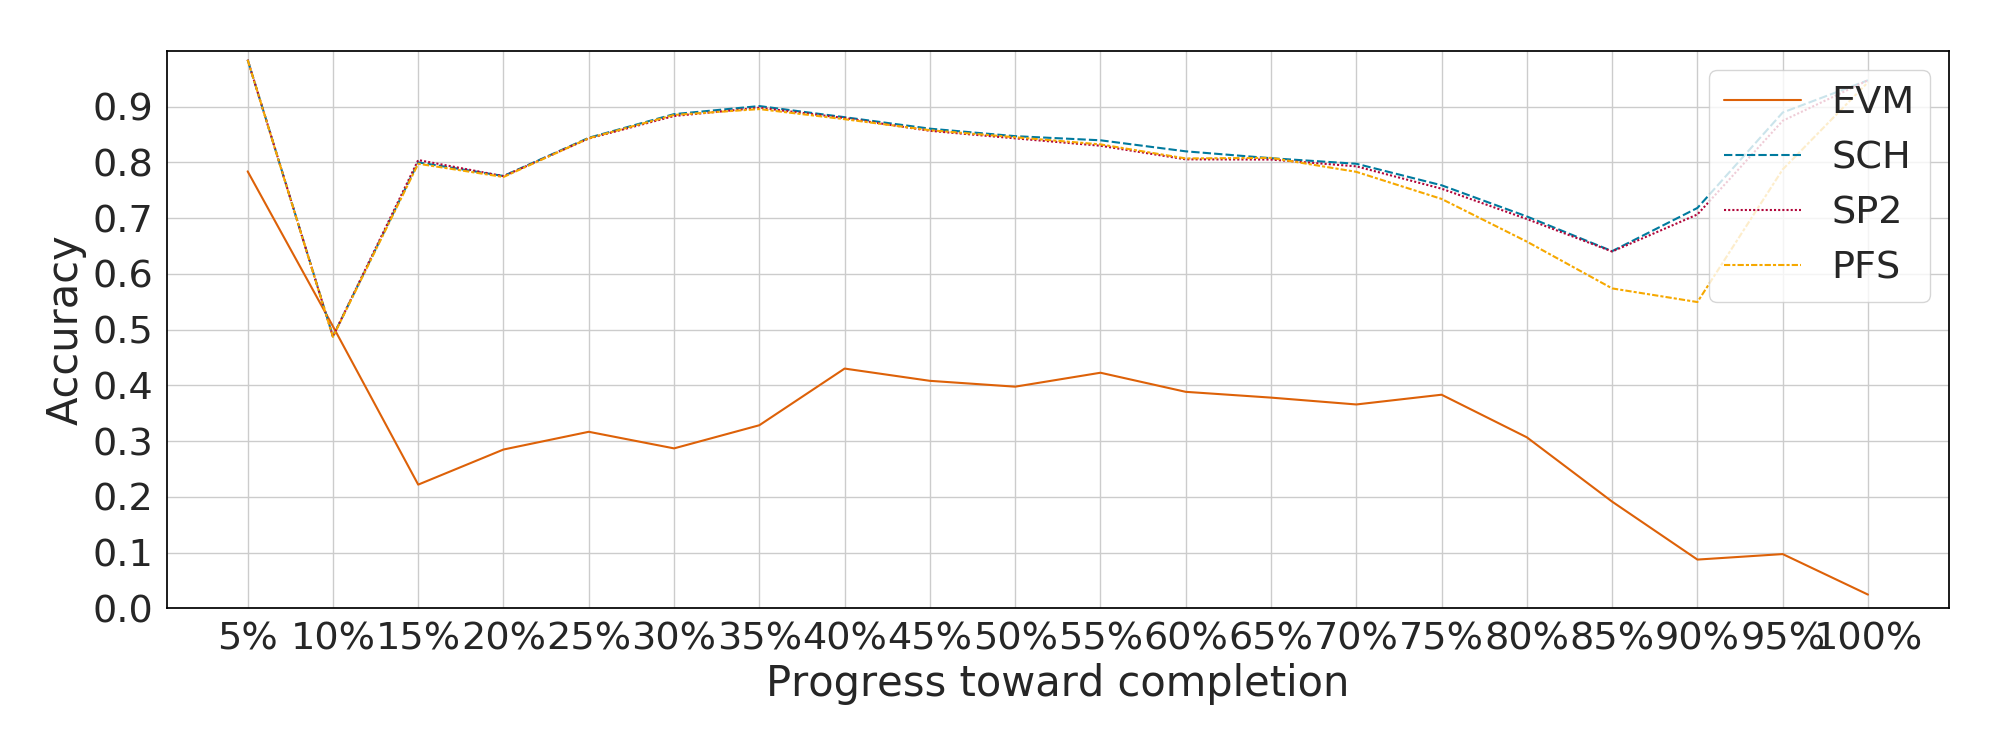
\includegraphics[width=\textwidth]{gfx/bpic2012/grouped_stability.png}
    \caption{Stability of the models with the grouped batching strategy on BPIC12}
    \label{fig:bpic12-grouped-stability}
\end{figure}
\begin{figure}[!htb]
    \centering
    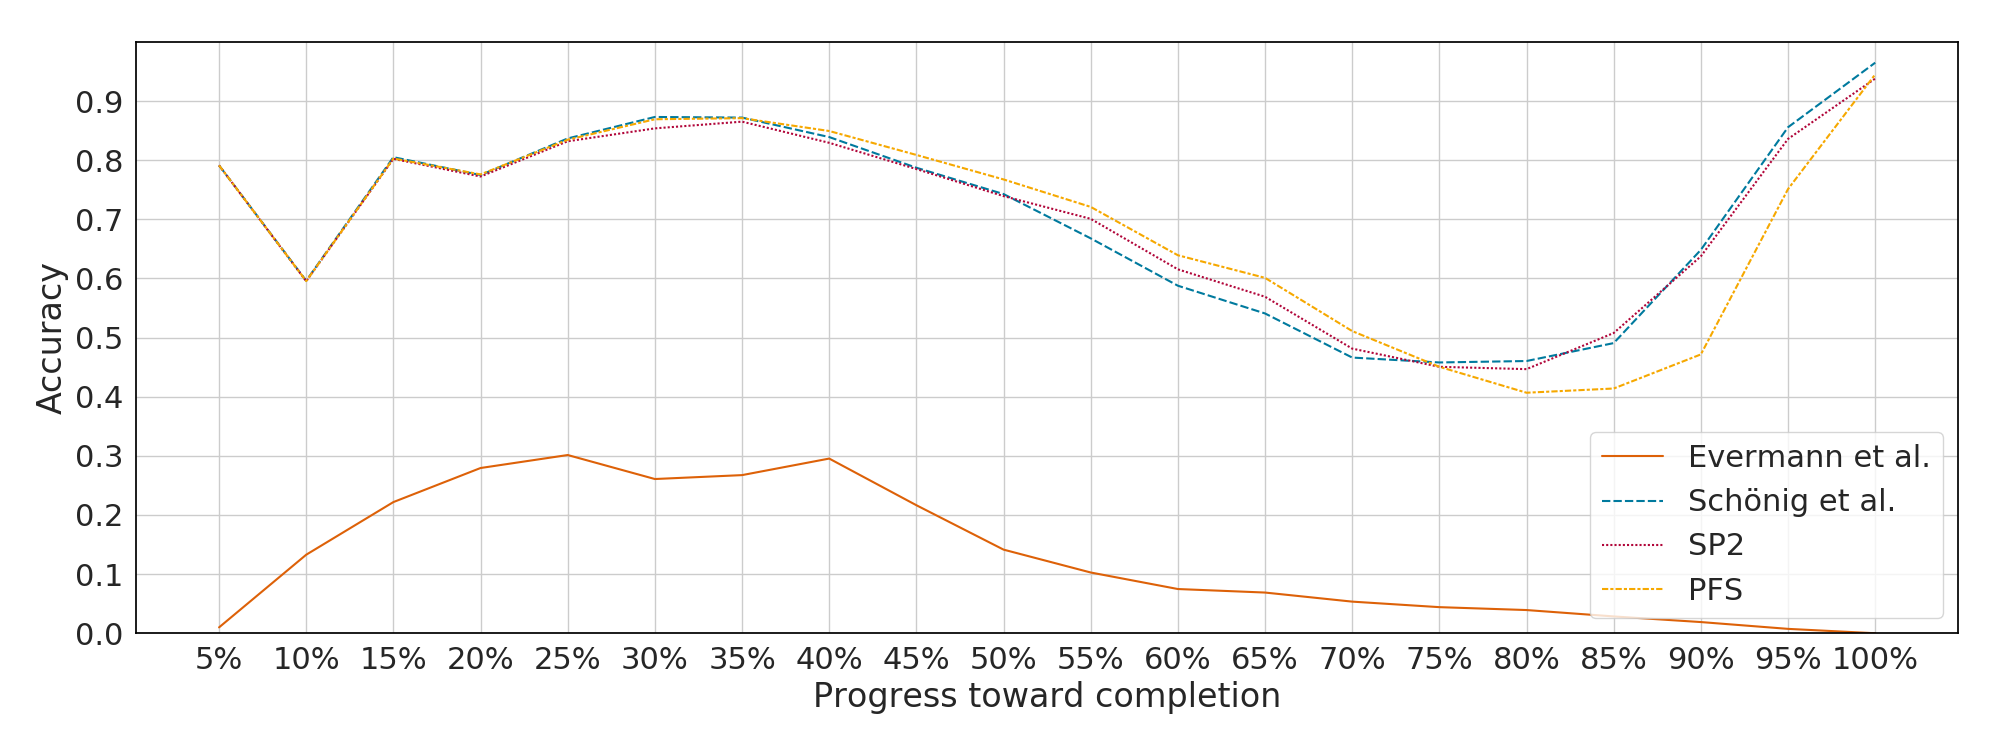
\includegraphics[width=\textwidth]{gfx/bpic2012/padded_stability.png}
    \caption{Stability of the models with the padded batching strategy on BPIC12}
    \label{fig:bpic12-padded-stability}
\end{figure}
\begin{figure}[!htb]
    \centering
    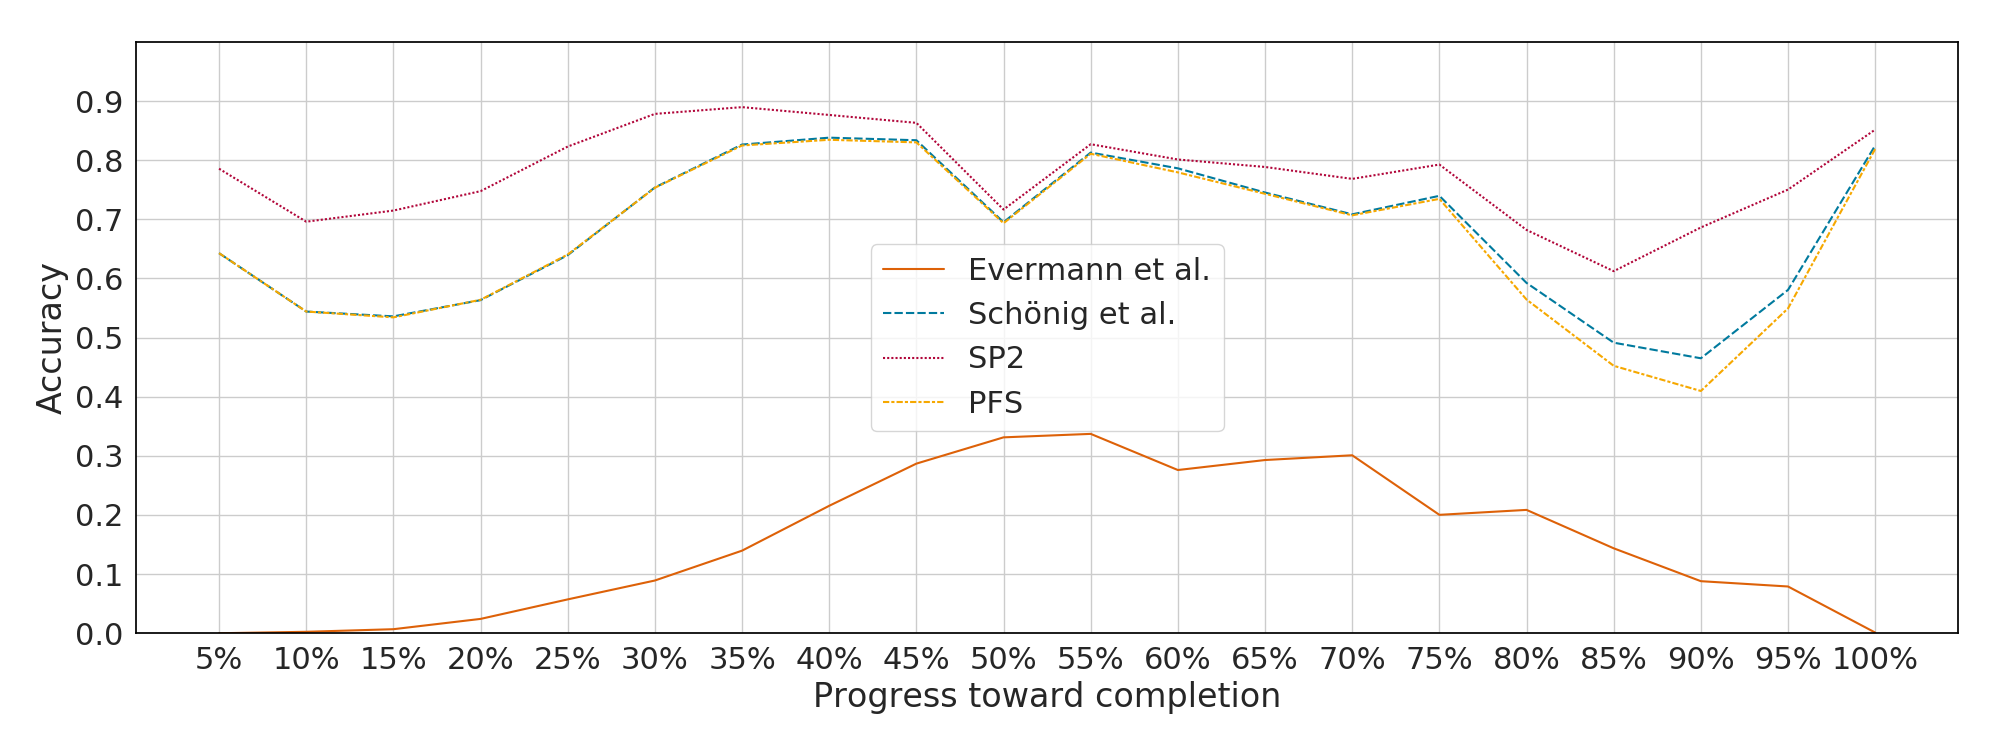
\includegraphics[width=\textwidth]{gfx/bpic2012/windowed_stability.png}
    \caption{Stability of the models with the windowed batching strategy on BPIC12}
    \label{fig:bpic12-windowed-stability}
\end{figure}
\FloatBarrier

\section*{BPIC15-1}
\begin{figure}[!htb]
    \centering
    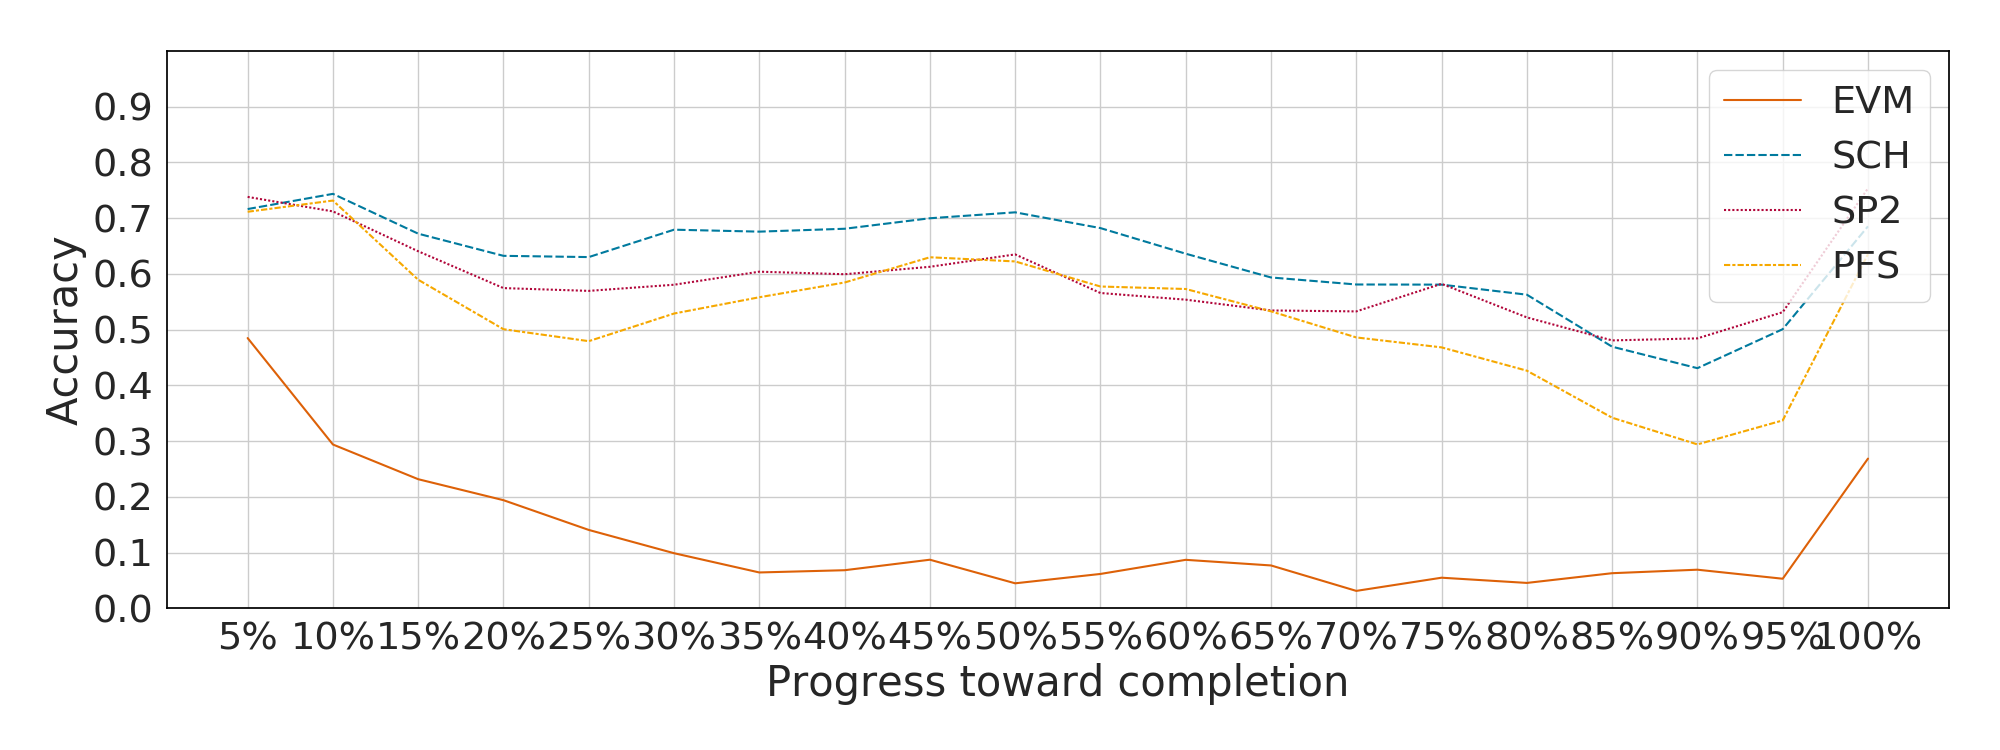
\includegraphics[width=\textwidth]{gfx/bpic2015_1/individual_stability.png}
    \caption{Stability of the models with the individual batching strategy on BPIC15-1}
    \label{fig:bpic15-1-individual-stability}
\end{figure}
\begin{figure}[!htb]
    \centering
    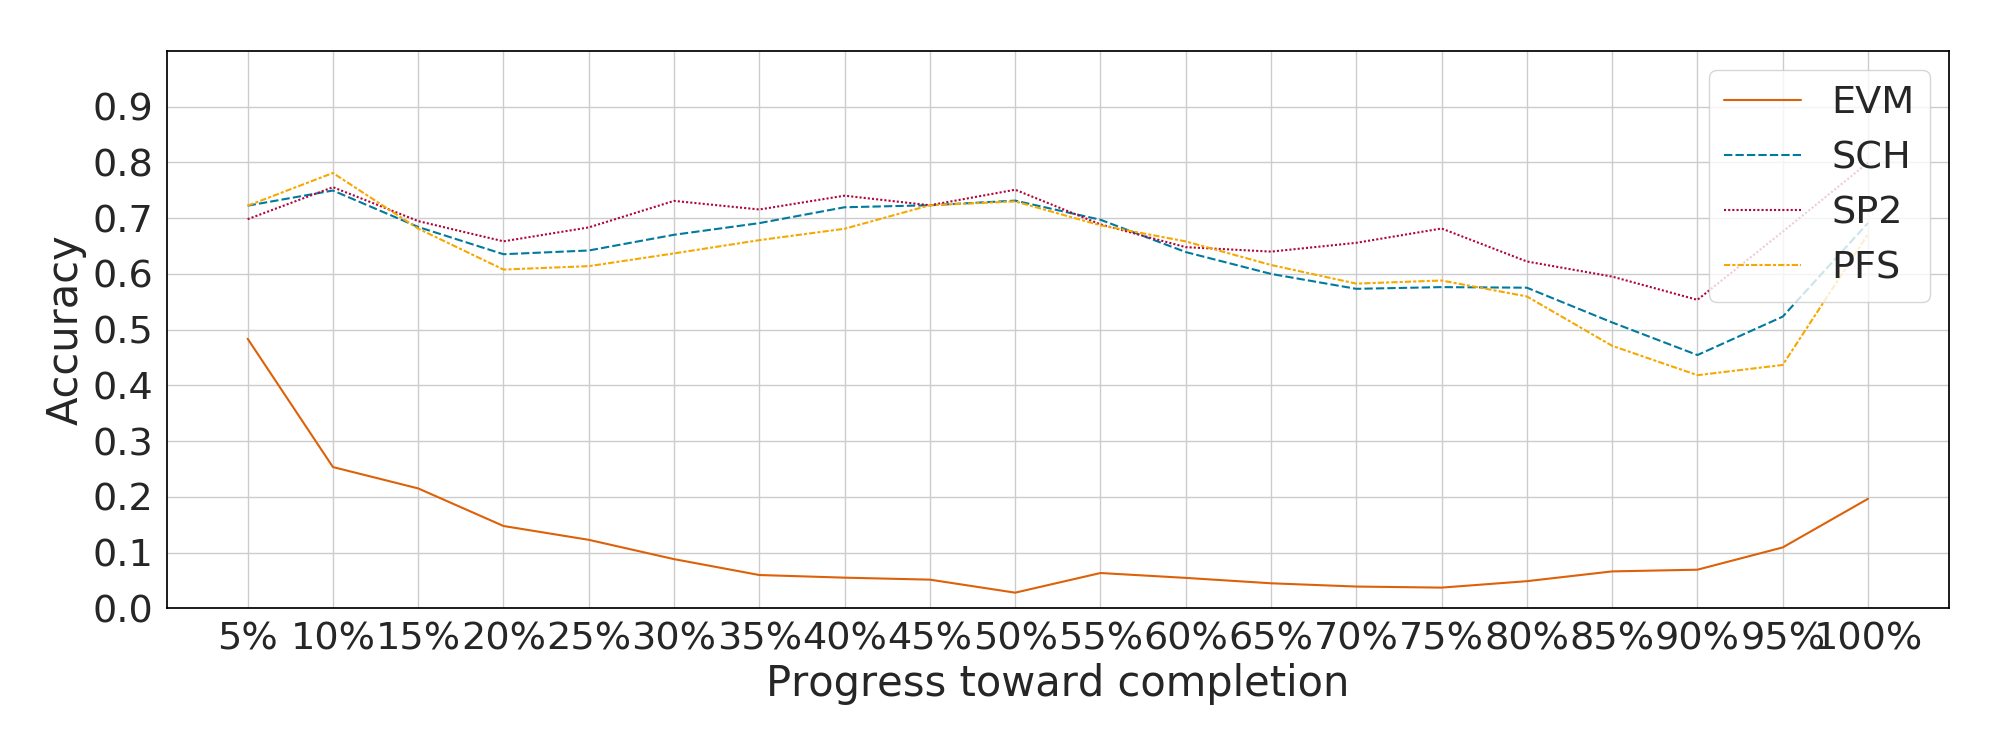
\includegraphics[width=\textwidth]{gfx/bpic2015_1/grouped_stability.png}
    \caption{Stability of the models with the grouped batching strategy on BPIC15-1}
    \label{fig:bpic15-1-grouped-stability}
\end{figure}
\begin{figure}[!htb]
    \centering
    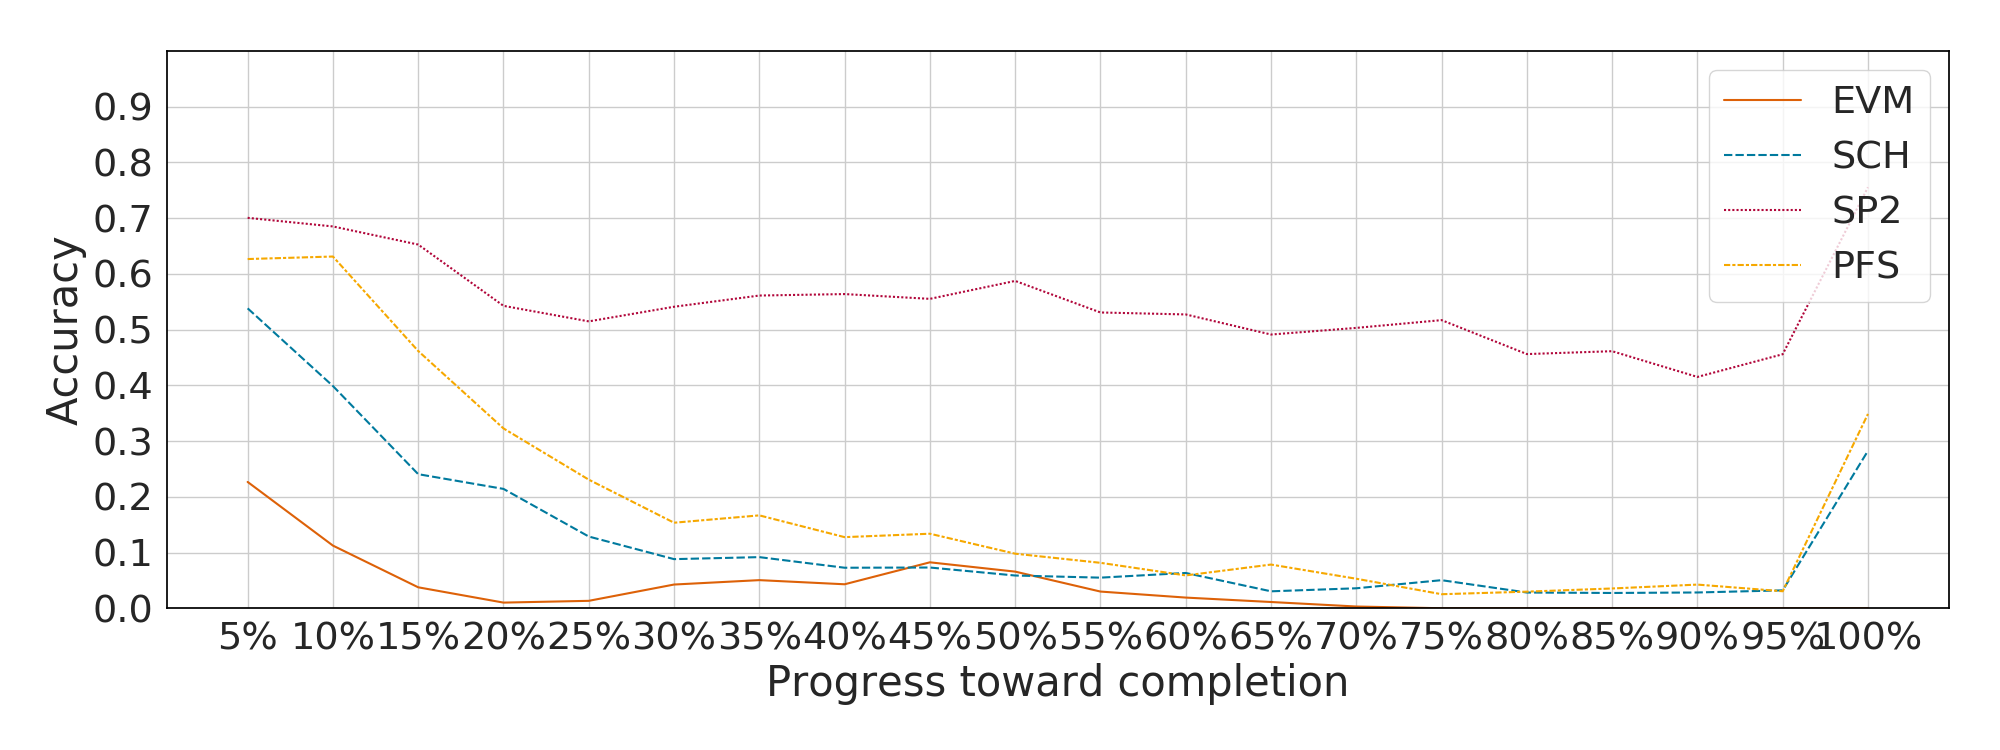
\includegraphics[width=\textwidth]{gfx/bpic2015_1/padded_stability.png}
    \caption{Stability of the models with the padded batching strategy on BPIC15-1}
    \label{fig:bpic15-1-padded-stability}
\end{figure}
\begin{figure}[!htb]
    \centering
    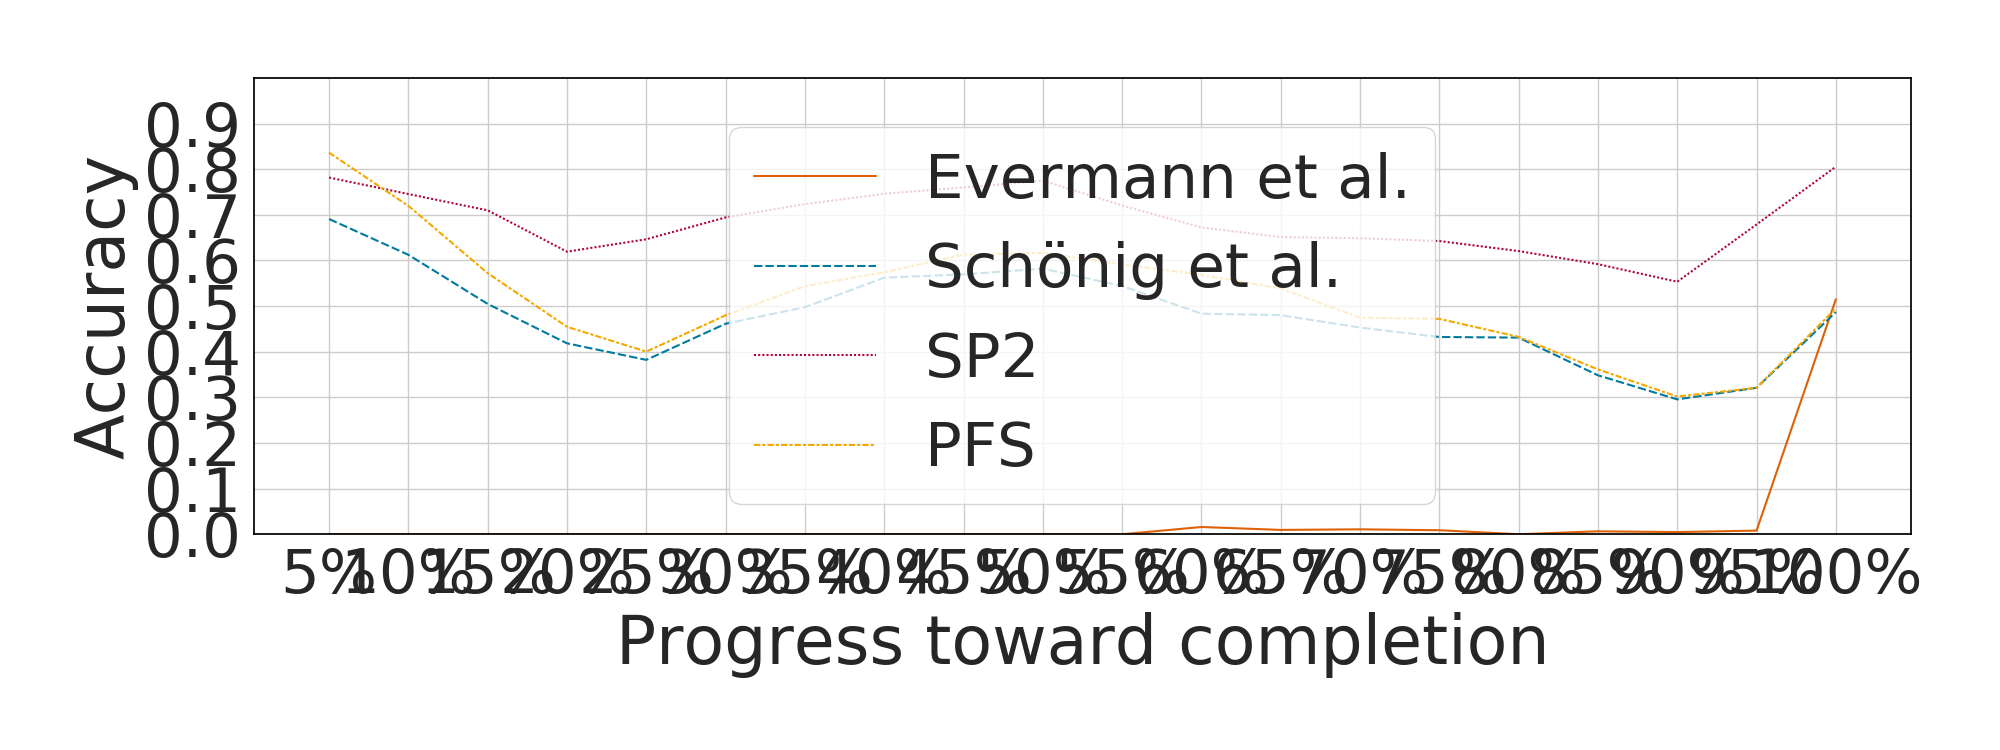
\includegraphics[width=\textwidth]{gfx/bpic2015_1/windowed_stability.png}
    \caption{Stability of the models with the windowed batching strategy on BPIC15-1}
    \label{fig:bpic15-1-windowed-stability}
\end{figure}

\FloatBarrier
\section*{BPIC15-2}
\begin{figure}[!htb]
    \centering
    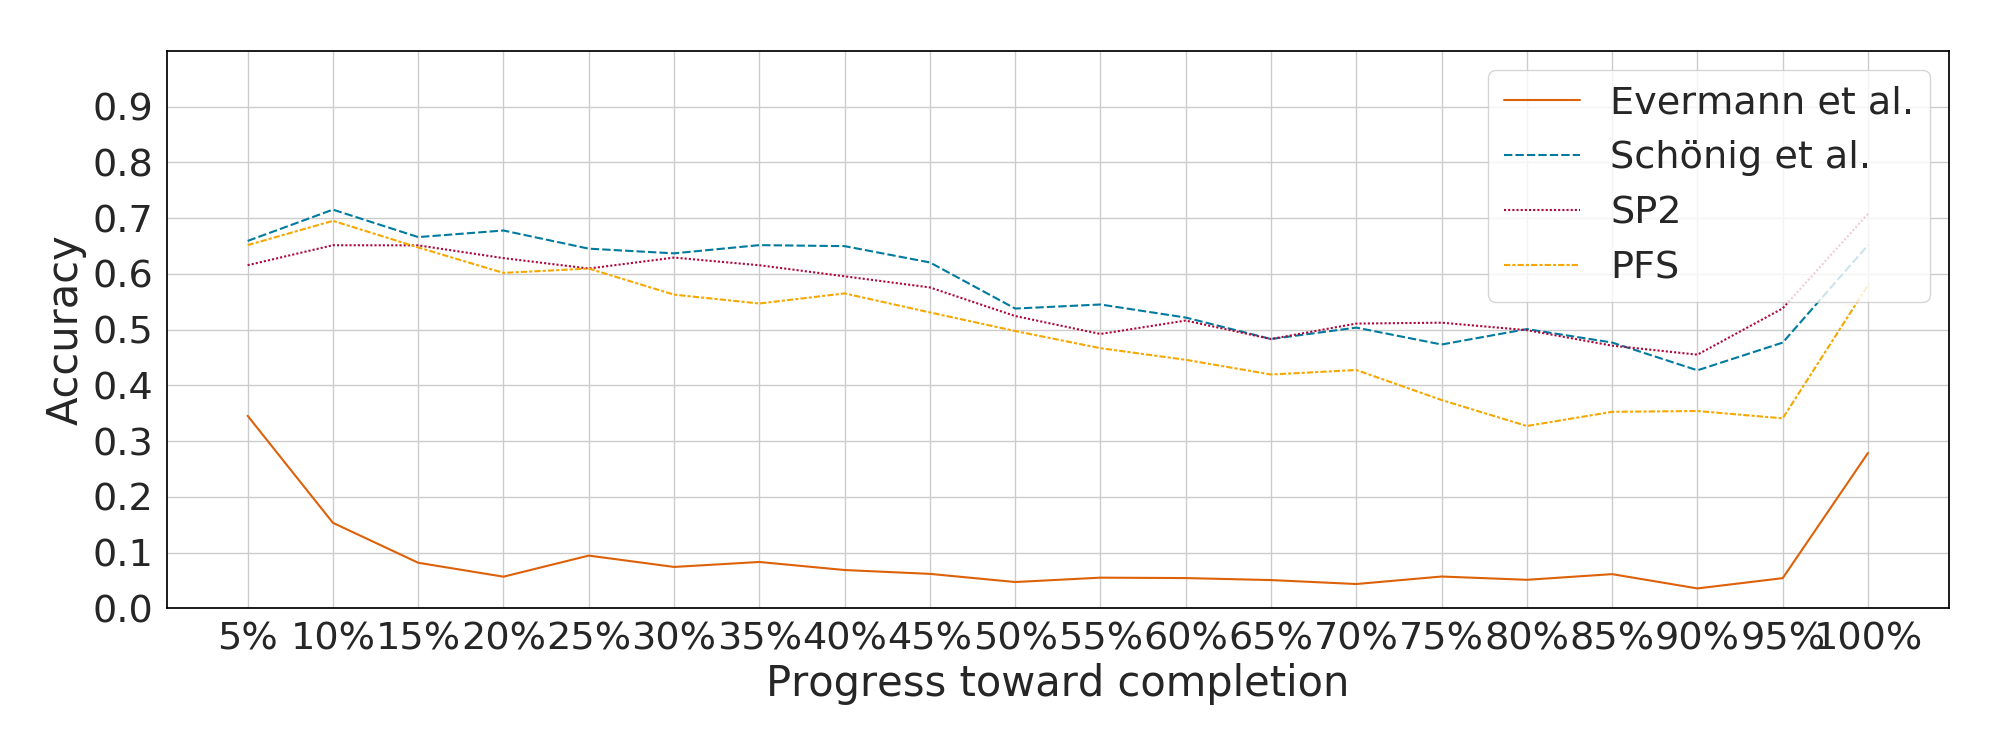
\includegraphics[width=\textwidth]{gfx/bpic2015_2/individual_stability.png}
    \caption{Stability of the models with the individual batching strategy on BPIC15-2}
    \label{fig:bpic15-2-individual-stability}
\end{figure}
\begin{figure}[!htb]
    \centering
    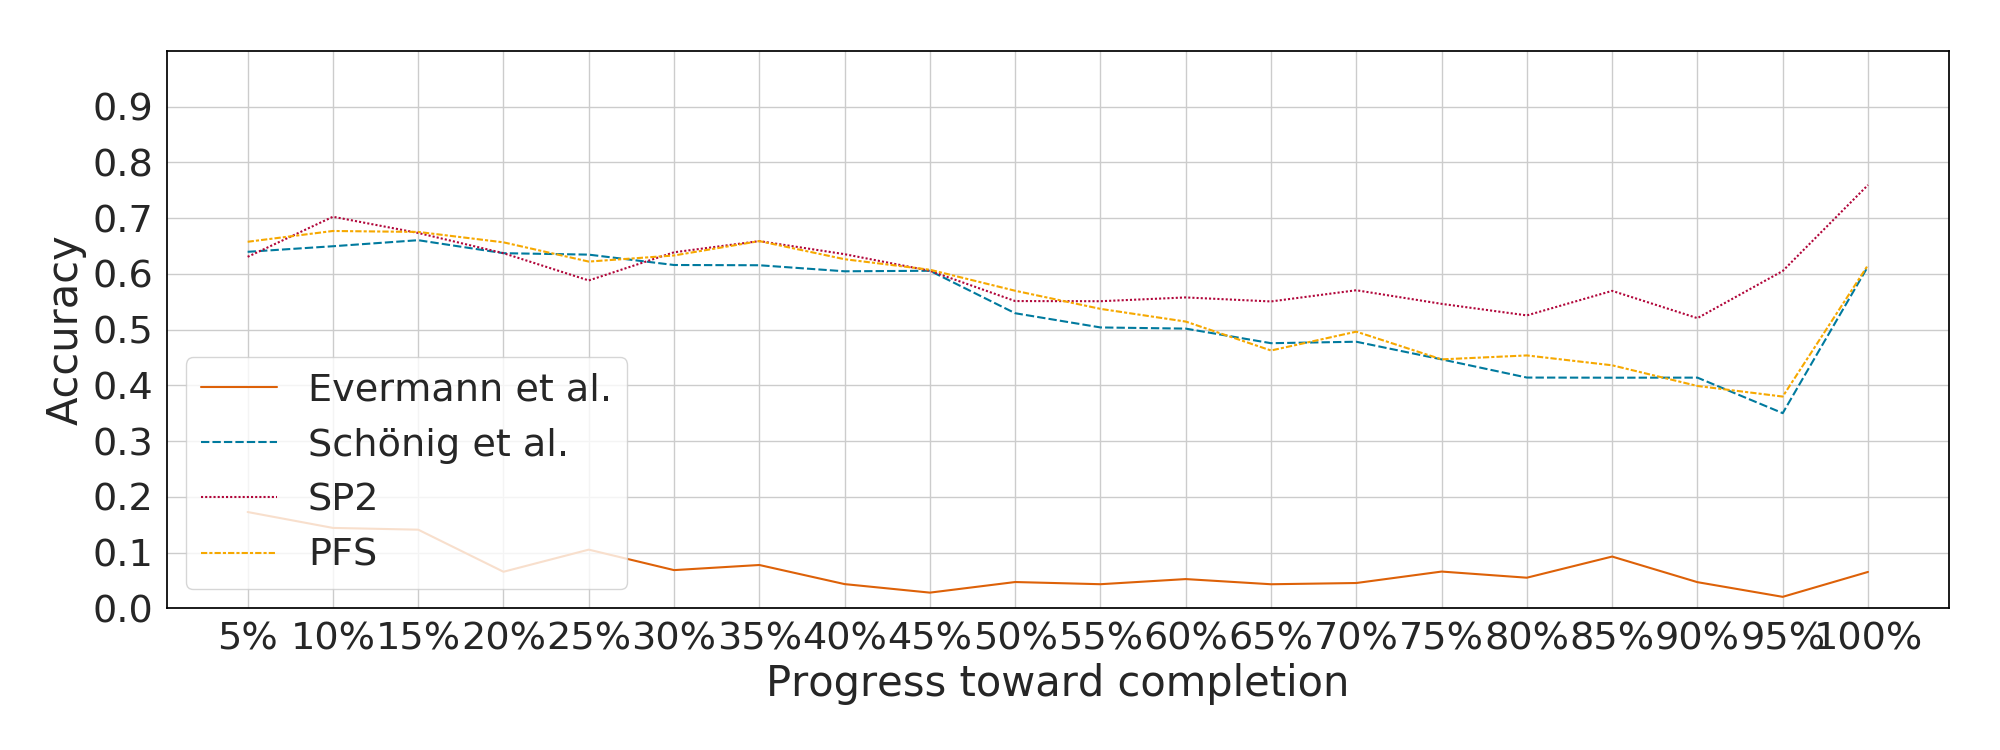
\includegraphics[width=\textwidth]{gfx/bpic2015_2/grouped_stability.png}
    \caption{Stability of the models with the grouped batching strategy on BPIC15-2}
    \label{fig:bpic15-2-grouped-stability}
\end{figure}
\begin{figure}[!htb]
    \centering
    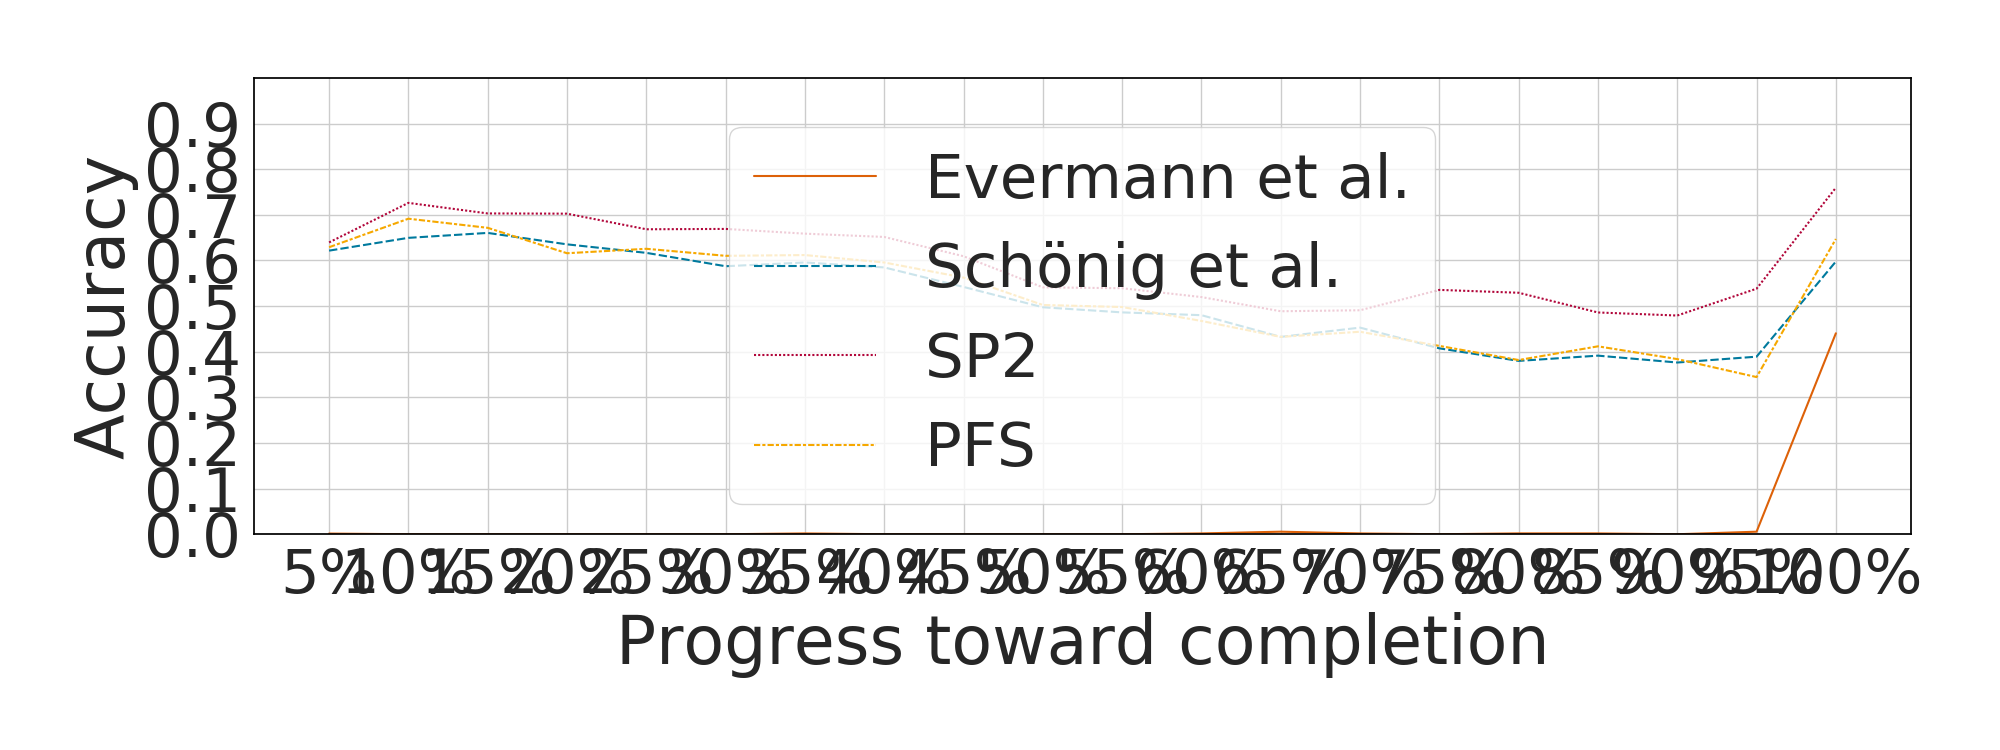
\includegraphics[width=\textwidth]{gfx/bpic2015_2/padded_stability.png}
    \caption{Stability of the models with the padded batching strategy on BPIC15-2}
    \label{fig:bpic15-2-padded-stability}
\end{figure}
\begin{figure}[!htb]
    \centering
    \includegraphics[width=\textwidth]{gfx/bpic2015_2/windowed_stability.png}
    \caption{Stability of the models with the windowed batching strategy on BPIC15-2}
    \label{fig:bpic15-2-windowed-stability}
\end{figure}

\FloatBarrier
\section*{BPIC15-3}
\begin{figure}[!htb]
    \centering
    \includegraphics[width=\textwidth]{gfx/bpic2015_3/individual_stability.png}
    \caption{Stability of the models with the Individual batching strategy on BPIC15-3}
    \label{fig:bpic15-3-individual-stability}
\end{figure}
\begin{figure}[!htb]
    \centering
    \includegraphics[width=\textwidth]{gfx/bpic2015_3/grouped_stability.png}
    \caption{Stability of the models with the grouped batching strategy on BPIC15-3}
    \label{fig:bpic15-3-grouped-stability}
\end{figure}
\begin{figure}[!htb]
    \centering
    \includegraphics[width=\textwidth]{gfx/bpic2015_3/padded_stability.png}
    \caption{Stability of the models with the padded batching strategy on BPIC15-3}
    \label{fig:bpic15-3-padded-stability}
\end{figure}
\begin{figure}[!htb]
    \centering
    \includegraphics[width=\textwidth]{gfx/bpic2015_3/windowed_stability.png}
    \caption{Stability of the models with the windowed batching strategy on BPIC15-3}
    \label{fig:bpic15-3-windowed-stability}
\end{figure}

\FloatBarrier
\section*{BPIC15-4}
\begin{figure}[!htb]
    \centering
    \includegraphics[width=\textwidth]{gfx/bpic2015_4/individual_stability.png}
    \caption{Stability of the models with the individual batching strategy on BPIC15-4}
    \label{fig:bpic15-4-individual-stability}
\end{figure}
\begin{figure}[!htb]
    \centering
    \includegraphics[width=\textwidth]{gfx/bpic2015_4/grouped_stability.png}
    \caption{Stability of the models with the grouped batching strategy on BPIC15-4}
    \label{fig:bpic15-4-grouped-stability}
\end{figure}
\begin{figure}[!htb]
    \centering
    \includegraphics[width=\textwidth]{gfx/bpic2015_4/padded_stability.png}
    \caption{Stability of the models with the padded batching strategy on BPIC15-4}
    \label{fig:bpic15-4-padded-stability}
\end{figure}
\begin{figure}[!htb]
    \centering
    \includegraphics[width=\textwidth]{gfx/bpic2015_4/windowed_stability.png}
    \caption{Stability of the models with the windowed batching strategy on BPIC15-4}
    \label{fig:bpic15-4-windowed-stability}
\end{figure}

\FloatBarrier
\section*{BPIC15-5}
\begin{figure}[!htb]
    \centering
    \includegraphics[width=\textwidth]{gfx/bpic2015_5/individual_stability.png}
    \caption{Stability of the models with the individual batching strategy on BPIC15-5}
    \label{fig:bpic15-5-individual-stability}
\end{figure}
\begin{figure}[!htb]
    \centering
    \includegraphics[width=\textwidth]{gfx/bpic2015_5/grouped_stability.png}
    \caption{Stability of the models with the grouped batching strategy on BPIC15-5}
    \label{fig:bpic15-5-grouped-stability}
\end{figure}
\begin{figure}[!htb]
    \centering
    \includegraphics[width=\textwidth]{gfx/bpic2015_5/padded_stability.png}
    \caption{Stability of the models with the padded batching strategy on BPIC15-5}
    \label{fig:bpic15-5-padded-stability}
\end{figure}
\begin{figure}[!htb]
    \centering
    \includegraphics[width=\textwidth]{gfx/bpic2015_5/windowed_stability.png}
    \caption{Stability of the models with the windowed batching strategy on BPIC15-5}
    \label{fig:bpic15-5-windowed-stability}
\end{figure}

\renewcommand{\thefigure}{C.\arabic{figure}}
\chapter{Accuracy and loss training curves}
\label{appendix:loss-curves}

\section*{BPIC11}
\begin{figure}[!htb]
    \centering
    \includegraphics[width=\textwidth]{gfx/bpic2011/individual_loss_acc_curve.png}
    \caption{Caption}
\end{figure}
\begin{figure}[!htb]
    \centering
    \includegraphics[width=\textwidth]{gfx/bpic2011/grouped_loss_acc_curve.png}
    \caption{Caption}
\end{figure}
\begin{figure}[!htb]
    \centering
    \includegraphics[width=\textwidth]{gfx/bpic2011/padded_loss_acc_curve.png}
    \caption{Caption}
\end{figure}
\begin{figure}[!htb]
    \centering
    \includegraphics[width=\textwidth]{gfx/bpic2011/windowed_loss_acc_curve.png}
    \caption{Caption}
\end{figure}
\FloatBarrier

\section*{BPIC12}
\begin{figure}[!htb]
    \centering
    \includegraphics[width=\textwidth]{gfx/bpic2012/individual_loss_acc_curve.png}
    \caption{Caption}
\end{figure}
\begin{figure}[!htb]
    \centering
    \includegraphics[width=\textwidth]{gfx/bpic2012/grouped_loss_acc_curve.png}
    \caption{Caption}
\end{figure}
\begin{figure}[!htb]
    \centering
    \includegraphics[width=\textwidth]{gfx/bpic2012/padded_loss_acc_curve.png}
    \caption{Caption}
\end{figure}
\begin{figure}[!htb]
    \centering
    \includegraphics[width=\textwidth]{gfx/bpic2012/windowed_loss_acc_curve.png}
    \caption{Caption}
\end{figure}
\FloatBarrier

\section*{BPIC15-1}
\begin{figure}[!htb]
    \centering
    \includegraphics[width=\textwidth]{gfx/bpic2015_1/individual_loss_acc_curve.png}
    \caption{Caption}
\end{figure}
\begin{figure}[!htb]
    \centering
    \includegraphics[width=\textwidth]{gfx/bpic2015_1/grouped_loss_acc_curve.png}
    \caption{Caption}
\end{figure}
\begin{figure}[!htb]
    \centering
    \includegraphics[width=\textwidth]{gfx/bpic2015_1/padded_loss_acc_curve.png}
    \caption{Caption}
\end{figure}
\begin{figure}[!htb]
    \centering
    \includegraphics[width=\textwidth]{gfx/bpic2015_1/windowed_loss_acc_curve.png}
    \caption{Caption}
\end{figure}
\FloatBarrier

\section*{BPIC15-2}
\begin{figure}[!htb]
    \centering
    \includegraphics[width=\textwidth]{gfx/bpic2015_2/individual_loss_acc_curve.png}
    \caption{Caption}
\end{figure}
\begin{figure}[!htb]
    \centering
    \includegraphics[width=\textwidth]{gfx/bpic2015_2/grouped_loss_acc_curve.png}
    \caption{Caption}
\end{figure}
\begin{figure}[!htb]
    \centering
    \includegraphics[width=\textwidth]{gfx/bpic2015_2/padded_loss_acc_curve.png}
    \caption{Caption}
\end{figure}
\begin{figure}[!htb]
    \centering
    \includegraphics[width=\textwidth]{gfx/bpic2015_2/windowed_loss_acc_curve.png}
    \caption{Caption}
\end{figure}
\FloatBarrier

\section*{BPIC15-3}
\begin{figure}[!htb]
    \centering
    \includegraphics[width=\textwidth]{gfx/bpic2015_3/individual_loss_acc_curve.png}
    \caption{Caption}
\end{figure}
\begin{figure}[!htb]
    \centering
    \includegraphics[width=\textwidth]{gfx/bpic2015_3/grouped_loss_acc_curve.png}
    \caption{Caption}
\end{figure}
\begin{figure}[!htb]
    \centering
    \includegraphics[width=\textwidth]{gfx/bpic2015_3/padded_loss_acc_curve.png}
    \caption{Caption}
\end{figure}
\begin{figure}[!htb]
    \centering
    \includegraphics[width=\textwidth]{gfx/bpic2015_3/windowed_loss_acc_curve.png}
    \caption{Caption}
\end{figure}
\FloatBarrier

\section*{BPIC15-4}
\begin{figure}[!htb]
    \centering
    \includegraphics[width=\textwidth]{gfx/bpic2015_4/individual_loss_acc_curve.png}
    \caption{Caption}
\end{figure}
\begin{figure}[!htb]
    \centering
    \includegraphics[width=\textwidth]{gfx/bpic2015_4/grouped_loss_acc_curve.png}
    \caption{Caption}
\end{figure}
\begin{figure}[!htb]
    \centering
    \includegraphics[width=\textwidth]{gfx/bpic2015_4/padded_loss_acc_curve.png}
    \caption{Caption}
\end{figure}
\begin{figure}[!htb]
    \centering
    \includegraphics[width=\textwidth]{gfx/bpic2015_4/windowed_loss_acc_curve.png}
    \caption{Caption}
\end{figure}
\FloatBarrier

\section*{BPIC15-5}
\begin{figure}[!htb]
    \centering
    \includegraphics[width=\textwidth]{gfx/bpic2015_5/individual_loss_acc_curve.png}
    \caption{Caption}
\end{figure}
\begin{figure}[!htb]
    \centering
    \includegraphics[width=\textwidth]{gfx/bpic2015_5/grouped_loss_acc_curve.png}
    \caption{Caption}
\end{figure}
\begin{figure}[!htb]
    \centering
    \includegraphics[width=\textwidth]{gfx/bpic2015_5/padded_loss_acc_curve.png}
    \caption{Caption}
\end{figure}
\begin{figure}[!htb]
    \centering
    \includegraphics[width=\textwidth]{gfx/bpic2015_5/windowed_loss_acc_curve.png}
    \caption{Caption}
\end{figure}
\FloatBarrier

\renewcommand{\thefigure}{D.\arabic{figure}}
\chapter{Trace length distributions}
\label{appendix:trace-length-distributions}

%----------------------------------------------------------------------------------------
%	POST-CONTENT THESIS PAGES
%----------------------------------------------------------------------------------------

\cleardoublepage% Bibliography

\label{app:bibliography} % Reference the bibliography elsewhere with \autoref{app:bibliography}

\manualmark % Work-around to have small caps also here in the headline
\markboth{\spacedlowsmallcaps{\bibname}}{\spacedlowsmallcaps{\bibname}} % Work-around to have small caps also
%\phantomsection
\refstepcounter{dummy}

\addtocontents{toc}{\protect\vspace{\beforebibskip}} % Place the bibliography slightly below the rest of the document content in the table of contents
\addcontentsline{toc}{chapter}{\tocEntry{\bibname}}

\printbibliography[nottype=online]
\printbibliography[heading=subbibliography,title={Online Sources},type=online,prefixnumbers={@}] % Bibliography

\cleardoublepage% Declaration

\refstepcounter{dummy}
\pdfbookmark[0]{Declaration}{declaration} % Bookmark name visible in a PDF viewer

\chapter*{Declaration} % Declaration section text

\thispagestyle{empty}

I certify that the material contained in this thesis is my own work and does not contain significant portions of unreferenced or unacknowledged material. I also warrant that the above statement applies to the implementation of the project and all associated documentation.\\\\
Hiermit versichere ich, dass diese Arbeit selbständig verfasst wurde und dass keine anderen Quellen und Hilfsmittel als die angegebenen benutzt wurden. Diese Aussage trifft auch für alle Implementierungen und Dokumentationen im Rahmen dieses Projektes zu.
\bigskip

\noindent\textit{\myLocation, \myTime}

\smallskip

\begin{flushright}
\begin{tabular}{m{5cm}}
\\ \hline
\centering\myName \\
\end{tabular}
\end{flushright}
 % Declaration

\cleardoublepage% Colophon (a brief description of publication or production notes relevant to the edition)

\pagestyle{empty}

\hfill

\vfill

\pdfbookmark[0]{Colophon}{colophon}

\section*{Colophon}

This document was typeset using the typographical look-and-feel \texttt{classicthesis} developed by Andr\'e Miede. The style was inspired by Robert Bringhurst's seminal book on typography ``\emph{The Elements of Typographic Style}''. \texttt{classicthesis} is available for both \LaTeX\ and \mLyX: 

\begin{center}
\url{https://bitbucket.org/amiede/classicthesis/}
\end{center}

\noindent Happy users of \texttt{classicthesis} usually send a real postcard to the author, a collection of postcards received so far is featured here: 

\begin{center}
\url{http://postcards.miede.de/}
\end{center}
 
\bigskip

\noindent\finalVersionString % Colophon

%----------------------------------------------------------------------------------------

\end{document}
